\documentclass[lettersize,journal]{IEEEtran}
\usepackage{amsmath,amsfonts}
\usepackage{algorithmic}
\usepackage{algorithm}
\usepackage{array}
\usepackage[caption=false,font=normalsize,labelfont=sf,textfont=sf]{subfig}
\usepackage{textcomp}
\usepackage{stfloats}
\usepackage{url}
\usepackage{verbatim}
\usepackage{graphicx}
\usepackage{cite}
\usepackage{tabularx}
\usepackage{booktabs}
\hyphenation{op-tical net-works semi-conduc-tor IEEE-Xplore}
% updated with editorial comments 8/9/2021

\begin{document}

\title{Optical Integrated Sensing and Communication: A Systematic Review of Fiber, Free-Space, VLC/LiFi, and Photonic-THz Platforms}

\author{Fatih D\"onmez, Ahmet Altuncu, and Mustafa Namdar%
\thanks{Fatih D\"onmez and Ahmet Altuncu are with the Department of Electrical and Electronics Engineering, Afyon Kocatepe University, Afyonkarahisar, Turkey (e-mail: fatih.donmez@usr.aku.edu.tr; aaltuncu@aku.edu.tr). Fatih D\"onmez ORCID: 0000-0003-0553-4418. Corresponding author: Fatih D\"onmez.}%
\thanks{Mustafa Namdar is with the Department of Electrical and Electronics Engineering, Faculty of Engineering, Dumlupinar University, C-B.213, 43100, Kutahya, Turkey (e-mail: mustafa.namdar@dpu.edu.tr).}}

\markboth{Draft Manuscript}%
{D\"onmez \MakeLowercase{\textit{et al.}}: Optical Integrated Sensing and Communication Review}

\maketitle

\begin{abstract}
Optical Integrated Sensing and Communication (O-ISAC) is emerging as a promising 6G direction because optical carriers can jointly support ultra-high-rate links and high-resolution sensing across both guided and wireless settings. However, the literature remains fragmented across fiber, free-space optics, VLC/LiFi, and photonic-THz systems, and prior survey-style works do not provide a PRISMA-grounded, cross-modality, metric-governed synthesis.

This systematic review synthesizes 220 peer-reviewed O-ISAC studies and builds a unified framework for comparing heterogeneous optical platforms without collapsing physically distinct metrics. We first establish the physical-layer foundations of O-ISAC and then develop a cross-modality taxonomy spanning medium class, integration style, detection regime, and task specialization. We further introduce a reporting contract that separates bandwidth-limited resolution, estimator-level accuracy, information-theoretic bounds, and plane-specific signal-quality metrics, enabling governed trade-off analysis through admissible rate-resolution views and conservative capacity-resolution quotient (CRQ) synthesis. Beyond performance reporting, we synthesize enabling technologies such as machine learning, optical RIS, optical phased arrays, and photonics-assisted high-frequency generation; map cross-domain applications and transfer opportunities; and consolidate the field into five challenge domains covering standardization, hardware scalability, channel modeling and evaluation, security and reliability, and deployment convergence.

The resulting manuscript does not treat O-ISAC as a single monolithic architecture. Instead, it offers an evidence-backed roadmap for when cross-paper comparison is defensible, where current deployment evidence concentrates, and which research bottlenecks most strongly shape credible 6G-facing O-ISAC systems.
\end{abstract}

\begin{IEEEkeywords}
Optical integrated sensing and communication, O-ISAC, free-space optics, visible light communication, distributed fiber sensing, photonic-terahertz systems, systematic review.
\end{IEEEkeywords}

\section{Introduction}
\label{introduction}
\subsection{The Convergence of Sensing and Communication: A 6G Imperative}
\IEEEPARstart{T}{he} escalating complexity of the electromagnetic environment has intensified demand for wireless systems that can communicate and sense jointly. ISAC is therefore now treated as a core 6G enabler and is recognized by both the ITU-R IMT-2030 framework and 3GPP as part of the future service landscape \cite{O_ISAC_070,O_ISAC_162}. Emerging applications such as robot navigation, augmented reality, autonomous driving, and human--machine interaction increasingly require high-rate communication and high-accuracy environmental awareness in the same workflow \cite{O_ISAC_016,O_ISAC_351}. Yet even with strong progress in RF-based ISAC, the migration toward mmWave and THz does not remove three persistent constraints:

\begin{enumerate}
    \item \textbf{Spectrum Congestion}: RF communication and sensing remain constrained by scarce spectrum, growing interference pressure, and increasing competition from data-hungry mobile services \cite{O_ISAC_068,O_ISAC_161}.
    \item \textbf{Limited Resolution and Bandwidth}: mmWave RF-ISAC remains fundamentally constrained in bandwidth and sensing resolution, often falling short of millimeter-precision targets while incurring high power and capability limits \cite{O_ISAC_021,O_ISAC_203}.
    \item \textbf{Hardware Constraints}: Purely electrical mmWave/THz generation struggles to deliver the bandwidth and reconfigurability expected for 6G without substantial hardware complexity and cost \cite{O_ISAC_070,O_ISAC_286}.
\end{enumerate}

\textbf{Optical Integrated Sensing and Communication (O-ISAC)} addresses these limits by unifying perception, transmission, and processing on optical carriers \cite{O_ISAC_021}. As summarized in Fig.~\ref{fig:fig1}, optical carriers open access to the 28.3--845 THz design space and naturally branch into fiber, free-space, VLC/LiFi, and optical--THz-bridging settings. Across the 220-study corpus considered here, representative prototypes already report \textbf{120 Gbps wireless throughput with 2.5 mm sensing resolution} in photonic-THz integration \cite{O_ISAC_105} and \textbf{241.85 Tb/s aggregate transmission with concurrent sensing} in seven-core fiber systems \cite{O_ISAC_046}. These results motivate the central question of this review: which physical properties of the optical domain enable such gains, and how can they be synthesized under a defensible cross-modality framework?

\begin{figure*}[!t]
    \centering
    
\includegraphics[width=\linewidth]{figures/fig1.png}
    \caption{Evolution of O-ISAC: (A) RF-ISAC faces spectrum and hardware limits, (B) optical carriers expose broad photonic resources ($\approx$28.3--845 THz), and (C) this review organizes O-ISAC into fiber, free-space/photo-THz, and VLC/LiFi branches with distinct signal and impairment models.}
    \label{fig:fig1}
\end{figure*}

These exemplars define the rate--resolution frontier considered throughout the manuscript. We next examine the physical foundations that make the optical domain a natural substrate for high-performance ISAC.

Table~\ref{tab:axis_comparison} previews the axis-based comparison of related review- and survey-style works discussed in Section I-D.

\begin{table*}[!t]
\caption{Comparison of this review with representative related review- and survey-style works across scope, methodology, and analytical coverage axes}
\label{tab:axis_comparison}
\centering
\footnotesize
\setlength{\tabcolsep}{3.2pt}
\renewcommand{\arraystretch}{1.15}

\begin{tabularx}{\textwidth}{@{}%
>{\centering\arraybackslash}p{1.35cm}
>{\centering\arraybackslash}p{0.68cm}
>{\centering\arraybackslash}p{0.62cm}
>{\centering\arraybackslash}X
>{\centering\arraybackslash}p{0.82cm}
>{\centering\arraybackslash}p{0.90cm}
>{\centering\arraybackslash}p{0.72cm}
>{\centering\arraybackslash}p{0.82cm}
>{\centering\arraybackslash}p{0.88cm}
>{\centering\arraybackslash}p{0.90cm}
>{\centering\arraybackslash}p{0.95cm}
@{}}
\toprule
\multicolumn{6}{c}{\textbf{Positioning and Review Type}} &
\multicolumn{5}{c}{\textbf{Analytical Coverage}} \\
\cmidrule(lr){1-6}\cmidrule(lr){7-11}
\textbf{Ref.} &
\textbf{Year} &
\textbf{Tier} &
\textbf{\shortstack{Modality Scope\\(Fiber / FSO / VLC / P-THz)}} &
\textbf{\shortstack{Int.\\Depth}} &
\textbf{Method} &
\textbf{Tax.} &
\textbf{Metrics} &
\textbf{Bench.} &
\textbf{Transfer} &
\textbf{Enablers} \\
\midrule

\cite{O_ISAC_161} & 2025 & 2 & $\circ/\circ/\circ/\circ$ & $\bullet$  & Rev.   & $\oslash$ & --        & --        & --        & --        \\
\cite{O_ISAC_068} & 2023 & 2 & $\circ/\circ/\bullet/\circ$ & $\bullet$  & Narr.  & --        & --        & --        & --        & --        \\
\cite{O_ISAC_327} & 2024 & 2 & $\circ/\circ/\bullet/\circ$ & $\oslash$  & Surv.  & $\oslash$ & --        & --        & --        & --        \\
\cite{O_ISAC_006} & 2024 & 2 & $\bullet/\circ/\circ/\circ$ & $\oslash$  & Rev.   & --        & $\oslash$ & --        & --        & --        \\
\cite{O_ISAC_368} & 2023 & 2 & $\bullet/\circ/\circ/\circ$ & $\oslash$  & Rev.   & --        & --        & --        & --        & --        \\
\cite{O_ISAC_021} & 2023 & 2 & $\circ/\bullet/\circ/\circ$ & $\bullet$  & Tut.   & $\oslash$ & $\oslash$ & --        & --        & $\oslash$ \\
\cite{O_ISAC_070} & 2025 & 2 & $\circ/\circ/\circ/\bullet$ & $\bullet$  & Narr.  & $\oslash$ & --        & --        & --        & --        \\
\cite{O_ISAC_163} & 2025 & 2 & $\circ/\circ/\circ/\circ$ & $\bullet$  & Surv.  & $\oslash$ & --        & --        & $\oslash$ & $\bullet$ \\
\cite{O_ISAC_303} & 2024 & 1 & $\circ/\circ/\bullet/\circ$ & $\bullet$  & Rev.   & $\oslash$ & $\oslash$ & --        & --        & --        \\

\midrule
\textbf{This Review} &
\textbf{2026} &
\textbf{--} &
\textbf{$\bullet/\bullet/\bullet/\bullet$} &
$\bullet$ &
\textbf{PRISMA} &
$\bullet$ &
$\bullet$ &
$\bullet$ &
$\bullet$ &
$\bullet$ \\
\bottomrule
\end{tabularx}

\vspace{2pt}
\footnotesize
\emph{Notation:} $\bullet$ = strong/explicit; $\oslash$ = partial/within-modality; -- = absent; 
$\circ$ = out-of-scope. Modality scope is reported in the order \textbf{F / FSO / VLC / THz}, 
with THz restricted here to photonic-THz or optical--THz bridging O-ISAC.\\
\emph{Scoring rule:} For analytical axes, $\{--,\oslash,\bullet\}\mapsto\{0,\tfrac{1}{2},1\}$.
The symbol $\circ$ is used only for modality-scope exclusion and is not scored.
\end{table*}

\subsection{The Optical Opportunity: A Vast and Untapped Frontier}
The optical domain expands the design space far beyond congested sub-300 GHz RF bands, nominally spanning approximately \textbf{28.3 THz to 845 THz}, though practical systems cluster in atmospheric transmission windows and fiber telecom bands \cite{O_ISAC_021}. In this review, Photo-THz O-ISAC denotes photonics-enabled architectures in which optical carriers support generation/LO/distribution while wireless propagation occurs in the sub-THz/THz band. The rest of this subsection isolates the physical advantages that make that spectrum attractive for next-generation ISAC.
\subsubsection{Quantitative Comparison: RF-ISAC vs. O-ISAC}

Table~\ref{tab:performance_comparison} provides a compact RF-ISAC versus O-ISAC comparison using representative ranges from the reviewed corpus \cite{O_ISAC_021}.

\begin{table*}[!t]
\caption{RF-ISAC vs. O-ISAC Performance Comparison \protect\cite{O_ISAC_021}}
\label{tab:performance_comparison}
\centering
\footnotesize
\setlength{\tabcolsep}{3.2pt}
\renewcommand{\arraystretch}{1.15}

\begin{tabularx}{\textwidth}{@{}%
>{\raggedright\arraybackslash}p{2.35cm}
>{\raggedright\arraybackslash}X
>{\raggedright\arraybackslash}X
>{\raggedright\arraybackslash}X
@{}}
\toprule
\textbf{Characteristic} &
\textbf{RF-ISAC (Sub-6 GHz / mmWave)} &
\textbf{Wireless O-ISAC (FSO / VLC / Photo-THz)} &
\textbf{Wired O-ISAC (Fiber Sensing)} \\
\midrule

\textbf{Carrier Frequency} &
2.4--100 GHz &
0.1--10 THz (Photo-THz) + 28.3--845 THz (FSO/VLC) &
193 THz (C-band / L-band) \\

\textbf{Physics Model} &
Diffuse multipath (rich) &
LoS-dominated propagation &
Guided mode (low-loss, dispersive) \\

\textbf{Signal Type} &
Complex (I/Q) &
Real (IM/DD) or complex (coherent FSO) &
Complex (coherent phase/polarization) \\

\textbf{Key Impairments} &
Interference, multipath fading &
Ambient light, turbulence, pointing error &
Kerr nonlinearity, PMD, phase noise \\

\textbf{Sensing Task} &
Radar (range/Doppler) &
Localization, gesture, surface profiling &
DAS (vibration), strain, temperature \\

\textbf{Peak Data Rate} &
$\sim$10--20 Gbps &
\textbf{$\sim$100--120 Gbps} \cite{O_ISAC_105} &
\textbf{$>$200 Tbps} (aggregate) \cite{O_ISAC_046} \\

\textbf{Resolution} &
cm-level &
\textbf{mm-level (2.5 mm)} \cite{O_ISAC_105} &
m-level (spatial) / $n\varepsilon$ (strain) \\
\bottomrule
\end{tabularx}

\vspace{2pt}
\footnotesize
\emph{Abbreviations:} RF = radio frequency; FSO = free-space optics; VLC = visible light communication; 
Photo-THz denotes photonic-THz or optical--THz bridging links; DAS = distributed acoustic sensing; 
IM/DD = intensity modulation/direct detection; PMD = polarization mode dispersion.
\end{table*}

\subsubsection{Three Competitive Advantages of O-ISAC}

Following \cite{O_ISAC_021}, we group the optical advantage into three mechanisms: capacity scaling, bandwidth-limited sensing precision, and directional spatial isolation. Fig.~\ref{fig:fig2} summarizes the underlying physics.

\begin{figure*}[!t]
    \centering
    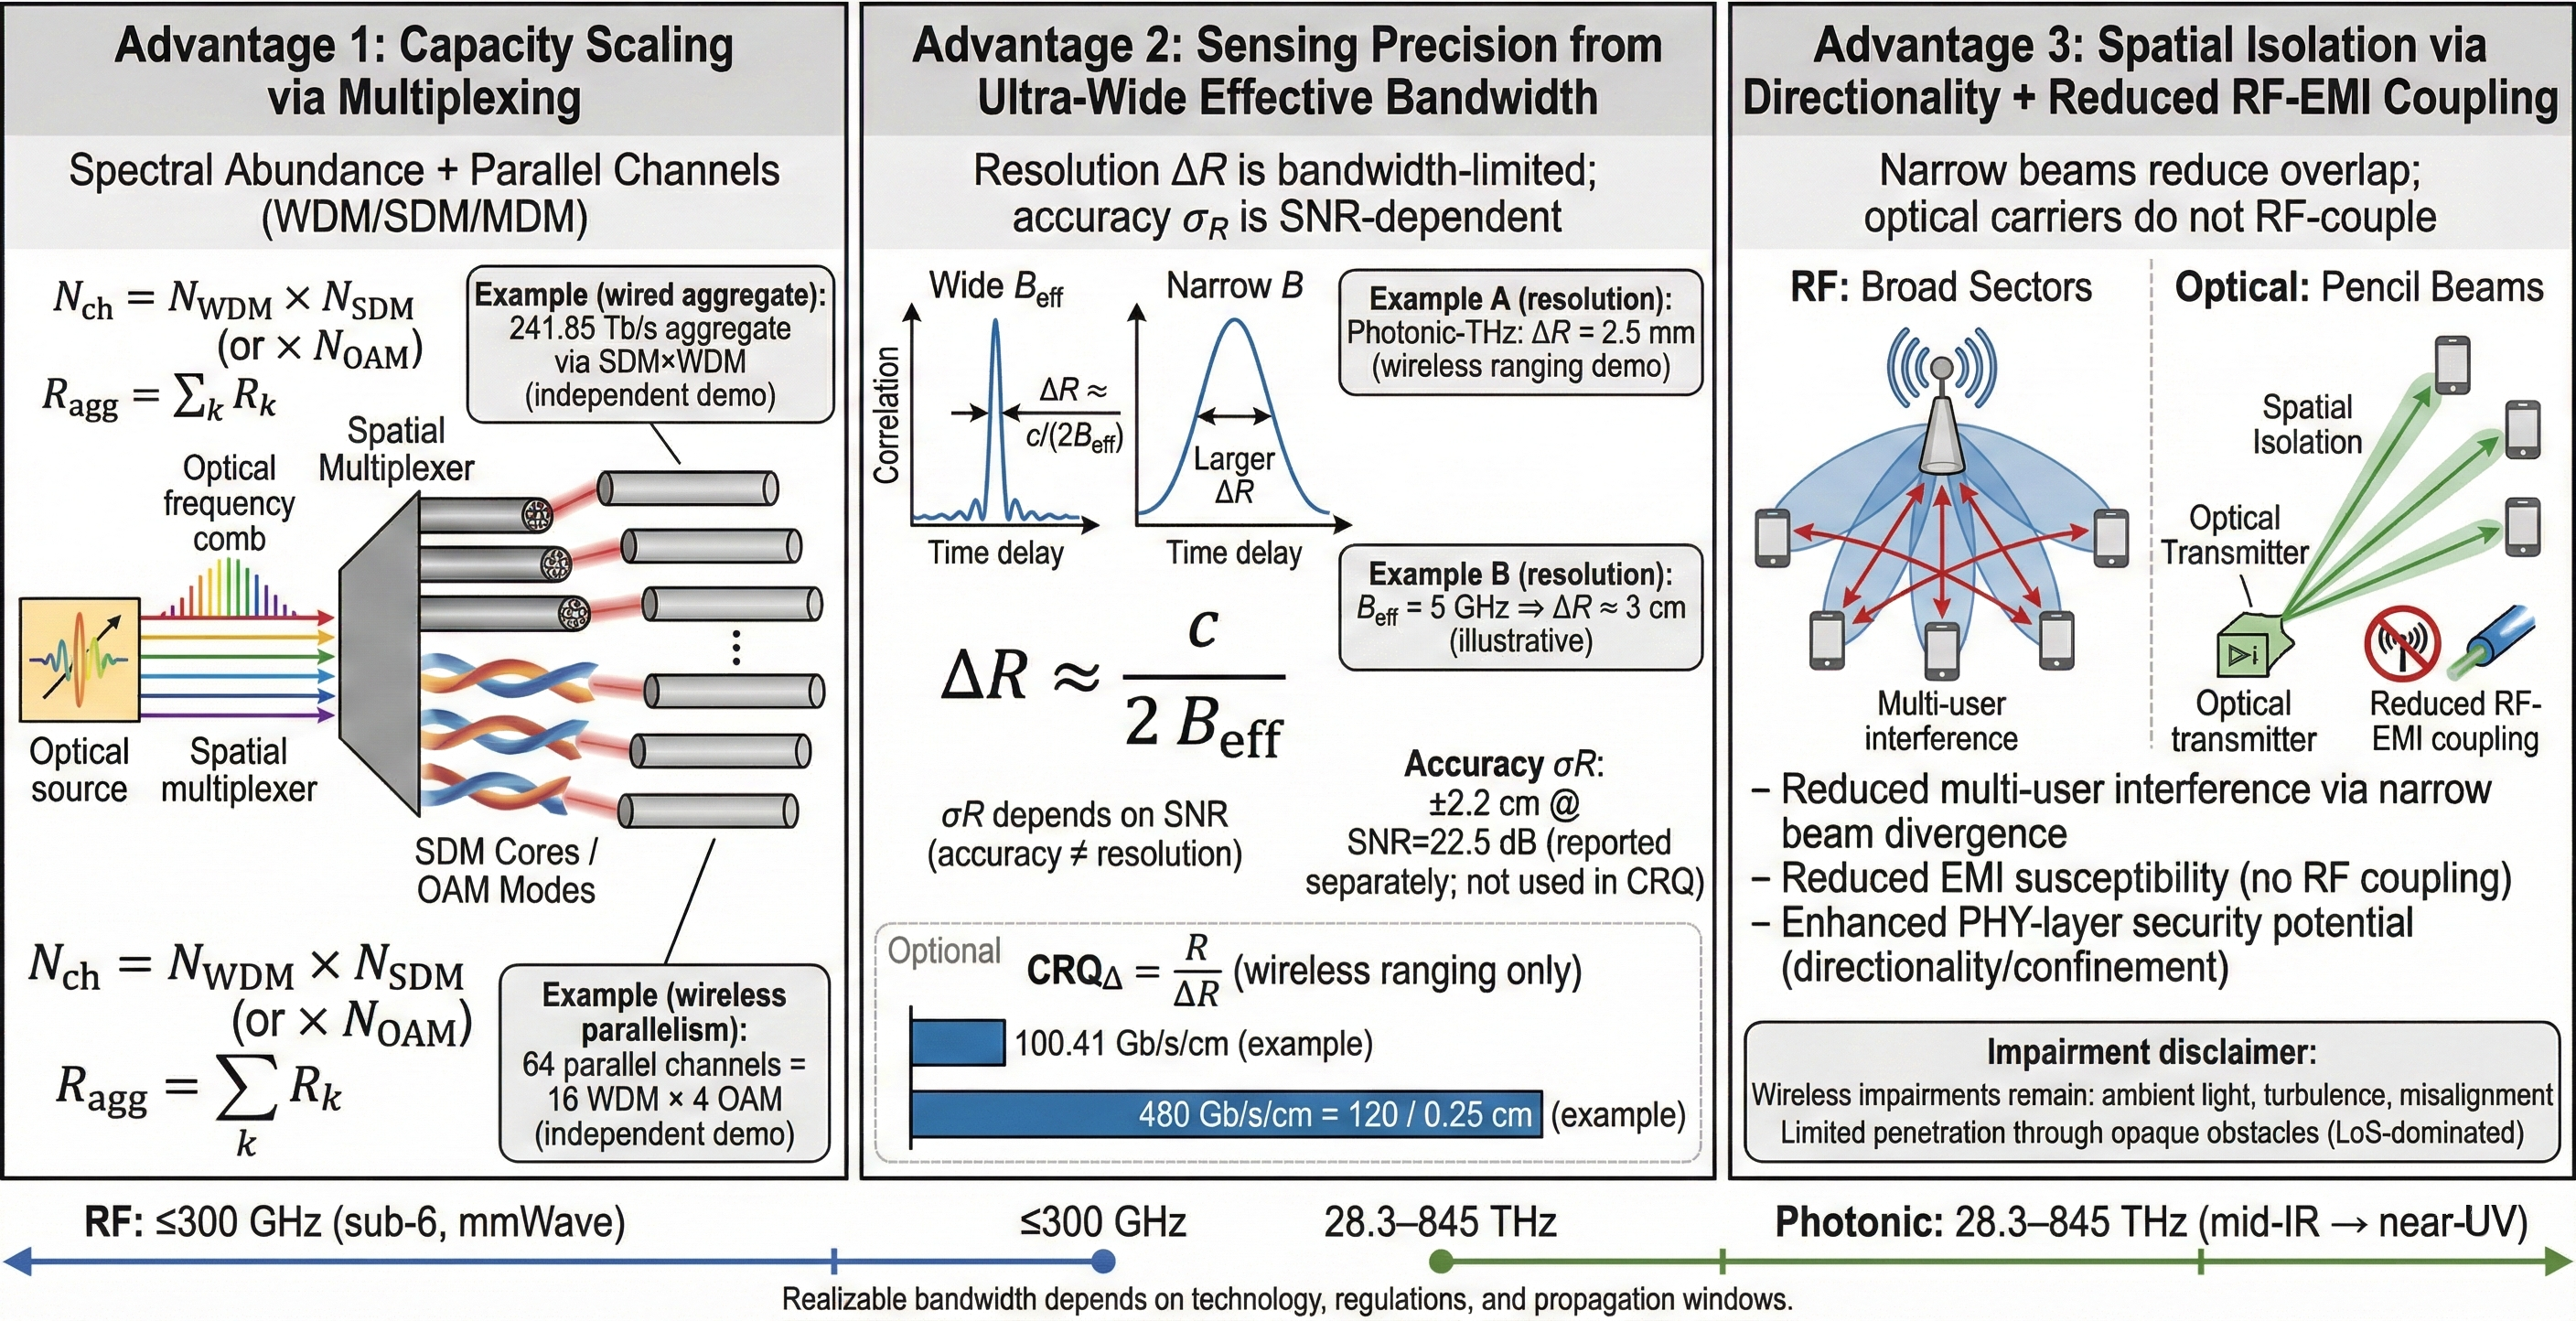
\includegraphics[width=\linewidth]{figures/fig2.png}
    \caption{Physical basis of the three optical advantages: dense multiplexing for capacity scaling, ultra-wide effective bandwidth for fine ranging and high $\text{CRQ}_{\Delta}$, and narrow beams for spatial isolation with lower RF-EMI coupling.}
    \label{fig:fig2}
\end{figure*}

\paragraph{Advantage 1: Capacity Scaling Through Spectral Abundance and Multiplexing}
The optical spectrum supports dense multiplexing well beyond RF-sized blocks. In wireless settings, MDM combined with WDM has realized \textbf{64 parallel channels} (16 wavelengths $\times$ 4 OAM modes) \cite{O_ISAC_021}; in cabled settings, 7-core SDM fiber has reached \textbf{241.85 Tbps} over 38 km \cite{O_ISAC_046}. Together, these results validate optical parallelism beyond single-link RF limits.

\paragraph{Advantage 2: Enhancing Sensing Precision via Ultra-Wide Bandwidth}
Range resolution in two-way sensing is bandwidth-limited as $\Delta r_{\min} = v/(2B_{\text{eff}})$. Optical bandwidths therefore enable wireless ranging regimes that narrowband RF systems struggle to match: photonic-THz demonstrations report \textbf{2.5 mm} resolution alongside 120 Gbps, giving $\text{CRQ}_{\Delta} = 4.8\times10^{13}$ bps/m \cite{O_ISAC_105}. Throughout this review, we keep this bandwidth-limited resolution distinct from SNR-dependent estimation accuracy such as RMSE/$\sigma_r$; fiber DAS contributes through sensitive distributed monitoring rather than fine free-space range resolution \cite{O_ISAC_046}.

\paragraph{Advantage 3: Spatial Isolation and Reduced RF-EMI Coupling}
The high directionality of optical beams provides deployment-dependent spatial isolation and can reduce multi-user interference relative to wide-beam RF sectors in clear line-of-sight settings \cite{O_ISAC_021}. Wireless O-ISAC still faces turbulence and ambient-light sensitivity \cite{O_ISAC_003}, but its weak coupling to conventional RF electromagnetic interference and milliradian-scale beam divergence support dense spatial reuse when propagation conditions are favorable.


\subsection{Unified O-ISAC Taxonomy}

Having established the optical advantages, we next delimit the scope of this review. O-ISAC is not a single monolithic system class; it clusters into modality families shaped by propagation medium, signal model, and dominant impairment. Fig.~\ref{fig:fig3} previews the evidence-based taxonomy from our PRISMA-compliant corpus, centered on 2020--2025 while retaining a small number of earlier protocol-eligible foundational studies: fiber, free-space optical, VLC/LiFi, and photonic-THz, each with distinct operating windows and sensing--communication conventions.


\begin{figure*}[!t]
    \centering
    
\includegraphics[width=\linewidth]{figures/fig3.png}
    \caption{Preview of the four modality families in the 220-study PRISMA corpus: fiber, FSO, VLC/LiFi, and photonic-THz, distinguished by operating window, dominant impairment, and representative sensing--communication tasks.}
    \label{fig:fig3}
\end{figure*}

This shared reference frame is essential for later cross-modality comparison, but it also exposes a deeper issue: terminology, metrics, and evaluation protocols remain inconsistent across communities. That inconsistency motivates the fragmentation challenge discussed next.

\subsection{The Fragmentation Challenge: A Landscape Without Unity}

Despite these physical advantages, the O-ISAC literature remains fragmented. Our systematic analysis of \textbf{220 peer-reviewed studies}, primarily from \textbf{2020--2025}, reveals four recurring fault lines: inconsistent terminology, non-standardized sensing metrics, siloed modality communities, and weak cross-domain technology transfer. Together, they impede reproducibility and defensible cross-study comparison.

\textbf{Terminology Proliferation.} Closely related ideas are labeled differently across communities: RF-oriented work still uses aliases such as RadCom and JRC \cite{O_ISAC_161}, VLC papers alternate between JCS, ISAC, and SCI \cite{O_ISAC_068}, and fiber work diverges into labels such as ISAC-OF, fiber-ISAC, and photonic ISAC \cite{O_ISAC_041,O_ISAC_033}. This aliasing complicates systematic discovery, inflates perceived novelty through re-labeling, and obscures conceptual links across modalities.

\textbf{Metric Non-Isomorphism.} Equally problematic is the absence of a shared sensing-performance language. A first-order example is the recurrent conflation of \textbf{physical resolution limits}, \textbf{estimator-dependent accuracy}, and \textbf{information-/estimation-theoretic bounds}. For ranging, the bandwidth-limited physical resolution is
\begin{equation}
\Delta r_{\min}=\frac{v}{2B_{\text{eff}}}
\end{equation}
where $v=c$ in free space and $v\approx c/n_g$ in guided media. In contrast, RMSE/$\sigma_r$ and localization error remain SNR- and estimator-dependent, while CRB/FIM quantities describe information bounds under an explicit observation model \cite{O_ISAC_013,O_ISAC_050,O_ISAC_056}. The same "resolution" label can therefore refer to different objects across modalities, and signal quality also shifts across reference planes: coherent fiber studies often report OSNR \cite{O_ISAC_028}, whereas VLC studies usually report post-detection electrical SNR \cite{O_ISAC_009}.

\textbf{Sub-Domain Siloing and Limited Cross-Citation.} Fiber DAS/communication co-design, FSO ranging links, VLC positioning/data systems, and photonic-THz ISAC have largely evolved in separate channel, hardware, and evaluation cultures \cite{O_ISAC_033,O_ISAC_050,O_ISAC_082}. As a result, a trade-off frontier in one modality is rarely comparable to another without harmonized assumptions. Recent assessments echo this separation, noting weak integration even within VLC/VLP ecosystems and persistent interoperability barriers across sectors \cite{O_ISAC_039,O_ISAC_161}.

\textbf{Weak Cross-Domain Technology Transfer.} Methods developed in one optical sub-domain are only weakly reused in others. Fiber-oriented waveform/probing structures seldom transfer to free-space or VLC links, and VLC-centric localization or learning pipelines rarely reappear in FSO or photonic-THz settings \cite{O_ISAC_042,O_ISAC_074,O_ISAC_022,O_ISAC_039}. Without shared benchmarks and reporting protocols, it remains difficult to separate what is modality-specific from what is genuinely transferable \cite{O_ISAC_068,O_ISAC_067}.

\textbf{The Missing Unifying Framework.} These issues point to the same gap: O-ISAC still lacks a shared physical-layer taxonomy, a standardized reporting contract, and a cross-modality benchmark culture. At minimum, comparable studies should disclose communication performance, sensing performance separated into $\Delta r_{\min}$, estimator-level error, and CRB/FIM-style bounds, signal quality at an explicit reference plane, and the channel/scenario assumptions that govern comparability. Recent calls for standardized VLC channel models and interoperability-oriented standardization reinforce the urgency of this unification \cite{O_ISAC_327,O_ISAC_068,O_ISAC_082}.

\subsection{Related Surveys and Gap Analysis}

RF-ISAC already has a mature survey landscape, but optical ISAC remains comparatively underserved. Existing review-style work is still modality-centric: VLC surveys emphasize positioning and indoor propagation \cite{O_ISAC_068,O_ISAC_327}, fiber reviews focus on DFOS/DAS integration and co-route monitoring \cite{O_ISAC_006,O_ISAC_041,O_ISAC_090}, and FSO or photonic-THz surveys discuss architectures, waveforms, and high-CRQ demonstrations without bridging the full FSO--fiber--VLC divide \cite{O_ISAC_021,O_ISAC_035,O_ISAC_058,O_ISAC_070}. Within our 220-study corpus, only the VLC-based LiSAC review explicitly treats optical ISAC as its primary topic, and even that work remains single-modality and non-PRISMA \cite{O_ISAC_303}. RIS-for-ISAC surveys provide useful enabling-technology context but remain RF/THz-centric \cite{O_ISAC_163}. Table~\ref{tab:axis_comparison} summarizes this landscape.

\textbf{Gap Synthesis.} Five gaps distinguish the current survey landscape from a unified O-ISAC framework. First, there is still no cross-modality taxonomy spanning fiber, FSO, VLC/LiFi, and photo-THz under a single physical-layer abstraction. Second, PRISMA-aligned systematic methodology is absent from the identified optical survey-style works. Third, metric normalization remains unresolved: the literature does not consistently separate $\Delta r_{\min}$, estimator-dependent accuracy, CRB/FIM-style bounds, and reference-plane-specific signal-quality reporting. Fourth, cross-domain technology transfer remains weak. Fifth, enabling technologies such as optical RIS and optical phased arrays are still treated in fragmented, technology-centric ways rather than under a shared integration framework. These gaps collectively motivate the present review as a PRISMA-compliant, cross-modality synthesis.


These gaps collectively establish the rationale for this review: a PRISMA-compliant systematic review that unifies O-ISAC across all four modalities, establishes a standardized taxonomy and reporting contract, and synthesizes quantitative trade-off frontiers to guide future research.

\subsection{Contributions of This Review}
To close the five gaps identified in Section I-D, we provide evidence-backed contributions grounded in the PRISMA corpus and extraction schema; each item includes a compact Contribution-Gap-Section mapping:


\begin{enumerate}
    \item \textbf{PRISMA evidence base and quality scoring (Gap 2):} We apply the PRISMA 2020 protocol \cite{PRISMA2020} to a unified corpus of 220 studies with bibliographic year metadata available for 219 records (210 in 2020-2025), and we report complete 5-dimension TQAF scores for 208 studies. \textit{Contribution-Gap-Section:} Gap 2 $\rightarrow$ Section III.
    \item \textbf{Cross-modality taxonomy with measured coverage (Gap 1):} We construct a unified taxonomy spanning fiber, FSO, VLC/visible-light, photo-THz, and hybrid O-ISAC; the extracted medium labels include 46 fiber, 19 FSO, 26 VLC/visible-light/UV, 1 photo-THz, and 116 hybrid studies (optical-THz bridging can appear under hybrid depending on the extraction label ontology). \textit{Contribution-Gap-Section:} Gap 1 $\rightarrow$ Section IV.
    \item \textbf{Standardized reporting contract and trade-off synthesis (Gap 3):} We normalize reporting using $\Delta r_{\min}$, $\sigma_r$, and $\text{CRQ}_{\Delta}$ and quantify coverage: 217 studies report data-rate metrics, 213 report a resolution-type metric ($\Delta r_{\min}$ in ranging or $\Delta z$/spatial granularity in fiber), 208 report $\sigma_r$, and 171 report CRB/CRLB values; 213 studies report both rate and a resolution-type metric, enabling $\text{CRQ}_{\Delta}$ comparisons where $\Delta r_{\min}$ is available (N\_rate\_and\_resType = 213; N\_rate\_and\_Drmin = 160). \textit{Contribution-Gap-Section:} Gap 3 $\rightarrow$ Section V.
    \item \textbf{Enabler-centric synthesis across optical platforms (Gap 5):} We quantify enabling-technology prevalence to ground Section VI, including machine learning (53 studies), optical RIS (ORIS, 8 studies), and optical phased arrays (OPA, 7 studies), and relate these tags to the integration pathways discussed in the enabler section. \textit{Contribution-Gap-Section:} Gap 5 $\rightarrow$ Section VI.
    \item \textbf{Cross-domain transfer map tied to applications (Gap 4):} We build a modality-application transfer map in Section VII; 15 application domains appear in $\ge$2 modality classes (8 domains in $\ge$3), with high-frequency domains including industrial manufacturing (65), vehicular (60), indoor positioning (56), and 6G networking (46). \textit{Contribution-Gap-Section:} Gap 4 $\rightarrow$ Section VII.
\end{enumerate}

\subsection{Organization of This Paper}

The remainder of this review is organized as follows. Section II establishes the physical-layer fundamentals, Section III details the PRISMA/TQAF methodology, Section IV introduces the unified taxonomy, Section V synthesizes rate-resolution trade-offs, Section VI reviews enabling technologies, Section VII maps applications and transfer patterns, Section VIII consolidates challenge domains and the research roadmap, and Section IX concludes.


\subsection{Notation and Acronyms}

For the reader's convenience, the mathematical notation conventions and the most frequently used acronyms in this paper are defined in Tables~\ref{tab:math_notation} and \ref{tab:acronyms}, respectively.
\begin{table}[!t]
\caption{Mathematical Notation Conventions}
\label{tab:math_notation}
\centering
\footnotesize
\begin{tabularx}{\columnwidth}{@{}>{\raggedright\arraybackslash}p{0.38\columnwidth} >{\raggedright\arraybackslash}X@{}}
\toprule
\textbf{Symbol} & \textbf{Definition} \\
\midrule
$\lambda$ & Optical wavelength (nm) \\
$B_{\mathrm{eff}}$ & Effective signal bandwidth (Hz) \\
$R$ & Data rate (bit/s) \\
$d$ & Target distance or range (m) \\
$\Delta r_{\min}$ & Bandwidth-limited two-way range resolution (m) \\
$\sigma_r = \sqrt{\mathbb{E}[(\hat r - r)^2]}$ & Range estimation error or RMSE (m) \\
$\mathrm{SNR}$ & Signal-to-noise ratio \\
$\mathrm{BER}$ & Bit error rate \\
$\alpha$ & Power allocation factor for communication--sensing trade-off \\
\bottomrule
\end{tabularx}
\end{table}

\begin{table}[!t]
\caption{List of Frequently Used Acronyms}
\label{tab:acronyms}
\centering
\footnotesize
\begin{tabularx}{\columnwidth}{@{}>{\raggedright\arraybackslash}p{2.6cm}>{\raggedright\arraybackslash}X@{}}
\toprule
\textbf{Acronym} & \textbf{Definition} \\
\midrule
\textbf{ISAC} & Integrated Sensing and Communication \\
\textbf{O-ISAC} & Optical Integrated Sensing and Communication \\
\textbf{ISAC-OF} & Integrated Sensing and Communication in Optical Fiber \\
\textbf{DFS} & Distributed Fiber Sensing \\
\textbf{DAS} & Distributed Acoustic Sensing \\
\textbf{VLC} & Visible Light Communication \\
\textbf{FSO} & Free-Space Optical \\
\textbf{OWC} & Optical Wireless Communication \\
\textbf{LFM} & Linear Frequency Modulation \\
\textbf{OFDM} & Orthogonal Frequency Division Multiplexing \\
\textbf{DCO-OFDM} & DC-biased Optical OFDM \\
\textbf{OCDM} & Orthogonal Chirp Division Multiplexing \\
\textbf{IM/DD} & Intensity Modulation / Direct Detection \\
\textbf{ORIS} & Optical Reconfigurable Intelligent Surface \\
\textbf{OPA} & Optical Phased Array \\
\textbf{PIC} & Photonic Integrated Circuit \\
\textbf{CCR} & Corner Cube Reflector \\
\textbf{RO-ISAC} & Retroreflective O-ISAC \\
\textbf{$\phi$-OTDR} & Phase-Sensitive Optical Time-Domain Reflectometry \\
\textbf{SMF} & Single-Mode Fiber \\
\textbf{FMF} & Few-Mode Fiber \\
\textbf{MCF} & Multi-Core Fiber \\
\textbf{WDM} & Wavelength Division Multiplexing \\
\textbf{DSCM} & Digital Subcarrier Multiplexing \\
\textbf{THz} & Terahertz \\
\textbf{MIMO} & Multiple-Input Multiple-Output \\
\textbf{PRISMA} & Preferred Reporting Items for Systematic Reviews and Meta-Analyses \\
\textbf{TQAF} & Technical Quality Assessment Form \\
\textbf{RMSE} & Root Mean Square Error \\
\textbf{CRB} & Cram\'er--Rao Bound \\
\bottomrule
\end{tabularx}
\end{table}


\section{TECHNICAL FUNDAMENTALS OF O-ISAC}
\subsection{Unified O-ISAC System Model and Integration Paradigms}
\subsubsection{Canonical Joint Waveform/Resource Model}
Design rationale: We define a joint design variable set that spans waveform parameters (bandwidth, chirp rate, pilot structure, coding), optical front-end parameters (source, modulation, detection), and sensing-task parameters (range/angle/velocity versus fiber spatial granularity). This compact variable set supports cross-modality comparisons without erasing the physical constraints that distinguish coherent and IM/DD architectures.


\textbf{Generic baseband observation (complex coherent model):}
\begin{equation}
\mathbf{y}(t)=\mathbf{H}(t;\boldsymbol{\theta})\mathbf{s}(t)+\mathbf{w}(t)
\end{equation}
where \(\mathbf{y}(t)\) is the received complex baseband observation, \(\mathbf{s}(t)\) is the transmitted complex baseband waveform, \(\mathbf{H}(t;\boldsymbol{\theta})\) is a parametric operator embedding sensing parameters \(\boldsymbol{\theta}\) (e.g., delay, Doppler, angle), and \(\mathbf{w}(t)\) is receiver noise.

\textbf{IM/DD observation (real, nonnegative intensity constraint):}
\begin{equation}
y(t)=\mathcal{R}\,\big(x(t)\ast h(t)\big)+n(t),\qquad x(t)\ge 0
\end{equation}
where \(y(t)\) is the electrical observation after direct detection, \(x(t)\) is the transmitted optical intensity waveform, \(h(t)\) is the intensity channel impulse response, \(\mathcal{R}\) is photodetector responsivity, and \(n(t)\) is additive electrical noise. Here \(x(t)\) denotes the modulated optical intensity (post square-law abstraction), not the optical field amplitude; the nonnegativity constraint follows.

\textbf{Measurement-plane contract.} We map each reported metric \(m\) to a measurement plane via

\begin{equation}
\label{eq:measurement_plane_contract}
\begin{aligned}
\pi(m)\in\{&\text{OPTICAL\_PLANE},\;\text{ELECTRICAL\_PLANE},\\
&\text{AMBIGUOUS}\}
\end{aligned}
\end{equation}


where OPTICAL\_PLANE refers to pre-detection optical field/power (\(E(t)\), \(P(t)=|E(t)|^2\ge 0\)) and ELECTRICAL\_PLANE refers to post-detection electrical baseband observations. OSNR and electrical SNR must be reported on their native planes, and OSNR-to-SNR conversion is prohibited unless a source provides an explicit receiver model (Metric Governance). Generic ``SNR'' without an optical/electrical cue remains AMBIGUOUS and is not used to justify plane separation (Metric Governance). For ranging tasks, the delay-to-range relation \(\tau=2r/v\) underpins \(\Delta r_{\min}=v/(2B_{\text{eff}})\), whereas fiber DAS reports spatial granularity via \(\Delta z\) (gauge/segment length) rather than \(\Delta r_{\min}\) (Metric Governance).

Evidence alignment: Representative studies report BER against OSNR (explicitly optical signal-to-noise ratio) for coherent optical links \cite{O_ISAC_132,O_ISAC_076}.
Representative studies separately report electrical SNR after photodetection for BER/RMSE evaluation \cite{O_ISAC_061,O_ISAC_100,O_ISAC_023}. Consistent with the governance contract, we keep these as different measurement planes and do not infer one from the other without an explicit receiver/noise model.

\subsubsection{Integration Paradigms (Communication-centric / Sensing-centric / Joint Design)}
Design rationale: For cross-modality synthesis, we classify integration by mechanism (shared waveform, shared hardware, shared time/frequency resources, shared processing) rather than by medium. This mechanism-first lens keeps fiber/FSO/VLC/photonic-THz cases comparable while preserving their physical constraints.


\textbf{Communication-centric:} Communication performance is primary; sensing operates under communication-driven resource limits. A minimal exemplar is maximize \(R\) subject to \(J_{\text{sense}}(\boldsymbol{\theta})\le \varepsilon\).

\textbf{Sensing-centric:} Sensing fidelity is primary; communication is constrained to satisfy a service floor. A minimal exemplar is minimize \(J_{\text{sense}}(\boldsymbol{\theta})\) subject to \(R\ge R_0\) (and/or BER \(\le \beta\)).

\textbf{Joint design:} Communication and sensing are co-optimized as explicit multi-objective trade-offs. A minimal exemplar is minimize \([J_{\text{sense}}(\boldsymbol{\theta}),\; -R]\) (Pareto) or minimize \(\alpha J_{\text{sense}}(\boldsymbol{\theta})-(1-\alpha)R\), where \(R\) is throughput and \(J_{\text{sense}}\) is a sensing loss (e.g., estimation MSE or a ranging-error proxy).

These three paradigms denote operating intent (not mutually exclusive hardware classes); one architecture may move between them by changing constraints or operating point.

Paradigm-to-mechanism bridge:
\begin{itemize}
    \item Communication-centric $\rightarrow$ shared processing / shared resources $\rightarrow$ sensing piggybacks on communication signaling.
    \item Sensing-centric $\rightarrow$ shared waveform / shared hardware $\rightarrow$ communication is embedded under sensing-driven constraints.
    \item Joint design $\rightarrow$ shared waveform + shared processing $\rightarrow$ explicit co-optimization couples both objectives.
\end{itemize}

We define an integration depth variable
\begin{equation}
d_{\text{int}}\in\{0,\;1/2,\;1\}
\end{equation}
where \(d_{\text{int}}=0\) corresponds to coexistence, \(d_{\text{int}}=1/2\) to partial sharing/cooperation, and \(d_{\text{int}}=1\) to full co-design. This internal axis is used later to align taxonomy and trade-off synthesis without rewriting modality-specific models.

Evidence alignment: A.2 defines a review-internal synthesis scaffold for later sections; it does not claim prevalence or superiority of any paradigm in this subsection, so no paper-specific performance claim is asserted here.

\textbf{Fig.~\ref{fig:fig_ii_1}} consolidates this system abstraction into a single review-facing view. It preserves a common source-modulator-waveform-channel-observation-output chain, separates coherent and IM/DD observation paths, and keeps integration paradigms as an interpretive side axis rather than as modality labels.


\begin{figure*}[!t]
    \centering
    
\includegraphics[width=\linewidth]{figures/fig_ii_1.png}
    \caption{Unified O-ISAC system abstraction across modalities. The figure summarizes a common source-modulator-waveform-channel-observation-output chain while retaining modality-conditioned channels, coherent versus IM/DD observations, and communication-centric to joint-design integration depths.}
   \label{fig:fig_ii_1}
\end{figure*}

\subsection{Propagation and Channel Models Across Modalities}
This subsection defines a modality-aware channel layer for O-ISAC. The aim is not to rank modalities, but to expose dominant propagation impairments under a common operator view. The measurement-plane contract from Section II-A remains binding: channel modeling does not justify OSNR-to-SNR conversion, and optical/electrical plane separation is preserved.

\subsubsection{Fiber Channel (Guided Medium)}
Design rationale: Fiber links are naturally represented by a linear dispersive baseband model in most communication analyses, with nonlinear wave dynamics added when launch power and distance require it.

A baseline model is
\begin{equation}
\mathbf{y}(t)=\mathbf{G}_{\mathrm{disp}}(t)\ast \mathbf{s}(t)+\mathbf{w}(t)
\label{eq:fiber_linear_model}
\end{equation}
where $\mathbf{G}_{\mathrm{disp}}(t)$ captures chromatic-dispersion-dominated propagation.

For nonlinear regimes, a conceptual NLSE form is
\begin{equation}
\begin{split}
\frac{\partial A(z,t)}{\partial z}
&=
-\frac{\alpha}{2}A
-j\frac{\beta_2}{2}\frac{\partial^2 A}{\partial t^2} \\
&\quad
+j\gamma |A|^2 A
+\eta(z,t)
\end{split}
\label{eq:nlse_conceptual}
\end{equation}
where $A(z,t)$ is the optical field envelope, $\alpha$ is attenuation, $\beta_2$ is group-velocity dispersion, and $\gamma$ is the nonlinear coefficient. For sensing tasks, fiber reports spatial granularity via $\Delta z$ (gauge/segment length), not wireless-style $\Delta r_{\min}$ (Metric Governance).

Evidence alignment: This part is theory-standard modeling; no paper-specific prevalence claim is asserted here.

\subsubsection{FSO Channel (Atmosphere + Pointing)}
Design rationale: FSO propagation is dominated by multiplicative effects (turbulence and misalignment/pointing) plus path attenuation.

A compact IM/DD-friendly form is
\begin{equation}
y = h_{\text{turb}}\,h_{\text{point}}\,h_{\text{att}}\,x + n,\qquad x\ge 0
\end{equation}
with
\begin{equation}
h_{\text{att}}=\exp(-\kappa d)
\end{equation}
where \(d\) is propagation distance and \(\kappa\) is the extinction coefficient. Turbulence statistics are typically modeled with log-normal or Gamma-Gamma families depending on regime assumptions.

Evidence alignment: Representative studies explicitly model Beer-Lambert attenuation and pointing/turbulence effects in FSO channel setup and analysis \cite{O_ISAC_035,O_ISAC_005}.

\subsubsection{VLC Channel (Lambertian + LoS/NLoS Impulse Response)}
Design rationale: VLC behavior is geometry-driven and typically represented by an intensity impulse response under Lambertian emission assumptions.

A generic representation is
\begin{equation}
h(t)=h_{\text{LOS}}(t)+h_{\text{NLOS}}(t)
\end{equation}
where LoS and reflected components are separated in the CIR. Shot noise, thermal noise, and ambient-light-induced noise are included according to receiver setup.

Evidence alignment: Representative VLC/OWC studies model LoS/NLoS decomposition and Lambertian emission within impulse-response channel formulations \cite{O_ISAC_039,O_ISAC_022}.

\subsubsection{Photonic-THz Bridging (Optical Generation/Distribution + THz Propagation)}
Design rationale: Photonic-THz O-ISAC is inherently a two-stage channel chain: optical-domain generation/distribution followed by THz wireless propagation.

We therefore model this link as a split channel: an optical stage (carrier generation/distribution and optical front-end impairments) plus a THz stage (wireless propagation with multipath/frequency-selective effects). This split avoids plane conflation and keeps impairment attribution explicit.

Evidence alignment: Representative photonics-assisted mmWave/THz studies discuss multipath and frequency-selective channel effects in fiber-wireless settings \cite{O_ISAC_241,O_ISAC_077}.
\subsection{Transceiver and Hardware Abstractions (What is Common, What is Modality-Specific)}
This subsection defines a hardware abstraction layer that stays valid across fiber/FSO/VLC/photonic-THz implementations. The focus is architectural role (source/modulator, receiver/detection, wavefront control), not device-level ranking.

\subsubsection{Sources and Modulators}
Design rationale: The source-modulator stack determines whether operation is coherent or IM/DD and sets the feasible waveform interface for joint communication-sensing design.

Evidence alignment: Representative photonic-THz chains use ECL-driven MZM/IQ-modulator front-ends consistent with coherent operation \cite{O_ISAC_029}. IM/DD-oriented VLC implementations use LED/LD intensity modulation with nonnegative optical intensity constraints \cite{O_ISAC_001}.

\subsubsection{Receivers and Detection}
Design rationale: Receiver architecture defines the observation plane and therefore the admissible signal-quality interpretation.

We restate the measurement-plane contract for receiver-side interpretation:
\begin{equation}
\label{eq:receiver_plane_contract}
\begin{aligned}
\pi(m)\in\{&\text{OPTICAL\_PLANE},\;\text{ELECTRICAL\_PLANE},\\
&\text{AMBIGUOUS}\}
\end{aligned}
\end{equation}

where OSNR is optical-plane and electrical SNR/ESNR is post-detection electrical-plane; OSNR-to-SNR conversion is prohibited without an explicit receiver/noise model (Metric Governance).

Evidence alignment: Coherent receiver implementations explicitly use optical-hybrid/balanced-photodetector style detection chains \cite{O_ISAC_028,O_ISAC_029}. IM/DD receiver implementations explicitly use photodiode-based direct detection and O/E conversion \cite{O_ISAC_001,O_ISAC_023}.

\subsubsection{Beamforming/Wavefront Control Enablers}
Design rationale: Spatial-control elements (especially OPA-class front ends) are treated as enablers that shape beam directionality and angular observability while remaining compatible with the source-modulator-channel-detector abstraction.

A generic array response model for steering/sensing is
\begin{equation}
\begin{split}
\mathbf{a}(\phi)=\left[1,\;e^{jkd\sin\phi},\;\ldots,\right.\\
\left.\qquad e^{jkd(N-1)\sin\phi}\right]^{\top}
\end{split}
\end{equation}

Evidence alignment: Representative OW-ISAC studies explicitly use OPA-based beamforming front ends and discuss their role in joint communication-sensing operation \cite{O_ISAC_061,O_ISAC_091}.


Table~\ref{tab:ii1} compacts the modality-aware channel and transceiver abstractions introduced across Sections II-B and II-C. Its purpose is not to rank modalities, but to preserve a common comparison scaffold while making each modality's native sensing abstraction and reporting constraints explicit.

\begin{table*}[!t]
\caption{Modality-Aware Channel and Transceiver Abstraction Summary}
\label{tab:ii1}
\centering
\footnotesize
\begin{tabularx}{\textwidth}{@{}>{\raggedright\arraybackslash}p{1.55cm} >{\raggedright\arraybackslash}X >{\raggedright\arraybackslash}X >{\raggedright\arraybackslash}X >{\raggedright\arraybackslash}X >{\raggedright\arraybackslash}X@{}}
\toprule
\textbf{Modality} &
\textbf{\shortstack{Channel\\abstraction}} &
\textbf{\shortstack{Signaling /\\detection view}} &
\textbf{\shortstack{Dominant impairment\\family}} &
\textbf{\shortstack{Native sensing\\abstraction}} &
\textbf{\shortstack{Governance\\guard}} \\
\midrule

Fiber (cabled) &
Guided dispersive link; NLSE-style extension in nonlinear regimes &
Typically coherent, field-aware observation &
Dispersion, Kerr nonlinearity, PMD, phase noise &
$\Delta z$ for DAS/OTDR-like spatial granularity &
Do not relabel $\Delta z$ as wireless $\Delta r_{\min}$ \\

FSO &
Multiplicative atmosphere-plus-pointing link with path attenuation &
IM/DD or coherent depending on receiver chain &
Turbulence, pointing error, attenuation &
Delay/range estimation under two-way ranging convention &
Keep optical-plane and electrical-plane reporting distinct \\

VLC / LiFi &
Lambertian LoS/NLoS CIR with geometry-driven gain &
IM/DD with nonnegative intensity waveform &
Ambient light, shot/thermal noise, geometry &
Positioning/ranging from CIR structure or intensity observations &
Do not import coherent-field assumptions into IM/DD interpretations \\

Photonic-THz bridge &
Split chain: optical generation/distribution plus THz propagation &
Bridged optical front-end plus THz wireless observation &
Optical front-end impairments plus frequency-selective THz propagation &
Delay/range/angle inference over a two-stage chain &
Keep optical generation stage and THz propagation stage conceptually separated \\
\bottomrule
\end{tabularx}
\end{table*}



We adopt the two-way delay model with
\begin{equation}
\Delta r_{\min} = \frac{v}{2B_{\text{eff}}}
\end{equation}
where \(v=c\) in free space and \(v\approx c/n_g\) in guided media. For ranging tasks, \(\tau=2r/v\) links delay and range. Fiber DAS/OTDR records are mapped to \(\Delta z\) (gauge/segment length), not \(\Delta r_{\min}\) (Metric Governance).

Evidence alignment: Representative photonic ranging studies report bandwidth-limited resolution forms consistent with \(c/(2B)\) under the two-way convention \cite{O_ISAC_026,O_ISAC_034}.

\subsubsection{Accuracy (Estimator-Dependent) and CRB/FIM Bounds}
Design rationale: Accuracy is estimator- and noise-model-dependent, so it must remain distinct from bandwidth-limited resolution.

Estimator-dependent accuracy is defined as
\begin{equation}
\sigma_r = \sqrt{\mathbb{E}[(\hat r-r)^2]}
\end{equation}
while a canonical delay-bound form is
\begin{equation}
\begin{split}
\mathrm{var}(\hat\tau) &\ge \frac{1}{8\pi^2\beta^2\,\mathrm{SNR}} \\
\Rightarrow\ \mathrm{var}(\hat r) &\ge \left(\frac{v}{2}\right)^2\mathrm{var}(\hat\tau).
\end{split}
\end{equation}
Here SNR is an abstract estimator-plane quantity unless a source explicitly fixes the measurement plane; this expression does not permit OSNR/electrical-SNR substitution (Metric Governance).

Evidence alignment: This subsection states theory-standard definitions and bound forms; no paper-specific prevalence claim is asserted.

\subsubsection{Fiber Spatial Granularity (\(\Delta z\)) vs Wireless Range Resolution (\(\Delta r_{\min}\))}
Design rationale: Fiber spatial granularity and wireless range resolution are not interchangeable metrics.

We enforce the mapping rule: in DAS/OTDR-like fiber contexts, spatial/distance granularity maps to \(\Delta z\); in bandwidth-limited ToF/FMCW ranging contexts, resolution maps to \(\Delta r_{\min}\). \textbf{Comparability warning:} \(\Delta z\) must not be substituted into \(\mathrm{CRQ}_{\Delta}\).

Evidence alignment: Representative fiber sensing works report meter-scale spatial granularity aligned with \(\Delta z\) rather than \(\Delta r_{\min}\) \cite{O_ISAC_006,O_ISAC_013}.

\subsubsection{Capacity-Resolution Quotient}
Design rationale: A compact cross-architecture indicator is useful only under strict admissibility constraints.

We define
\begin{equation}
\mathrm{CRQ}_{\Delta} = \frac{R}{\Delta r_{\min}} \quad [\mathrm{bps/m}],
\end{equation}
\(\mathrm{CRQ}_{\Delta}\) is computed only when both \(R\) and \(\Delta r_{\min}\) are available from the same scenario record and the measurement-plane note is explicit. If only \(\Delta z\) (or generic spatial\_resolution\_m) is available, \(\mathrm{CRQ}_{\Delta}\) remains undefined.
Evidence alignment: This is a governance-level construct used to control later synthesis; no prevalence claim is asserted in Section II-D.

Table~\ref{tab:ii2} summarizes the metric contract used throughout this review. It states each metric's role, native scope or measurement plane, and the substitutions that remain inadmissible during cross-study comparison.


\begin{table*}[!t]
\caption{Metric Contract and Comparability Guard Summary}
\label{tab:ii2}
\centering
\footnotesize
\setlength{\tabcolsep}{3.2pt}
\renewcommand{\arraystretch}{1.15}

\begin{tabularx}{\textwidth}{@{}%
>{\raggedright\arraybackslash}p{1.45cm}
>{\raggedright\arraybackslash}p{1.65cm}
>{\raggedright\arraybackslash}X
>{\raggedright\arraybackslash}X
>{\raggedright\arraybackslash}X
@{}}
\toprule
\textbf{Quantity} &
\textbf{Role} &
\textbf{\shortstack{Native scope /\\plane}} &
\textbf{Admissible use} &
\textbf{\shortstack{Forbidden substitution /\\warning}} \\
\midrule

$\Delta r_{\min}$ &
Bandwidth-limited resolution &
Two-way ranging physics &
Use as a resolution term; combine with $R$ for $\mathrm{CRQ}_{\Delta}$ only when both arise from the same scenario &
Do not treat as $\sigma_r$ or $\Delta z$ \\

$\sigma_r$ &
Estimator-dependent accuracy &
Estimator/noise-model dependent &
Report as accuracy or RMSE-style sensing fidelity &
Do not relabel as physics-limited resolution \\

CRB / FIM &
Bound-type metric &
Model-based lower-bound context &
Use to contextualize attainable estimator accuracy &
Do not report as measured accuracy or as $\Delta r_{\min}$ \\

$\Delta z$ &
Fiber spatial granularity &
Guided sensing / DAS-OTDR contexts &
Use for gauge- or segment-length style fiber reporting &
Do not substitute into $\mathrm{CRQ}_{\Delta}$ or wireless ranging comparisons \\

$R$ &
Communication throughput / rate &
Communication objective &
Use directly as a rate objective; pair with $\Delta r_{\min}$ only under matched scenario records &
Not a sensing metric and not a quality-plane surrogate \\

$\mathrm{CRQ}_{\Delta}$ &
Derived joint indicator &
Same-scenario derived quantity &
Compute only from explicit $R$ and $\Delta r_{\min}$ &
Undefined if only $\Delta z$ or ambiguous resolution fields are available \\

OSNR &
Optical-plane quality metric &
Pre-detection optical plane &
Compare only within explicit optical-plane reporting &
Do not convert to electrical SNR without an explicit receiver/noise model \\

SNR / ESNR &
Electrical-plane quality metric &
Post-detection electrical plane &
Compare only within fixed electrical-plane contexts &
Do not merge with OSNR as if they were interchangeable \\

Ambiguous SNR &
Unresolved quality label &
Plane unspecified &
Flag as ambiguous and exclude from plane-sensitive synthesis &
\shortstack[l]{Cannot justify plane separation\\ or cross-plane conversion} \\
\bottomrule
\end{tabularx}
\end{table*}

\textbf{Fig.~\ref{fig:fig_ii_2}} visualizes the metric-governance contract used throughout this review. Specifically, it shows the admissible chain from effective bandwidth to \(\Delta r_{\min}\), from delay/time-of-flight to range, and from matched \(R\) plus \(\Delta r_{\min}\) to \(\mathrm{CRQ}_{\Delta}\); it also keeps CRB/FIM as contextual support for estimator accuracy rather than as a substitute for \(\sigma_r\), preserves \(\Delta z\) as fiber-only spatial granularity, and enforces explicit separation between optical-plane and electrical-plane quality metrics.

\begin{figure}[!t]
    \centering
    
\includegraphics[width=\linewidth]{figures/fig_ii_2.png}
    \caption{Metric contract and admissible comparison map for O-ISAC. The figure links effective bandwidth to \(\Delta r_{\min}\), delay/time-of-flight to range, and matched \(R\) plus \(\Delta r_{\min}\) to \(\mathrm{CRQ}_{\Delta}\), while keeping \(\sigma_r\), CRB/FIM, \(\Delta z\), and OSNR versus SNR/ESNR explicitly separated. Green links are admissible, dashed gray links are contextual, and red links are forbidden substitutions without an explicit receiver/noise model.}
    \label{fig:fig_ii_2}
\end{figure}

\subsection{ISAC Coupling and Trade-off Foundations (Optimization View)}

\subsubsection{Multiobjective Formulation}
Design rationale. We cast O-ISAC co-design as a multiobjective program over a shared design vector $\mathbf{x}$ that collects waveform/resource parameters, optical front-end knobs, sensing-task parameters, and processing knobs, so that communication performance and sensing fidelity are optimized on the same degrees of freedom. Let $f_c(\mathbf{x})$ denote a communication objective (e.g., rate/BER/outage) and $f_s(\mathbf{x})$ denote a sensing objective (e.g., resolution/accuracy/bound), with feasibility $\mathbf{x}\in\mathcal{X}$ capturing nonnegativity, power/bandwidth, and hardware limits. A point $\mathbf{x}^*$ is Pareto-optimal if no other feasible design improves one objective without degrading the other; scalarizations such as $\max_{\mathbf{x}\in\mathcal{X}} f_c(\mathbf{x})-\lambda f_s(\mathbf{x})$ provide convenient operating points but do not exhaust the Pareto set.

Evidence alignment. Representative FSO O-ISAC works explicitly maximize spectral efficiency subject to sensing-precision (Fisher-information) constraints via power allocation, yielding a constrained trade-off formulation \cite{O_ISAC_048}.
Other works formulate joint power-allocation problems for communication-centric and sensing-centric scenarios and solve them with block-coordinate-descent algorithms, explicitly positioning the comm-sensing trade-off within the optimization \cite{O_ISAC_023}.

\subsubsection{Coupling Mechanisms by Modality}
Design rationale. Coupling is most stable when categorized by mechanism rather than modality: resource coupling (power/bandwidth/time), waveform coupling (shared modulation and signaling), hardware coupling (shared optical/electrical front-ends), algorithmic coupling (joint inference/control), and propagation/environment coupling (shared impairments). These mechanisms manifest differently across modalities (e.g., IM/DD nonnegativity, coherent phase access, fiber probe interactions, turbulence/ambient light), but the coupling logic is invariant.

Evidence alignment. Resource coupling is explicit in DCO-OFDM FSO-ISAC studies where communication and sensing objectives are jointly controlled through constrained power allocation \cite{O_ISAC_048,O_ISAC_023}.
Waveform-level coupling is directly shown through waveform-parameter tuning (e.g., power-split control) \cite{O_ISAC_075} and further supported by modulation-index trade-off discussions \cite{O_ISAC_001}.
Algorithmic coupling is explicit in optimization pipelines using block-coordinate decomposition and weighted-sum scalarization to tune trade-off operating points under joint constraints \cite{O_ISAC_023,O_ISAC_052}.
Hardware and propagation couplings are retained as synthesis categories in this section; we do not assert cross-corpus prevalence claims for those categories here.

\subsubsection{What This Enables Later (Bridge to Sections IV-V)}
Design rationale. The optimization view provides a common language to map architectures to coupling families, define operating points, and align evaluation protocols with the metric contract (Section II-D). This lets later sections compare designs on consistent objectives without re-interpreting metrics across modalities.

Evidence alignment. Because representative O-ISAC studies already instantiate coupling-aware optimization and explicit trade-off curves (e.g., spectral-efficiency versus sensing-precision under constrained power allocation), Sections IV-V can map architectures to objective forms and admissible operating regions without redefining the metric contract \cite{O_ISAC_048,O_ISAC_023,O_ISAC_052}.



\section{REVIEW METHODOLOGY (PRISMA 2020)}


\subsection{Protocol and Registration}
This systematic review adheres to the \textbf{Preferred Reporting Items for Systematic Reviews and Meta-Analyses (PRISMA) 2020} statement \cite{PRISMA2020} and the PRISMA-S extension for literature search reporting \cite{PRISMAS2021}. To ensure transparency and minimize reporting bias, the study protocol---including research questions, search strategy, and eligibility criteria---was registered with the \textbf{Open Science Framework (OSF)} on \textbf{February 12, 2026} (Registration ID: \texttt{7f6wb}). The protocol and associated metadata are accessible via the OSF Registries at \texttt{https://osf.io/7f6wb}.
No substantive amendments to the registered objectives, eligibility criteria, canonical information sources, or synthesis plan were made after registration; scope clarifications in the frozen manuscript were reporting-level clarifications only and did not alter the registered review workflow.
The objective of this review is to systematically identify, screen, assess, and synthesize primary O-ISAC studies across fiber, free-space optical, VLC/LiFi, and photonic-THz platforms, with emphasis on taxonomy, metric governance, enabling technologies, applications, and open challenges.

\subsection{Information Sources and Search Strategy}
A comprehensive literature search for the formal PRISMA identification stage was conducted across three engineering and physics databases: \textbf{IEEE Xplore}, \textbf{Scopus}, and \textbf{Web of Science}, all last searched on \textbf{November 30, 2025}. Supplementary search templates were retained for \textbf{arXiv} and \textbf{TechRxiv} to support preprint monitoring and version tracing, but these supplementary sources did not contribute separate records to the canonical PRISMA flow reported in this review (\texttt{other\_sources\_results = 0}).

The search strategy employed two mandatory concept blocks and one optional refinement block:
\begin{enumerate}
    \item \textbf{Integrated Sensing and Communication Concepts:} Terms such as ``integrated sensing and communication'', ISAC, ``joint sensing and communication'', and related variants.
    \item \textbf{Optical Medium Terms:} Terms restricting retrieval to optical carriers and platforms, such as optical/photonic, fiber/fibre, FSO, VLC, LiFi, and LiDAR.
    \item \textbf{Physical-Layer Refinement (Optional):} Additional terms such as waveform, modulation, signal model, channel model, or optical front-end, used only when a database required extra disambiguation.
\end{enumerate}

The exact executed search strings and run-level search logs were preserved in the study records for auditability and methodological traceability. The literature search was frozen as of \textbf{November 30, 2025}.

\subsection{Eligibility Criteria}
To ensure the review's coherence and focus on the \textit{optical} domain, strict inclusion and exclusion criteria were applied (Table~\ref{tab:iii1}).

\textbf{Inclusion Criteria:}
\begin{itemize}
    \item \textbf{Domain:} Systems utilizing optical carrier frequencies (infrared, visible, or ultraviolet) for \textit{both} sensing and communication.
    \item \textbf{Integration:} Studies proposing shared hardware, spectrum, or waveforms (True O-ISAC) or coordinated coexistence.
    \item \textbf{Content and Time Frame:} Peer-reviewed journal articles and full-length conference papers providing technical depth on physical/link-layer architecture, performance limits, or experimental validation, primarily focused on the \textbf{2020--2025} period.
\end{itemize}

Within this scope, the final corpus is centered on the 2020--2025 period but retains a small number of earlier protocol-eligible foundational studies. Photonic-THz or hybrid entries were included only when an optical carrier or photonic front end remained integral to both sensing and communication; RF-only THz studies were excluded.

\textbf{Exclusion Criteria:}
\begin{itemize}
    \item \textbf{RF-Only:} ISAC systems operating solely in radio frequency/microwave/THz bands without an optical component.
    \item \textbf{Disjoint Functionality:} Pure sensing (e.g., standard LiDAR) or pure communication (e.g., standard FSO) papers without integration mechanisms.
    \item \textbf{Type:} Short abstracts, non-English publications, and grey literature (theses, white papers) lacking peer review.
\end{itemize}

\begin{table*}[!t]
\caption{Eligibility Criteria Applied for Study Selection}
\label{tab:iii1}
\centering
\footnotesize
\begin{tabularx}{\textwidth}{@{}>{\raggedright\arraybackslash}p{2.1cm} >{\raggedright\arraybackslash}X >{\raggedright\arraybackslash}X@{}}
\toprule
\textbf{Criterion} &
\textbf{Inclusion Requirements} &
\textbf{Exclusion Conditions} \\
\midrule

\textbf{Domain Scope} &
Systems utilizing \textbf{optical carrier frequencies} (IR, visible, or UV) for joint sensing and communication functionalities. &
\textbf{RF-only ISAC} systems (sub-6 GHz, mmWave, or THz) without an optical component, as well as biomedical or chemical sensing studies without data transmission. \\

\textbf{Integration Level} &
\textbf{True O-ISAC} (shared hardware/waveform) or \textbf{coexistence} (resource sharing) strategies operating at the physical or link layer. &
\textbf{Disjoint systems}, including pure optical sensing (e.g., standard LiDAR) or pure optical communication (e.g., an FSO link), without an explicit integration mechanism. \\

\textbf{Publication \& Time} &
Peer-reviewed \textbf{journal articles} and \textbf{full-length conference papers} published in English, primarily within the \textbf{2020--2025} core window. &
Short abstracts, non-English publications, and \textbf{grey literature} such as theses, white papers, patents, and technical reports. \\

\textbf{Technical Content} &
Studies reporting at least one \textbf{sensing metric} (e.g., detection probability, CRB, or RMSE) and at least one \textbf{communication metric} (e.g., BER, SINR, or data rate). &
Studies lacking technical depth regarding the integration mechanism, trade-offs, or performance evaluation, such as high-level vision papers without analytical support. \\
\bottomrule
\end{tabularx}
\end{table*}


\subsection{Study Selection and PRISMA Flow}
Study selection followed a three-step PRISMA workflow:
\begin{enumerate}
    \item \textbf{Deduplication:} Semi-automated removal of duplicate records across databases, with manual verification of ambiguous matches.
    \item \textbf{Screening:} Title and abstract screening to remove clearly irrelevant (e.g., RF-only or biomedical sensing) records.
    \item \textbf{Eligibility:} Full-text review of candidate papers against the inclusion criteria.
\end{enumerate}

Following the registered protocol, two reviewers first calibrated the eligibility criteria on a pilot sample of 50 records, then independently conducted title/abstract screening and full-text eligibility assessment. Any record marked as \textit{Include} or \textit{Unsure} by at least one reviewer advanced to full-text review. Disagreements were resolved by consensus discussion and, where needed, third-reviewer arbitration, with adjudications archived in the structured screening logs.

The canonical aggregate PRISMA counts were maintained in a structured screening ledger and reconciled against stage-specific audit records. Earlier-stage records covered deduplication and title/abstract screening, while later-stage records directly backed the full-text assessment, exclusion, and final inclusion ledgers. In the reconciled record, \textbf{222} full-text articles were assessed, \textbf{2} were excluded at the full-text stage, and the final included corpus comprised \textbf{N = 220} studies. The attrition process is summarised in Fig.~\ref{fig:fig_iii_1}, and the study-oriented ledger for the complete 220-paper corpus was retained in the structured screening archive supporting this review.


\begin{figure}[!t]
\centering
\setlength{\tabcolsep}{4pt}
\renewcommand{\arraystretch}{1.15}
\begin{tabular}{c}
\fbox{\parbox{0.92\linewidth}{\centering Identification\\Records identified from databases\\(n = 980)\\IEEE Xplore, Scopus, Web of Science}} \\
$\downarrow$ \\
\fbox{\parbox{0.92\linewidth}{\centering Duplicate records removed\\(n = 280)}} \\
$\downarrow$ \\
\fbox{\parbox{0.92\linewidth}{\centering Screening\\Records screened by title and abstract\\(n = 700)}} \\
$\downarrow$ \\
\fbox{\parbox{0.92\linewidth}{\centering Records excluded\\(n = 478)\\Irrelevant topic, RF-only, or out-of-scope}} \\
$\downarrow$ \\
\fbox{\parbox{0.92\linewidth}{\centering Eligibility\\Full-text articles assessed\\(n = 222)}} \\
$\downarrow$ \\
\fbox{\parbox{0.92\linewidth}{\centering Full-text articles excluded\\(n = 2)\\Non-O-ISAC or unverifiable full-text record}} \\
$\downarrow$ \\
\fbox{\parbox{0.92\linewidth}{\centering Included\\Studies included in review\\(n = 220)}}
\end{tabular}
\caption{PRISMA 2020 flow diagram describing the systematic literature search and selection process.}
\label{fig:fig_iii_1}
\end{figure}

\subsection{Data Extraction and Taxonomical Classification}
Data extraction was performed using a standardized structured schema to rigorously map the O-ISAC landscape. Key extracted variables include modality coverage (categorizing fiber, FSO, VLC/LiFi, or hybrid regimes), integration depth (distinguishing true waveform/hardware sharing from resource coexistence), quantitative performance metrics (capturing sensing resolution and range alongside communication data rate and BER), and validation level (coding empirical evidence as simulation, experiment, prototype, or analytical). This structured extraction directly feeds the quantitative trade-off frontiers evaluated in Section V.

\subsection{Quality Appraisal (TQAF)}
To assess the reliability of the surveyed literature, we developed a custom \textbf{Technical Quality Assessment Form (TQAF)}. Each included study was evaluated independently by two reviewers across five formal dimensions:
\begin{enumerate}
    \item \textbf{Modelling Fidelity:} Realism of channel and noise models, and their suitability for physical/link-layer evaluation.
    \item \textbf{Experimental Validity:} Presence of hardware proof-of-concept versus pure analytical simulation.
    \item \textbf{Metric Completeness:} Reporting of joint sensing and communication metrics versus cherry-picked single-function reporting.
    \item \textbf{Reproducibility:} Explicitness of parameter assumptions and availability of code or datasets.
    \item \textbf{Clarity:} Clear definition of assumptions and physical limitations.
\end{enumerate}

Each dimension was scored on a 0--2 scale (low/moderate/high quality). Any scoring disagreements were resolved by consensus discussion or third-party arbitration. While TQAF scores did not determine study exclusion, they are used throughout Sections IV, VI, and VIII to formally weight the strength of evidence, highlighting methodological gaps where high-impact claims lack rigorous validation.

\subsection{Data Synthesis Strategy}
Given the heterogeneity of metrics across fiber, FSO, and VLC domains---combined with varying assumptions in channel modeling and hardware bounds---a formal statistical meta-analysis was not feasible. Instead, we employ a structured qualitative and quantitative descriptive synthesis driven by the taxonomic model. The literature is first organized by physical modality (Section IV) to reveal domain-specific integration techniques. Following this taxonomic mapping, we conduct a quantitative trade-off analysis (Section V) using visual synthesis tools, such as rate-resolution scatter plots, to identify empirical Pareto frontiers within the joint sensing and communication performance space.

\section{UNIFIED O-ISAC TAXONOMY}

Section IV converts the physical-layer contracts of Section II and the systematic evidence base of Section III into a single taxonomy for cross-modality synthesis. The purpose is not to rank modalities, but to define a consistent classification frame that keeps communication-sensing comparisons traceable across fiber, FSO, VLC/LiFi, photonic-THz, and hybrid systems.

\subsection{Taxonomy Design Principles}

\subsubsection{Design Requirements}
Section IV builds a unified O-ISAC taxonomy for cross-modality synthesis rather than modality ranking. Across the $N=220$ corpus, the taxonomy is designed to satisfy three requirements simultaneously: cross-modality comparability, evidence traceability, and consistency with the Section II measurement-plane and metric-role contract. In practice, this means that studies are compared only after substrate, integration architecture, observability conditions, and sensing objective are explicitly aligned; otherwise the comparison is withheld or conservatively qualified \cite{O_ISAC_006,O_ISAC_021,O_ISAC_068,O_ISAC_016}.

\subsubsection{Axis Definitions}
To enforce deterministic synthesis, each study $p$ is mapped to
\begin{equation}
T(p) = (m(p), i(p), d(p), s(p))
\end{equation}
Here, $m(p)$ denotes medium class, $i(p)$ integration class, $d(p)$ detection/observability class, and $s(p)$ sensing-task class. The four axes isolate the main comparability conditions in the corpus: medium captures propagation substrate, integration captures coupling architecture, detection captures receiver observability, and task captures sensing objective. At corpus level, the dominant states are hybrid 116/220, fiber 45/220, VLC/LiFi 25/220, and FSO 19/220 for medium; shared front-end 194/220 for integration; direct 118/220 and coherent 97/220 for detection; and ranging 162/220 for task. These counts indicate evidence concentration, not superiority, and they remain the basis for conditioned synthesis in the later sections \cite{O_ISAC_021,O_ISAC_039,O_ISAC_077}.

\subsubsection{Mapping Rules}
Deterministic mapping is necessary because many O-ISAC papers report multi-stage systems, multi-task outcomes, or partially implicit measurement assumptions. The mapping pipeline therefore prioritizes structured descriptors, uses textual fallback only when needed, preserves multi-task labels while assigning one primary tabulation label, keeps hybrids explicit, normalizes labels before aggregation, and retains contradictions as flagged ambiguity rather than hiding them.

Measurement-plane governance follows the Section II contract:

\begin{equation}
\begin{aligned}
\pi(m)\in\{&\text{OPTICAL\_PLANE},\;\text{ELECTRICAL\_PLANE},\\
&\text{AMBIGUOUS}\}
\end{aligned}
\end{equation}
No implicit OSNR-to-SNR substitution is allowed without an explicit receiver/noise model, and metric governance is equally strict: $\Delta r_{\min}$ and $\sigma_r$ are not aliases and are pooled only within role-consistent subsets. In the current corpus, 84 ambiguity cases are retained under this contract, including 75 metric-aliasing cases and 9 measurement-plane ambiguity cases. That conservatism is intentional because it preserves auditability instead of inflating apparent agreement.

Table~\ref{tab:taxonomy_contract} summarizes the operational contract that binds axis assignment, deterministic mapping, and comparability protection.

\begin{table*}[!t]
\caption{Operational Contract for O-ISAC Taxonomy Synthesis}
\label{tab:taxonomy_contract}
\centering
\footnotesize
\begin{tabularx}{\textwidth}{@{}>{\raggedright\arraybackslash}p{2.15cm} >{\raggedright\arraybackslash}X >{\raggedright\arraybackslash}X >{\raggedright\arraybackslash}X@{}}
\toprule
\textbf{Element} &
\textbf{Role in Taxonomy} &
\textbf{Operational Rule} &
\textbf{Comparability Guard} \\
\midrule

Design requirements &
Defines admissible synthesis scope &
Enforce cross-modality comparability, evidence traceability, and Section II metric-governance consistency &
Reject unconditioned cross-modality claims \\

Axis 1 (Medium) &
Encodes propagation or deployment substrate &
Map each study to one medium label, preserving hybrid status when present &
Compare results only within medium-conditioned subsets \\

Axis 2 (Integration) &
Encodes coupling architecture &
Assign shared front-end or separate front-ends from explicit implementation evidence &
Do not merge co-designed and coexistence regimes \\

Axis 3 (Detection/plane) &
Encodes observability regime &
Assign direct or coherent detection with plane-aware interpretation &
Block plane conflation across observability regimes \\

Axis 4 (Task class) &
Encodes sensing objective &
Keep all task labels; use one primary label only for tabulation &
Avoid cross-task pooling without task conditioning \\

Mapping pipeline &
Guarantees reproducible assignment &
Apply structured descriptors first, then textual fallback; normalize labels before aggregation &
Preserve deterministic labels across reruns \\

Measurement-plane governance &
Protects signal-domain validity &
Enforce $\pi(m)$ set membership; require an explicit receiver/noise model for OSNR--SNR linkage &
No implicit OSNR-to-SNR substitution \\

Metric governance &
Protects metric-role validity &
Keep resolution and accuracy separate; treat $\Delta r_{\min}$ and $\sigma_r$ as non-alias quantities &
Prevent metric aliasing in pooled statistics \\

Ambiguity handling &
Preserves uncertainty information &
Retain contradictions and mark ambiguity at record level &
Down-weight ambiguous evidence in conclusions \\
\bottomrule
\end{tabularx}
\end{table*}

\begin{quote}
\textbf{Lesson (A):} Unified O-ISAC taxonomy is defensible only when four-axis classification, deterministic mapping, and measurement-metric governance are enforced jointly under explicit ambiguity retention.
\end{quote}

\subsection{Medium-Based Classes}
Section IV-B instantiates Axis 1 by grouping studies according to normalized medium labels and then conditioning mechanism, detection, and task interpretations on that grouping. Five classes dominate the corpus: hybrid 116/220 (52.7\%), cabled fiber 45/220 (20.5\%), VLC/LiFi 25/220 (11.4\%), FSO 19/220 (8.6\%), and terahertz 1/220 (0.5\%), with the remaining 14/220 records forming a heterogeneous long tail. Shared front-end integration is common across the main classes, but detection and task profiles remain medium-dependent: cabled fiber is coherent-leaning, VLC/LiFi is strongly direct-detection dominant, FSO is mixed but ranging-heavy, and hybrid remains the main bridge class. Throughout this subsection, medium share is interpreted only as evidence concentration, and all comparisons remain subject to the Section II plane and metric-role guards.

\textbf{Table~\ref{tab:medium_classes} summarizes medium-based taxonomy classes, corpus share, and dominant operational profiles.}

\begin{table*}[!t]
\caption{Medium-Based Taxonomy Classes and Dominant Operational Profiles}
\label{tab:medium_classes}
\centering
\footnotesize
\begin{tabularx}{\textwidth}{@{}%
>{\raggedright\arraybackslash}p{1.75cm}
>{\raggedright\arraybackslash}p{1.35cm}
>{\raggedright\arraybackslash}X
>{\raggedright\arraybackslash}X
>{\raggedright\arraybackslash}X
>{\raggedright\arraybackslash}p{3.0cm}
@{}}
\toprule
\textbf{Medium Class} &
\textbf{\shortstack{Corpus\\Share}} &
\textbf{\shortstack{Dominant Integration\\Profile}} &
\textbf{\shortstack{Dominant Detection\\Profile}} &
\textbf{\shortstack{Dominant Sensing\\Emphasis}} &
\textbf{\shortstack{Representative\\Studies}} \\
\midrule

Fiber (cabled) &
45/220 (20.5\%) &
Shared front-end (43/45) &
Coherent-leading (27 coherent, 18 direct) &
Ranging primary (27), followed by vibration (8) and 2D localization (6) &
\cite{O_ISAC_006,O_ISAC_033,O_ISAC_046,O_ISAC_041,O_ISAC_090} \\

FSO &
19/220 (8.6\%) &
Shared front-end (14/19) &
Mixed direct/coherent, with direct leading (11/8) &
Ranging primary (18), with a small 2D-localization tail (1) &
\cite{O_ISAC_021,O_ISAC_035,O_ISAC_005,O_ISAC_023,O_ISAC_199} \\

VLC/LiFi &
25/220 (11.4\%) &
Shared front-end dominant (18/25) &
Direct-detection dominant (24/25) &
Ranging (12) with a localization-heavy tail (10 2D localization, 3 localization) &
\cite{O_ISAC_068,O_ISAC_303,O_ISAC_039,O_ISAC_327,O_ISAC_062,O_ISAC_009} \\

Photonic-THz / THz proxy &
1/220 (0.5\%) explicit terahertz class &
Shared front-end (1/1) &
Direct (1/1) &
Ranging (1/1) &
\cite{O_ISAC_016,O_ISAC_077,O_ISAC_105,O_ISAC_070,O_ISAC_029} \\

Hybrid systems &
116/220 (52.7\%) &
Shared front-end dominant (106/116) &
Near-balanced coherent/direct mix (59/53), with residual labels (4) &
Ranging primary (95), followed by a 2D-localization tail (12) and a broader multi-task remainder &
\cite{O_ISAC_021,O_ISAC_077,O_ISAC_041,O_ISAC_199,O_ISAC_010} \\

Long-tail media (outside main five) &
14/220 (6.4\%) &
Mixed, mostly shared front-end &
Mostly direct-detection &
Heterogeneous low-support tasks &
\cite{O_ISAC_039,O_ISAC_070,O_ISAC_090} \\
\bottomrule
\end{tabularx}
\end{table*}

\subsubsection{Fiber (Cabled) O-ISAC}
The cabled-fibre class is the guided-medium anchor of O-ISAC. In the corpus it covers 45 records (20.5\%), is predominantly shared front-end (43/45), and is coherent-leading (27 coherent versus 18 direct), with a task profile centered on ranging (27) and a visible vibration tail (8). Accordingly, fiber evidence is interpreted as communication-sensing co-design under guided-channel assumptions rather than as a direct wireless baseline, and all fiber comparisons preserve explicit plane semantics and the separation between resolution-type and accuracy-type metrics \cite{O_ISAC_006,O_ISAC_033,O_ISAC_046,O_ISAC_041,O_ISAC_090}.

\subsubsection{Free-Space Optical (FSO) O-ISAC}
FSO covers 19 records (8.6\%), remains mostly shared front-end (14/19), and is mixed in detection with a direct lead (11 direct, 8 coherent). Its task profile is tightly centered on ranging (18/19), so cross-class interpretation should treat FSO as ranging-dominant and observability-mixed rather than extrapolating from either direct-only or coherent-only behavior. As in the rest of Section IV, direct/coherent outcomes are not merged when metric definitions diverge, and accuracy is not inferred from resolution \cite{O_ISAC_021,O_ISAC_035,O_ISAC_005,O_ISAC_023,O_ISAC_199}.

\subsubsection{Visible Light / LiFi O-ISAC}
VLC/LiFi contributes 25 records (11.3\%), is mostly shared front-end (18/25), and is overwhelmingly direct-detection based (24/25). Its task profile splits between ranging and a strong localization tail, making it the most localization-oriented class among the main wireless media. That emphasis, however, remains tied to intensity-domain observability, so VLC/LiFi comparisons against coherent-leading classes require explicit receiver-model conditioning and preserve the Section II separation between resolution and accuracy \cite{O_ISAC_068,O_ISAC_303,O_ISAC_039,O_ISAC_327,O_ISAC_062,O_ISAC_009}.

\subsubsection{Photonic-THz / Optical-THz Bridging}
Photonic-THz is best read as a bridge class rather than a self-contained medium bucket. The explicit terahertz label appears only once in the corpus, but anchor-level evidence is broader: among 39 papers with direct photonic-THz anchors, 31 are mapped to hybrid labels and only one to explicit terahertz. For that reason, Section IV uses terahertz as a proxy class while interpreting most photonic-THz system behavior jointly with the hybrid evidence, under the same stage-aware ban on implicit cross-plane substitution \cite{O_ISAC_016,O_ISAC_077,O_ISAC_105,O_ISAC_070,O_ISAC_029}.

\subsubsection{Hybrid Systems}
Hybrid systems are the structural core of the corpus, accounting for 116/220 records (52.7\%). They are strongly shared-front-end (106/116), near-balanced in coherent/direct detection (59/53, plus four residual labels), and ranging-dominant (95) while still carrying the broadest multi-task tail. That makes hybrid evidence the main bridge for transferability analysis, but only under full axis conditioning; cross-link reports that mix measurement planes or blur resolution and accuracy remain constrained evidence rather than pooled performance \cite{O_ISAC_021,O_ISAC_077,O_ISAC_041,O_ISAC_199,O_ISAC_010}.

\begin{quote}
\textbf{Lesson (B):} Medium class determines dominant physical constraints, but comparability is recovered only when all classes are interpreted under a common metric-governance contract.
\end{quote}

\subsection{Integration Mechanisms}
This subsection instantiates Axis 2 using the normalized mechanism labels of shared front-end and separate front-ends. At corpus scale, shared front-end architectures dominate (194/220), but the split is still medium-conditioned: hybrid and cabled fiber are more strongly shared-front-end than VLC/LiFi and FSO. The mechanism layer is then resolved into four recurrent coupling modes in Table~\ref{tab:integration_mechanisms}: shared waveform, shared hardware, shared resources, and shared processing. All four inherit the Section II plane and metric-role guards, so the paragraphs below focus on evidence intensity and what each mechanism adds beyond the raw axis label.

\textbf{Table~\ref{tab:integration_mechanisms} summarizes integration mechanisms, evidence intensity, and dominant trade-off implications.}
\begin{table*}[!t]
\caption{Integration Mechanisms, Evidence Intensity, and Trade-Off Implications}
\label{tab:integration_mechanisms}
\centering
\footnotesize
\begin{tabularx}{\textwidth}{@{}%
>{\raggedright\arraybackslash}p{1.75cm}
>{\raggedright\arraybackslash}p{2.25cm}
>{\raggedright\arraybackslash}X
>{\raggedright\arraybackslash}X
>{\raggedright\arraybackslash}X
>{\raggedright\arraybackslash}p{2.7cm}
@{}}
\toprule
\textbf{Mechanism Class} &
\textbf{Evidence Intensity} &
\textbf{\shortstack{Typical Coupling\\Layer}} &
\textbf{Dominant Benefit} &
\textbf{Primary Risk} &
\textbf{\shortstack{Representative\\Studies}} \\
\midrule

Shared Waveform &
34 (direct+indirect); direct-only: 13 &
Signal and waveform design chain &
Joint reuse of modulation degrees of freedom under tight synchronization &
Strong objective coupling can amplify trade-offs among rate, robustness, and estimator stability &
\cite{O_ISAC_035,O_ISAC_190,O_ISAC_304,O_ISAC_016} \\

Shared Hardware &
15 (direct+indirect); direct-only: 5 &
Optical/electrical front-end components and transceiver chain &
Reduced platform duplication and tighter timing alignment &
Hardware-impairment coupling reduces decoupling flexibility and calibration margin &
\cite{O_ISAC_021,O_ISAC_164,O_ISAC_324,O_ISAC_056,O_ISAC_161} \\

Shared Resources &
43 (direct+indirect); direct-only: 16 &
Time/frequency/power scheduling and allocation plane &
Flexible balancing of sensing and communication utility under deployment constraints &
Resource contention can degrade both links if sensing and traffic loads are co-peaked &
\cite{O_ISAC_061,O_ISAC_114,O_ISAC_142,O_ISAC_141,O_ISAC_021} \\

Shared Processing &
30 (direct+indirect); direct-only: 8 &
Joint estimation/decoding and algorithmic inference stack &
Cross-task feature reuse and improved end-to-end decision coherence &
Model mismatch and task interference can bias both communication and sensing outputs &
\cite{O_ISAC_086,O_ISAC_039,O_ISAC_134,O_ISAC_381,O_ISAC_161} \\
\bottomrule
\end{tabularx}
\end{table*}



\subsubsection{Shared Waveform}
Shared-waveform integration has 34 unique papers under combined direct+indirect support (13 direct-only), placing it below shared resources but above shared hardware. It is most naturally associated with high-coupling operating points in hybrid and cabled-fiber settings, although the separate-front-end shares in VLC/LiFi and FSO show that waveform unification is not required for integration. Its main value is tight joint reuse of signal degrees of freedom under explicit receiver and metric assumptions \cite{O_ISAC_035,O_ISAC_190,O_ISAC_304,O_ISAC_016}.

\subsubsection{Shared Hardware}
Shared-hardware integration is the sparsest explicit mechanism class, with 15 unique papers under combined support and 5 direct-only anchors. The low concept-level support does not contradict the prevalence of shared front-end labels; rather, it shows that explicit hardware-sharing articulation is selective and should be read through implementation pragmatics such as impairment co-propagation, synchronization, and calibration burden rather than as a generic property of all shared-front-end systems \cite{O_ISAC_021,O_ISAC_164,O_ISAC_324,O_ISAC_056,O_ISAC_161}.

\subsubsection{Shared Resources}
Shared resources is the most explicit mechanism class, with 43 unique papers under combined support and 16 direct-only anchors. Its high support is consistent with VLC/LiFi and FSO settings where integration often occurs through time/frequency/power coordination rather than full hardware unification, but the mechanism also appears in shared-front-end-dominant classes. It should therefore be read as a control-plane mechanism spanning both co-designed and coexistence architectures, with outcomes governed mainly by contention and scheduling quality \cite{O_ISAC_061,O_ISAC_114,O_ISAC_142,O_ISAC_141,O_ISAC_021}.

\subsubsection{Shared Processing}
Shared processing has 30 unique papers under combined support and 8 direct-only anchors. It is less explicit than shared resources but remains materially represented, especially in hybrid-dominant settings where multi-stage pipelines benefit from joint inference. Its main contribution is algorithmic coupling across decoding and sensing inference, but any reported gain still depends on transparent model assumptions and robustness to task interference \cite{O_ISAC_086,O_ISAC_039,O_ISAC_134,O_ISAC_381,O_ISAC_161}.


\subsection{Signal Dimension and Detection}
This subsection instantiates Axis 3 by formalizing how detection model and signal observability constrain valid comparison. In the $N=220$ corpus, detection labels are concentrated in direct 118/220 and coherent 97/220, with only five residual records across unknown, other, envelope-detection, and MIMO labels. Structured receiver typing is populated in 218/220 records, so Axis 3 assignment is nearly fully deterministic. As elsewhere in Section IV, these counts indicate evidence concentration rather than superiority.

\textbf{Table~\ref{tab:detection_observability} summarizes detection and observability classes, evidence intensity, and governance implications.}
\begin{table*}[!t]
\caption{Detection and Observability Classes, Evidence Intensity, and Governance Implications}
\label{tab:detection_observability}
\centering
\footnotesize
\begin{tabularx}{\textwidth}{@{}%
>{\raggedright\arraybackslash}p{2.25cm}
>{\raggedright\arraybackslash}p{2.15cm}
>{\raggedright\arraybackslash}X
>{\raggedright\arraybackslash}X
>{\raggedright\arraybackslash}p{2.7cm}
@{}}
\toprule
\textbf{\shortstack{Detection /\\Observability Class}} &
\textbf{\shortstack{Evidence\\Intensity}} &
\textbf{Corpus-Level Anchor} &
\textbf{Governance Implication} &
\textbf{\shortstack{Representative\\References}} \\
\midrule

IM/DD regime &
29 unique papers (direct+indirect); direct-only: 23 &
Direct-detection-heavy VLC/LiFi plus direct subsets in FSO and fiber &
Interpret under intensity-domain and post-detection electrical-plane semantics; no implicit OSNR-to-SNR transfer &
\cite{O_ISAC_001,O_ISAC_023,O_ISAC_028,O_ISAC_029} \\

Coherent detection &
45 unique papers (direct+indirect); direct-only: 25 &
Fiber and hybrid anchors with coherent-leading subclusters &
Preserve receiver/noise-model transparency before cross-regime comparison &
\cite{O_ISAC_006,O_ISAC_021,O_ISAC_077,O_ISAC_190} \\

Intensity-only observability &
118 unique papers (direct+indirect); direct-only: 58 &
Dominant in direct-detection corpora, especially VLC/LiFi &
Do not infer phase-sensitive or complex-field behavior from intensity-only evidence &
\cite{O_ISAC_021,O_ISAC_082,O_ISAC_039,O_ISAC_056} \\

Complex-field observability &
17 unique papers (direct+indirect); direct-only: 4 &
Coherent-leading fiber/hybrid subset &
Keep field-aware estimator behavior separate from intensity-only aggregation &
\cite{O_ISAC_021,O_ISAC_082,O_ISAC_056} \\

Residual receiver labels / structured tail &
5 residual corpus labels; structured receiver typing populated in 218/220 studies &
Unknown, envelope-detection, MIMO, and other low-support labels &
\shortstack[l]{Retain explicit tail labels and do not\\ silently absorb them into\\ direct/coherent bins} &
\cite{O_ISAC_132,O_ISAC_061,O_ISAC_050} \\
\bottomrule
\end{tabularx}
\end{table*}


\subsubsection{IM/DD vs Coherent Detection}
IM/DD and coherent detection are not interchangeable because they expose different observables and therefore different estimator and impairment sensitivities. At taxonomy level they account for 215/220 records, while medium-conditioned counts show coherent-leading fiber, direct-heavy VLC/LiFi, mixed FSO, and near-balanced hybrid profiles. At concept-evidence level, Table~\ref{tab:detection_observability} reports 29 unique papers with IM/DD support and 45 with coherent-detection support. These regimes are therefore compared only as model-conditioned contrasts with explicit receiver/noise alignment \cite{O_ISAC_001,O_ISAC_023,O_ISAC_028,O_ISAC_029,O_ISAC_190}.

\subsubsection{Intensity-Only vs Complex-Field Observability}
Observability class determines which information is directly measurable and therefore which estimation structures are admissible. Intensity-only reporting is much more common than explicit complex-field reporting (118 versus 17 unique papers under combined support), but this asymmetry reflects corpus composition rather than intrinsic superiority. The practical consequence is that identical task labels such as ranging or localization can encode different uncertainty behavior depending on whether phase is directly observable, so observability remains a required conditioning variable in any cross-task or cross-medium aggregation \cite{O_ISAC_021,O_ISAC_082,O_ISAC_039,O_ISAC_056}.

\subsubsection{Metric Reporting Implications}
Once detection and observability are fixed, metric comparability still depends on measurement-plane governance and metric-role separation. Section II remains binding through
\begin{equation}
\begin{aligned}
\pi(m)\in\{&\text{OPTICAL\_PLANE},\;\text{ELECTRICAL\_PLANE},\\
&\text{AMBIGUOUS}\}
\end{aligned}
\end{equation}
and
\begin{equation}
\Delta r_{\min}\neq \sigma_r
\end{equation}
The first constraint forbids implicit OSNR-to-SNR substitution without an explicit receiver/noise model; the second prevents resolution and accuracy from being treated as aliases. Although structured receiver-detection coverage is high, governance risk remains when SNR-family metrics are not explicitly tied to optical or electrical planes in the narrative. The contract-violation audit therefore matters directly: 84 flagged records remain in the corpus, split into 75 metric-aliasing cases and 9 measurement-plane ambiguity cases. Section IV-D consequently prioritizes defensible comparability over maximal aggregation, and any statement that mixes planes or interchanges $\Delta r_{\min}$ and $\sigma_r$ is treated as non-comparable evidence \cite{O_ISAC_132,O_ISAC_061,O_ISAC_013,O_ISAC_050,O_ISAC_056}.

\subsection{Taxonomy Summary Views}

\subsubsection{Taxonomy Figure}
Section IV-E consolidates the taxonomy into reader-facing figure and matrix views. Fig.~\ref{fig:fig_iv_1} is intentionally explanatory: it turns the dominant O-ISAC medium classes into compact semantic schematics and links them to integration style and detection regime before the reader moves to denser count-based synthesis. The figure remains grounded in the corpus-level shares reported earlier, but those shares indicate evidence concentration only; they do not imply modality superiority.

\begin{figure*}[!t]
    \centering
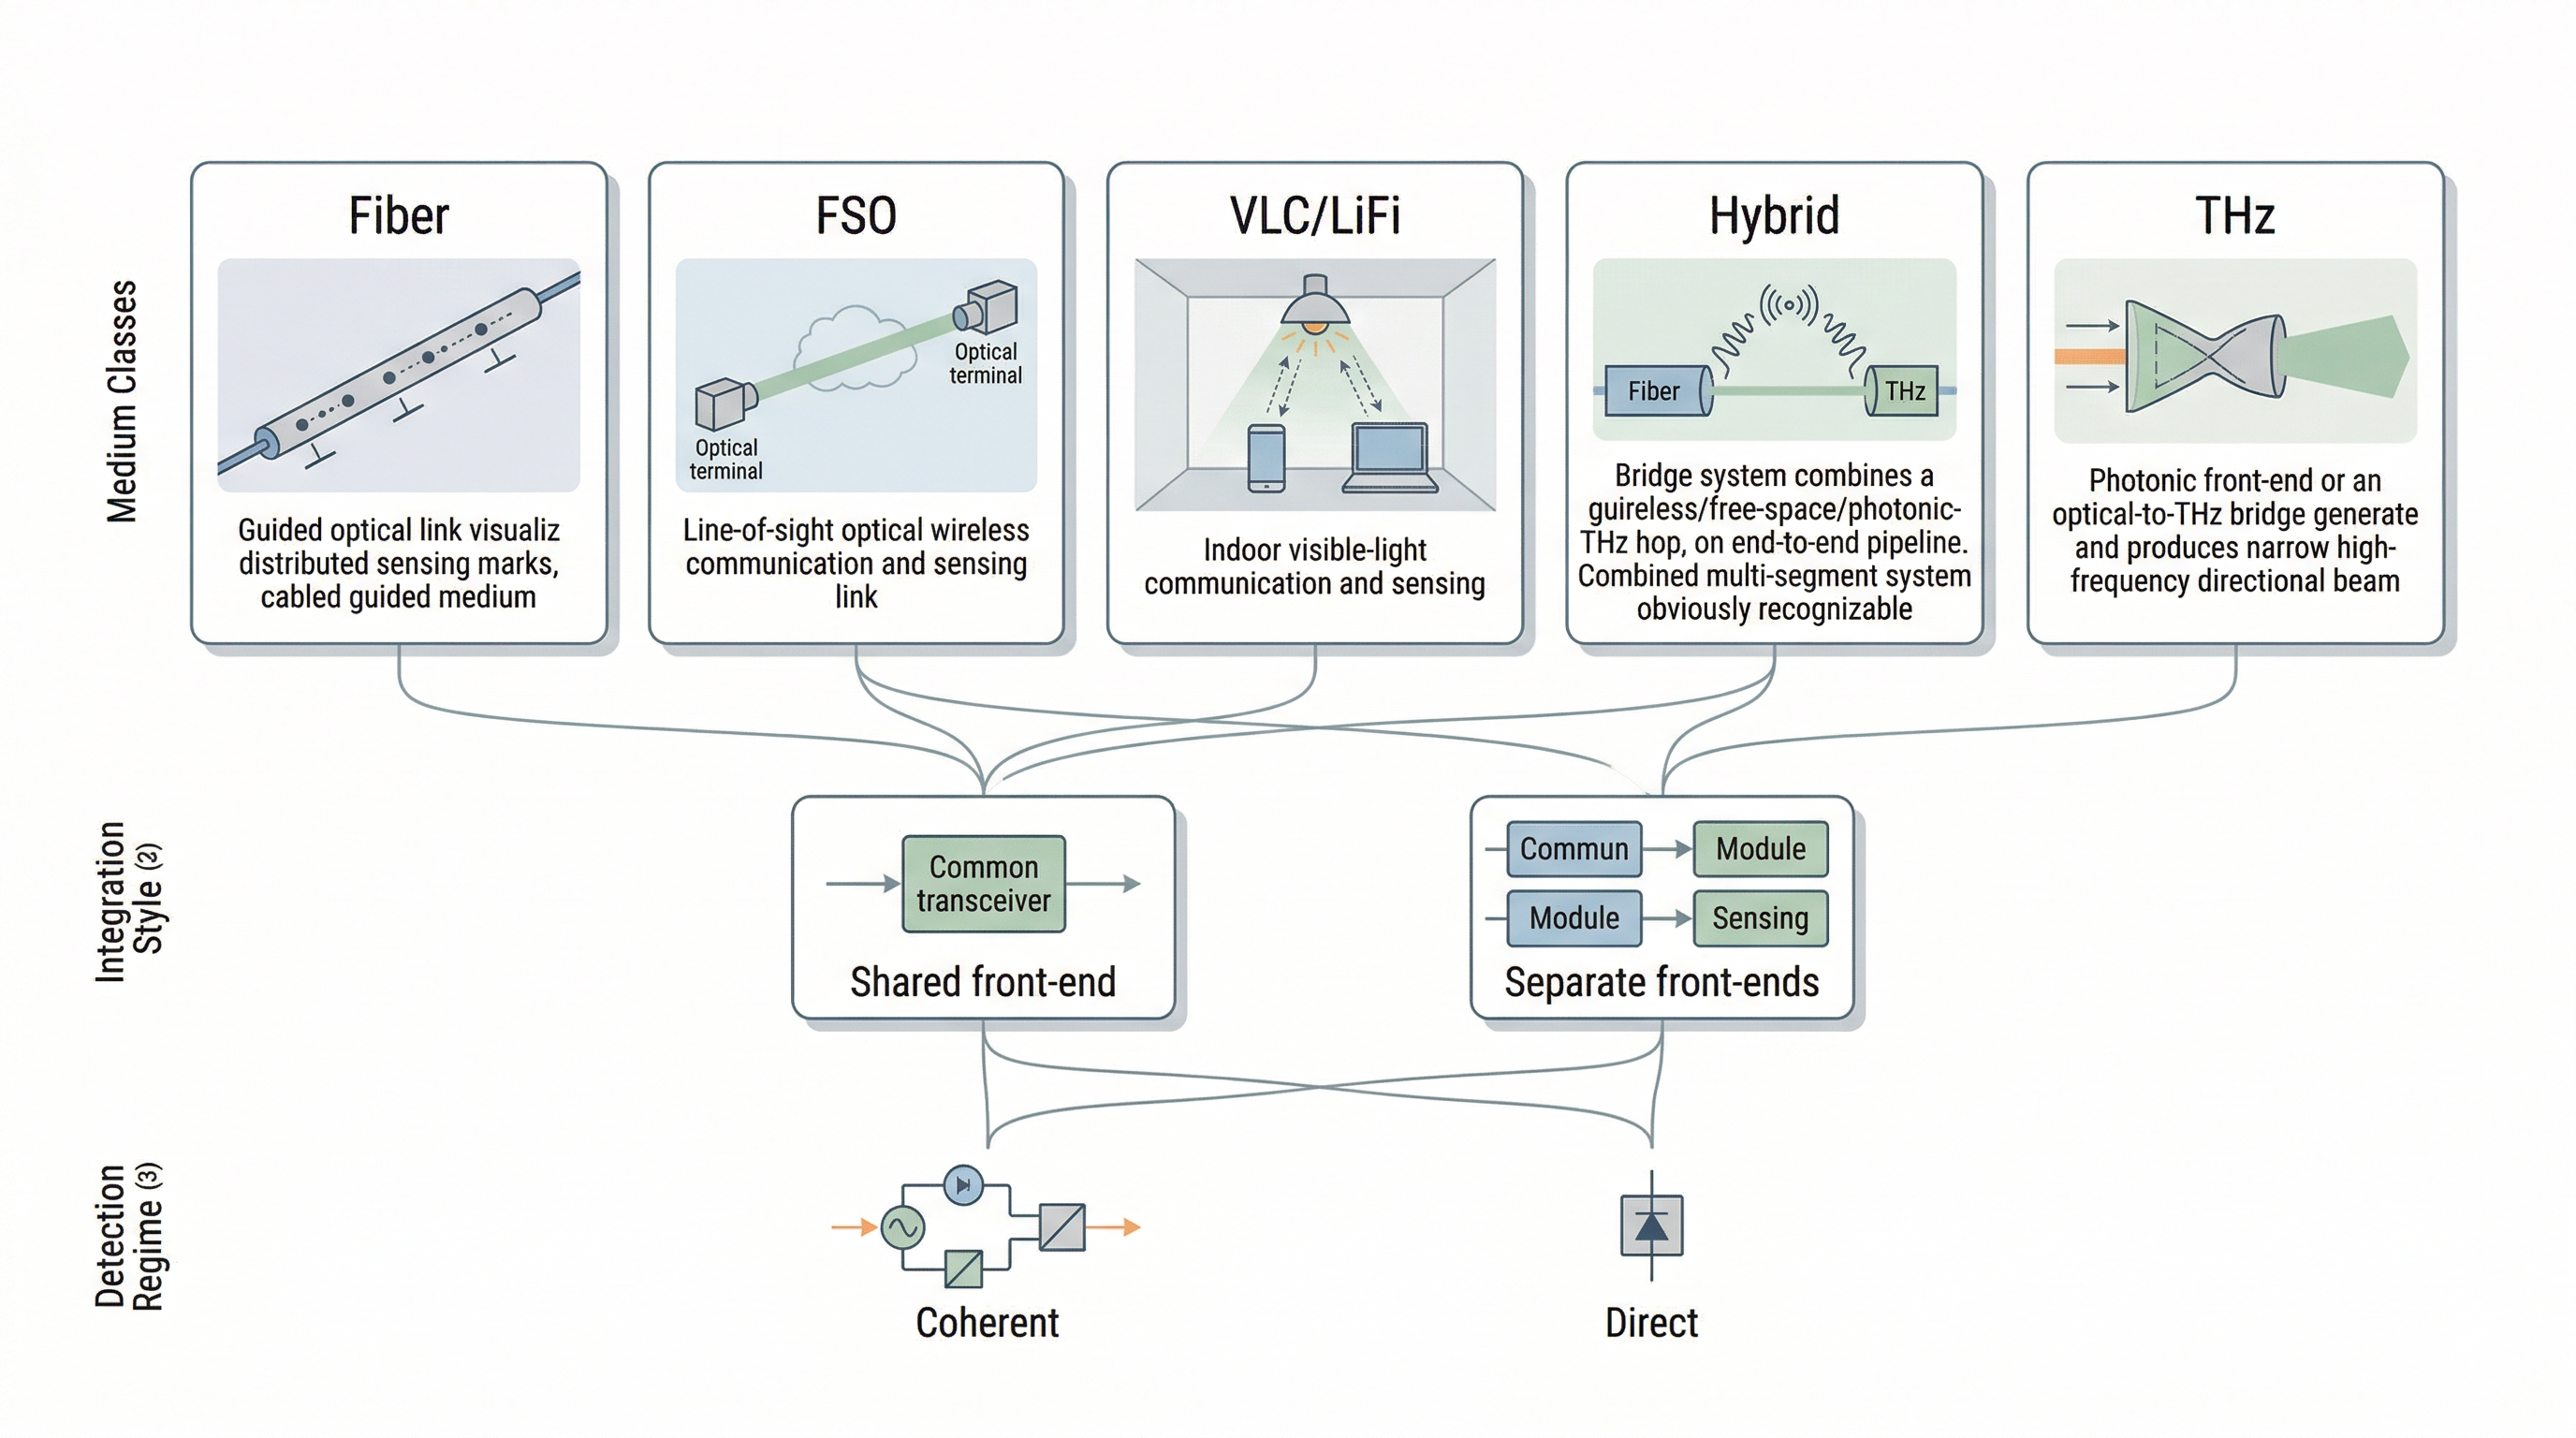
\includegraphics[width=\linewidth,trim=0.8cm 0.7cm 0.8cm 1.1cm,clip]{figures/fig_iv_1.png}
    \caption{Reader-facing semantic taxonomy map for O-ISAC. The figure visualizes fiber, FSO, VLC/LiFi, hybrid, and THz-linked classes and links them to integration style and detection regime. Its role is explanatory rather than rank-implying, preceding the denser synthesis in Table~\ref{tab:taxonomy_clusters} and Fig.~\ref{fig:fig_iv_2}.}
    \label{fig:fig_iv_1}
\end{figure*}

Section II governance remains binding at figure level: no implicit OSNR-to-SNR substitution is allowed without explicit receiver/noise modeling, and no resolution-versus-accuracy aliasing is admitted when comparing taxonomy states \cite{O_ISAC_021,O_ISAC_039,O_ISAC_077,O_ISAC_132,O_ISAC_061}.

\subsubsection{Taxonomy Table}
Table~\ref{tab:taxonomy_clusters} complements Fig.~\ref{fig:fig_iv_1} by encoding clustered patterns rather than one-row-per-paper listings, so Sections IV--VI can reference stable taxonomy clusters with explicit comparability guards.

\begin{table*}[!t]
\caption{Taxonomy Summary Views and Cluster-Level Synthesis Contract}
\label{tab:taxonomy_clusters}
\centering
\footnotesize
\begin{tabularx}{\textwidth}{@{}%
>{\raggedright\arraybackslash}p{1.55cm}
>{\raggedright\arraybackslash}X
>{\raggedright\arraybackslash}X
>{\raggedright\arraybackslash}X
>{\raggedright\arraybackslash}X
>{\raggedright\arraybackslash}X
>{\raggedright\arraybackslash}X
>{\raggedright\arraybackslash}p{2.2cm}
@{}}
\toprule
\textbf{\shortstack{Taxonomy\\Cluster}} &
\textbf{\shortstack{Dominant Deployment\\Scenario}} &
\textbf{\shortstack{Integration\\Mechanism}} &
\textbf{\shortstack{Detection /\\Observability}} &
\textbf{\shortstack{Representative\\Sensing Tasks}} &
\textbf{\shortstack{Primary Communication\\Metrics}} &
\textbf{\shortstack{Primary Sensing\\Metrics}} &
\textbf{\shortstack{Representative\\References}} \\
\midrule

Fiber-guided O-ISAC cluster &
Long-reach cabled links with distributed monitoring overlays &
Shared front-end dominant &
Coherent-leading with a direct subset &
Ranging primary, with vibration concentration and a fault-localization tail &
BER, FEC margin, and communication robustness &
Spatial granularity/ranging and vibration indicators &
\cite{O_ISAC_006,O_ISAC_041,O_ISAC_013} \\

FSO wireless optical cluster &
Line-of-sight outdoor and inter-building optical links &
Shared front-end with a non-negligible separate-front-end subset &
Mixed direct/coherent regime &
Ranging dominant, with a small localization tail &
BER, outage, and spectral efficiency &
Range estimation and resolution-class indicators &
\cite{O_ISAC_021,O_ISAC_023,O_ISAC_199} \\

VLC/LiFi indoor cluster &
Illumination-constrained indoor access and positioning &
Shared front-end dominant &
Direct-detection and intensity-only dominant &
Ranging with a strong localization concentration &
Throughput, BER, and link reliability &
Localization error and ranging metrics &
\cite{O_ISAC_068,O_ISAC_039,O_ISAC_009} \\

Hybrid bridge cluster &
Fiber-wireless and photonic-THz bridging pipelines &
Shared front-end dominant &
Near-balanced coherent/direct mix with residual labels &
Ranging dominant with a multi-task tail &
Throughput and BER under cross-link coupling &
Range/localization and task-specific errors &
\cite{O_ISAC_077,O_ISAC_010,O_ISAC_190} \\

Residual low-support cluster &
\parbox[t]{\linewidth}{\raggedright\scriptsize Specialized or emerging\\ deployment cases} &
Mixed mechanisms &
\parbox[t]{\linewidth}{\raggedright\scriptsize Mostly direct, with\\ sparse alternatives} &
\parbox[t]{\linewidth}{\raggedright\scriptsize Heterogeneous\\ low-support tasks} &
\shortstack{Context-\\dependent} &
\shortstack{Context-\\dependent} &
\cite{O_ISAC_070,O_ISAC_056} \\
\bottomrule
\end{tabularx}
\end{table*}

Ambiguity remains explicit at cluster level: the same 84 flagged records are retained and interpreted conservatively when aliasing or plane ambiguity remains unresolved. Fig.~\ref{fig:fig_iv_2} then complements Table~\ref{tab:taxonomy_clusters} with a reader-facing specialization view, making the global dominance of ranging and the secondary localization, vibration, and multi-task tails easier to recognize before returning to the denser table-level synthesis \cite{O_ISAC_006,O_ISAC_068,O_ISAC_077,O_ISAC_039}.


\begin{figure*}[!t]
    \centering
    
\includegraphics[width=\linewidth]{figures/fig_iv_2.png}
    \caption{Reader-facing medium-task specialization view for O-ISAC. The figure highlights how dominant medium classes connect to representative sensing emphases, including ranging, VLC/LiFi localization, fiber vibration monitoring, and hybrid multi-task breadth, without implying that prevalence means superiority. It complements the denser cluster-level synthesis in Table~\ref{tab:taxonomy_clusters}.}
    \label{fig:fig_iv_2}
\end{figure*}

\section{COMMUNICATION-SENSING TRADEOFF SYNTHESIS}

Building on the Section II metric-governance contract and the Section IV taxonomy state, Section V converts broad study-level evidence into governed, scenario-level quantitative interpretation. It is therefore the manuscript's admissibility-controlled synthesis layer: Section IV determines which records are structurally comparable, and Section V asks what remains quantitatively interpretable once plane and metric-role consistency are enforced.

\subsection{Communication Metrics}
Section V-A works on governed scenario records rather than raw study counts. Communication metrics are scoped to reported communication rate ($R$) and link-quality indicators, with strict separation between optical-plane OSNR and electrical-plane SNR/ESNR because the two are measured at different receiver-chain stages. Table~\ref{tab:comm_metrics} summarizes the resulting plane-aware coverage.

\begin{table*}[!t]
\caption{Governed Communication-Metric Coverage and Plane-Aware Availability}
\label{tab:comm_metrics}
\centering
\footnotesize
\begin{tabularx}{\textwidth}{@{}%
>{\raggedright\arraybackslash}p{2.15cm}
>{\raggedright\arraybackslash}X
>{\raggedright\arraybackslash}X
>{\raggedright\arraybackslash}p{2.2cm}
>{\raggedright\arraybackslash}X
@{}}
\toprule
\textbf{Communication Metric} &
\textbf{Raw Scenario Coverage} &
\textbf{Governed Usable Coverage} &
\textbf{\shortstack{Governed Range /\\Median}} &
\textbf{Interpretation Note} \\
\midrule

Rate ($R$) &
197/225 records; 194/220 papers &
33 rate-bearing records within 53 governed scenarios &
25 Mbps to 448 Gbps; median 10 Gbps &
Supports comparative communication synthesis only with explicit support-size caveats \\

Electrical-plane SNR &
190/225 records; 186/220 papers &
20/53 governed records &
7--22 dB; median 10 dB &
The only governed quality indicator that survives filtering across more than one medium slice \\

Optical-plane OSNR &
169/225 records; 166/220 papers &
0/53 governed records &
-- &
\parbox[t]{\linewidth}{\raggedright\scriptsize All OSNR-bearing records are blocked\\ by plane mixing in this release} \\
\bottomrule
\end{tabularx}
\end{table*}

Before governance filtering, communication reporting appears broad: the 225-point trade-off set includes rate in 197 records, electrical-plane SNR in 190, and optical-plane OSNR in 169. After the Section II filter, however, only 53/225 scenarios remain usable, 172 are blocked, and 169 papers lose all scenarios. The dominant blocker is metric-plane mixing (169 records), followed by $\Delta z$-to-$\Delta r_{\min}$ aliasing (19 records, with 16 overlapping both flags). Within the governed subset, rate-bearing records are concentrated in hybrid (17) and cabled fiber (12), yielding medians of 10 Gbps and 28.5 Gbps, respectively; the remaining media are sparse and should be read as anchors rather than distributions. Electrical-plane SNR survives in only 20 governed records, while governance-usable OSNR drops to zero, so Section V-A can support electrical-plane quality remarks but not optical-plane cross-medium comparisons. CRQ-linked comments are likewise bounded to the 20 eligible records, dominated by hybrid (14) and cabled fiber (4). The same pattern explains the section's conservatism overall: the governance audit reports 299 MAJOR violations across 169 papers, including 261 metric-plane and 38 metric-aliasing violations, so communication synthesis remains intentionally selective rather than coverage-maximizing.

\subsection{Sensing Metrics}
Section V-B keeps the same governed scenario scope but reorganizes sensing evidence by function rather than by lexical surface form. $\Delta r_{\min}$ represents physical resolution, $\sigma_r$ estimator-level accuracy, CRB bound-level context, and $\Delta z$ fiber spatial granularity; these roles are not interchangeable, so Table~\ref{tab:sensing_metrics} reports them separately and Fig.~\ref{fig:fig_v_1} later preserves distinct resolution and accuracy layers.


\begin{table*}[!t]
\caption{Governed Sensing-Metric Coverage by Functional Role}
\label{tab:sensing_metrics}
\centering
\footnotesize
\begin{tabularx}{\textwidth}{@{}%
>{\raggedright\arraybackslash}p{2.35cm}
>{\raggedright\arraybackslash}X
>{\raggedright\arraybackslash}X
>{\raggedright\arraybackslash}p{2.2cm}
>{\raggedright\arraybackslash}X
@{}}
\toprule
\textbf{Sensing Role} &
\textbf{Raw Scenario Coverage} &
\textbf{Governed Usable Coverage} &
\textbf{\shortstack{Governed Range /\\Median}} &
\textbf{Interpretation Note} \\
\midrule

Resolution ($\Delta r_{\min}$-eligible) &
173/225 eligible records; 170/220 papers &
20/173 eligible records &
0.0025 m to 15 m; median 0.0397 m &
Physical resolution is retained only on the role-consistent governed subset \\

Accuracy ($\sigma_r$) &
186/225 records; 183/220 papers &
16/186 records &
0.001 m to 1000 m; median 0.0575 m &
Estimator-level accuracy remains distinct from resolution and is not pooled with $\Delta r_{\min}$ \\

CRB &
148/225 records; 145/220 papers &
0/148 records &
-- &
Bound-level reporting remains contextual only after governance filtering \\

Fiber spatial granularity ($\Delta z$) &
161/225 records; 158/220 papers &
0/161 records &
-- &
\parbox[t]{\linewidth}{\raggedright\scriptsize $\Delta z$ is retained as fiber-specific context\\ and is never substituted for $\Delta r_{\min}$} \\
\bottomrule
\end{tabularx}
\end{table*}



Before governance filtering, sensing coverage is broad: across 225 scenario points, $\Delta r_{\min}$ appears in 195 records, $\Delta r_{\min}$-eligible reporting in 173, $\sigma_r$ in 186, CRB in 148, and $\Delta z$ in 161, with similarly high paper-level coverage. After filtering, however, only 53/225 scenarios remain usable overall. At role level, only 20/173 $\Delta r_{\min}$-eligible records and 16/186 $\sigma_r$ records survive, while both CRB and $\Delta z$ fall to zero usable entries. The exclusion pattern is highly structured rather than random: 151/153 blocked $\Delta r_{\min}$-eligible records, 169/170 blocked $\sigma_r$ records, and 147/148 blocked CRB records are plane-mixed. Table~\ref{tab:sensing_metrics} therefore separates reported coverage from governance-usable coverage because raw prevalence overstates comparative readiness.

Within the governed subset, $\Delta r_{\min}$-eligible points are concentrated in hybrid (14) and cabled fiber (4), with single anchors in wireless FSO and terahertz; across all usable points, $\Delta r_{\min}$ spans 0.0025--15 m with a median of 0.0397 m. Estimator-level accuracy is even sparser: only 16 usable records report $\sigma_r$ (hybrid 8, cabled fiber 7, terahertz 1), spanning 0.001--1000 m with a median of 0.0575 m, and only 13 usable records contain both $\Delta r_{\min}$ and $\sigma_r$. This asymmetry is why Fig.~\ref{fig:fig_v_1} keeps separate resolution and accuracy panels. CRB and $\Delta z$ remain contextual only, because neither survives governance filtering; OSNR is likewise absent from the usable sensing subset, whereas electrical-plane SNR remains available in 12/20 $\Delta r_{\min}$-eligible and 14/16 $\sigma_r$ records. The same conservatism also matches the qualitative trade-off record: DIRECT articulation exists, but it remains a minority pattern relative to total mention volume, and the 299 MAJOR governance violations across 169 papers continue to limit synthesis-ready support.


\subsection{Sensing-Communication Trade-off}
Section V-C is the synthesis core of the section: it converts the governed metric subsets into operating-cloud and frontier-style views without relaxing the Section II contract. Rate-versus-resolution is interpreted through rate and $\Delta r_{\min}$, rate-versus-accuracy through rate and $\sigma_r$, while CRB remains bound-level context and $\Delta z$ is never used as a surrogate for $\Delta r_{\min}$. Fig.~\ref{fig:fig_v_1} therefore keeps the resolution and accuracy layers separate, and Fig.~\ref{fig:fig_v_2} zooms into the CRQ-valid frontier subset.

\begin{figure*}[!t]
    \centering
    
\includegraphics[width=\linewidth]{figures/fig_v_1.png}
    \caption{Reader-facing governed operating clouds for Section V. The left panel shows rate-versus-$\Delta r_{\min}$ and the right panel rate-versus-$\sigma_r$ after admissibility filtering. Gray points denote role-conditioned raw context, colored points denote governance-usable records, and the separated panels keep physical resolution distinct from estimator-level accuracy.}
    \label{fig:fig_v_1}
\end{figure*}

The full trade-off table contains 225 scenario points from 220 papers, but the governed subset is much smaller: only 20 points support rate-plus-$\Delta r_{\min}$ interpretation and 16 support rate-plus-$\sigma_r$, with only 13 supporting the full triplet. This contraction is not cosmetic; it determines the admissible evidence for trade-off inference. Labels remain useful narrative cues, but dimensional interpretation is grounded in governed metric availability rather than label strings alone. The governed operating region is still numerically informative: rate spans 25 Mbps to 448 Gbps (median 10 Gbps), $\Delta r_{\min}$ spans 0.0025--15 m (median 0.0397 m), and $\sigma_r$ spans 0.001--1000 m (median 0.0575 m). Coupling-mode coverage is likewise asymmetric, with \texttt{resource\_division} dominant in both the raw and governed sets.

CRQ filtering makes the admissibility compression even clearer. The point taxonomy is 225 total points, 170 CRQ-candidate points, 20 CRQ-valid points, and only 2 Pareto points. The 20 valid points are distributed across hybrid (14), cabled fiber (4), terahertz (1), and wireless FSO (1), with CRQ spanning $6.67 \times 10^8$ to $4.8 \times 10^{13}$ bps/m and a median of $4.33 \times 10^{10}$ bps/m. Because the frontier itself contains only one hybrid and one wireless FSO point, Fig.~\ref{fig:fig_v_2} should be read as a bounded illustrative frontier rather than a stable design envelope. The same caveat applies to measurement-plane conditioning: electrical-plane SNR remains available in part of the governed subset, but governance-usable OSNR remains absent throughout.

\begin{figure*}[!t]
    \centering
    
\includegraphics[width=\linewidth]{figures/fig_v_2.png}
    \caption{Reader-facing sparse frontier for the CRQ-valid subset of Section V. Faint markers denote the 20 governance-usable points and outlined markers the 2 nondominated Pareto points. The figure is therefore a bounded frontier illustration rather than a full-cloud or modality-ranking view.}
    \label{fig:fig_v_2}
\end{figure*}

Trade-off-language extraction is consistent with this conservatism: explicit trade-off reasoning exists, but DIRECT articulation remains a minority pattern relative to total mention volume. The same 299 MAJOR governance violations across 169 papers therefore remain central to interpretation in V-C, because they explain much of the candidate-to-valid compression and the sparsity of the Pareto set.



\subsection{Comparative Analysis: Fiber vs Wireless}
Section V-D keeps the same governed scenario scope but changes the question from ``what is available?'' to ``what can be compared responsibly?''. Medium labels remain exactly as normalized in Section IV, hybrid is retained as a bridge class rather than forced into either endpoint, and Table~\ref{tab:comparative_slices} is the primary comparative anchor.


\begin{table*}[!t]
\caption{Governed Fiber, Wireless, and Hybrid Slices}
\label{tab:comparative_slices}
\centering
\footnotesize
\begin{tabularx}{\textwidth}{@{}%
>{\raggedright\arraybackslash}p{2.0cm}
>{\raggedright\arraybackslash}p{1.65cm}
>{\raggedright\arraybackslash}p{1.7cm}
>{\raggedright\arraybackslash}p{1.7cm}
>{\raggedright\arraybackslash}p{1.6cm}
>{\raggedright\arraybackslash}p{2.0cm}
>{\raggedright\arraybackslash}X
@{}}
\toprule
\textbf{Comparative Slice} &
\textbf{\shortstack{Governed Points\\(Papers)}} &
\textbf{Median Rate} &
\textbf{Median $\Delta r_{\min}$} &
\textbf{Median $\sigma_r$} &
\textbf{\shortstack{Median CRQ\\(Eligible Only)}} &
\textbf{Coupling Composition} \\
\midrule

Fiber (cabled fiber slice) &
15 (13) &
28.5 Gbps (\texttt{n\_rate=12}) &
5.5 m (\texttt{n=4}) &
0.1 m (\texttt{n=7}) &
$5.50 \times 10^9$ bps/m (\texttt{n=4}) &
\texttt{resource\_division} 13; \texttt{joint\_waveform} 2 \\

Wireless (pooled wireless slice) &
9 (9) &
1 Gbps (\texttt{n\_rate=3}) &
0.0025 m (\texttt{n=1}) &
-- &
$4.80 \times 10^{13}$ bps/m (\texttt{n=1}) &
\texttt{resource\_division} 5; \texttt{joint\_waveform} 4 \\

Hybrid bridge slice &
27 (27) &
10 Gbps (\texttt{n\_rate=17}) &
0.019075 m (\texttt{n=14}) &
0.01 m (\texttt{n=8}) &
$8.83 \times 10^{10}$ bps/m (\texttt{n=14}) &
\parbox[t]{\linewidth}{\raggedright\scriptsize resource\_division 19;\\ joint\_waveform 6;\\ unlabeled 2} \\
\bottomrule
\end{tabularx}
\end{table*}




The contraction from raw to governed evidence directly shapes what can be compared. The raw trade-off set contains 225 scenario points across 12 medium labels, but governance filtering retains only 53, distributed mainly across hybrid (27), cabled fiber (15), and smaller wireless slices. Within that governed set, fiber contributes 15 points from 13 papers, wireless 9 points from 9 papers, and hybrid 27 points from 27 papers. Metric completeness is asymmetric: fiber contributes 12 rate values, 4 $\Delta r_{\min}$ values, and 7 $\sigma_r$ values; wireless contributes 3, 1, and 0; hybrid contributes 17, 14, and 8. Table~\ref{tab:comparative_slices} should therefore be read as a constrained synthesis over a reduced admissible set rather than as a mirror of raw-corpus prevalence.

The governed medians suggest different operating emphases, but not universal superiority claims. Fiber shows a median rate of 28.5 Gbps, wireless 1 Gbps, and hybrid 10 Gbps, yet the wireless slice is structurally unstable because it is sparse and heterogeneous. Sensing-side comparison is even more asymmetric: fiber has median $\Delta r_{\min}=5.5$ m and median $\sigma_r=0.1$ m, wireless has only one governed $\Delta r_{\min}$ value and no governed $\sigma_r$, and hybrid supports both metrics with medians of 0.019075 m and 0.01 m. CRQ comparison is similarly bounded to the 20 eligible points, while electrical-plane SNR remains available only for fiber, hybrid, and one wireless anchor. V-D is therefore intentionally conservative: it preserves comparison where support exists, keeps hybrid explicit, and treats sparse slices as non-ranking evidence.





\subsection*{Section V closeout synthesis}
Section V therefore closes on a deliberately conservative conclusion. Frontier-style interpretation is bounded by three nested evidence layers: the raw 225-point cloud, the 53-point governed cloud, and the 20-point CRQ-valid subset from which only 2 Pareto points are selected. Those Pareto points are illustrative rather than definitive, and the absence of some media from the frontier should be read as sparse support, not inferiority. The practical implication is straightforward: decision-stage claims should be anchored in CRQ-valid evidence, operating-point discussions should report both $\Delta r_{\min}$ and $\sigma_r$ whenever possible, and medium, coupling mode, and measurement plane should remain attached to every frontier-style interpretation.




\section{ENABLING TECHNOLOGIES AND SYSTEM-LEVEL CO-DESIGN FOR OPTICAL ISAC}

Section VI asks which enablers make O-ISAC deployable under realistic channel, control, and benchmarking constraints. Across the current evidence base, OPA, ORIS, robustness-aware optimization, and network coordination recur as coupled design levers rather than isolated modules \cite{O_ISAC_008,O_ISAC_023,O_ISAC_061,O_ISAC_091,O_ISAC_098,O_ISAC_112,O_ISAC_127}. Accordingly, the anchors promised in Section I, namely ORIS, OPA, photonics-assisted signal generation, and machine learning integration, are interpreted here through system-level feasibility rather than as a component catalog. We therefore preserve the Section II measurement guards, reuse the Section IV taxonomy framing, and emphasize design opportunity and constraint structure wherever study-level maturity remains limited.

Throughout this section, we use \textbf{ORIS (Optical Reconfigurable Intelligent Surface)} as the canonical umbrella term for optical RIS-style programmable surfaces. One shared notation block is retained so that OPA steering, ORIS-assisted links, robustness constraints, and multi-user optimization can be discussed without symbol drift across subsections (Table~\ref{tab:section6_notation}).




\begin{table}[!t]
\caption{Unified Notation for Section VI}
\label{tab:section6_notation}
\centering
\footnotesize
\begin{tabularx}{\columnwidth}{@{}>{\raggedright\arraybackslash}p{1.85cm}>{\raggedright\arraybackslash}X>{\raggedright\arraybackslash}p{1.55cm}@{}}
\toprule
\textbf{Symbol} & \textbf{Meaning} & \textbf{Used in} \\
\midrule
$x(t)$ & Optical transmit waveform or equivalent sampled signal & VI-C, VI-E \\
$\ell$ & Link distance in benchmark-scenario disclosure & VI-D \\
$\bar P$ & Average optical power budget & VI-C, VI-D \\
$P_{\max}$ & Peak optical power budget & VI-C, VI-D \\
$H$ & End-to-end channel coefficient or gain & VI-B \\
$H_l$ & Deterministic or path-loss component of $H$ & VI-B \\
$H_a$ & Atmospheric or medium-turbulence component of $H$ & VI-B \\
$H_p$ & Pointing or misalignment component of $H$ & VI-B \\
$\gamma$ & Instantaneous reliability proxy evaluated on a fixed detection plane; no cross-plane substitution is implied & VI-B, VI-E \\
$\gamma_{\text{th}}$ & Reliability threshold for outage control & VI-B \\
$\varepsilon$ & Allowed outage-probability target & VI-B, VI-C \\
$m_{\text{res}}$ & Role-consistent resolution or granularity metric & VI-D \\
$m_{\text{acc}}$ & Empirical sensing accuracy metric & VI-D \\
$m_{\text{bnd}}$ & Bound-type sensing-metric family & VI-D \\
$\sigma_r$ & Estimator-dependent sensing accuracy metric when reported & VI-D \\
$\Theta$ & ORIS diagonal response matrix & VI-A, VI-C, VI-E, VI-F \\
$\beta_n$ & ORIS amplitude coefficient of element $n$ & VI-A \\
$\theta_n$ & ORIS phase of element $n$ & VI-A, VI-E \\
$Q$ & Number of phase-quantization levels & VI-A, VI-E \\
$\mathbf{w}_k$ & Beamforming vector for user $k$ & VI-C, VI-E \\
$\mathrm{SINR}_k$ & User-$k$ communication quality metric & VI-E \\
$\mathrm{CRB}$ & Bound-type sensing metric; not interchangeable with empirical accuracy metrics & VI-C, VI-D, VI-E, VI-F \\
\bottomrule
\end{tabularx}
\end{table}




\begin{quote}
\textbf{Model VI-U (Unified Channel/Signal Model).}

\begin{equation}
y_k = \left(h_{d,k} + \mathbf{h}_{r,k}^{T}\Theta\mathbf{g}\right)x + n_k
\end{equation}
\begin{equation}
\Theta = \operatorname{diag}\!\left(\beta_n e^{j\theta_n}\right)
\end{equation}
\begin{equation}
\theta_n \in \left\{0,\frac{2\pi}{Q},\ldots,\frac{2\pi(Q-1)}{Q}\right\}
\end{equation}

Model VI-U is a compact abstraction reused across VI-A, VI-C, VI-E, and VI-F for notation consistency \cite{O_ISAC_061,O_ISAC_091,O_ISAC_098,O_ISAC_127}.
\end{quote}

\subsection{Programmable Optical Enablers}

Programmable optical enablers matter because they convert optical propagation from a mostly fixed channel into a controllable channel. OPA studies expose transmit-side beam agility, angular selectivity, and joint waveform support, whereas ORIS studies expose environment-side path shaping, alignment assistance, and blockage mitigation through reflected or reconstructed paths \cite{O_ISAC_008,O_ISAC_061,O_ISAC_091,O_ISAC_098,O_ISAC_112}. This distinction is important: OPA and ORIS should be written as complementary control authorities rather than as interchangeable technologies.

A compact steering anchor for OPA is
\begin{equation}
AF(\theta)=\sum_{m=0}^{M-1} a_m\exp\!\left(j\left(kdm\sin\theta+\phi_m\right)\right)
\end{equation}
\begin{equation}
\phi_m^{\star}=-kdm\sin\theta_0
\end{equation}
which steers the main lobe toward $\theta_0$ under accurate phase control \cite{O_ISAC_008,O_ISAC_061,O_ISAC_091}. In practice, finite receiver FoV, grating-lobe behavior, insertion loss, and channel impairments prevent ideal steering gains from translating directly into reproducible O-ISAC gains \cite{O_ISAC_061,O_ISAC_091,O_ISAC_098}.

PIC, programmable photonics, and photonics-assisted signal generation are treated here as supporting substrates beneath OPA/ORIS rather than as a detached maturity tier. Their main value is explanatory: they clarify packaging, integration pathway, and hardware-stack feasibility, but measurable O-ISAC gains are still anchored more directly to the primary programmable-surface and beam-steering narratives. Prevalence wording therefore remains conservative, as summarized in Table~\ref{tab:vi_a_enablers}.



\begin{table*}[!t]
\caption{Section VI-A Comparison of Programmable Optical Enabler Families}
\label{tab:vi_a_enablers}
\centering
\footnotesize
\begin{tabularx}{\textwidth}{@{}%
>{\raggedright\arraybackslash}p{2.0cm}
>{\raggedright\arraybackslash}X
>{\raggedright\arraybackslash}X
>{\raggedright\arraybackslash}X
@{}}
\toprule
\textbf{Enabler Family} &
\textbf{Primary Control Role in O-ISAC} &
\textbf{Strongest Evidence Posture in This Review} &
\textbf{Main Deployment Constraints} \\
\midrule

OPA &
Transmit-side beam agility, angular selectivity, and joint communication--sensing steering &
Primary evidence core; Section I contribution count includes 7 study-level papers, whereas broader structured traces are used only as supporting context &
Grating lobes, finite receiver FoV, insertion loss, and sensitivity to atmospheric or channel loss \\

ORIS &
Environment-side path shaping, blockage mitigation, alignment assistance, and NLoS reconstruction &
Primary evidence core; Section I contribution count includes 8 study-level papers, whereas broader structured traces are used only as supporting context &
Refresh latency, attenuation, phase quantization, coherence-time mismatch, and control overhead \\

PIC / programmable photonics &
Integration substrate for packaging, routing, and scalable optical control &
Qualitative/supporting only; used to explain how controllable optics may be integrated, rather than to claim mature O-ISAC adoption &
Calibration burden, packaging complexity, insertion loss, and hardware-stack dependence \\

Photonics-assisted signal generation / photonic-THz bridge &
Source and distribution pathway for hybrid optical--wireless control chains &
Bridge evidence only; relevant for hybrid-system interpretation, but not a standalone maturity claim in Section VI-A &
Stage-aware modeling, cross-plane reporting, and front-end chain complexity \\
\bottomrule
\end{tabularx}
\end{table*}





Evidence note: OPA/ORIS prevalence wording follows the strict study-level view used in Section I; broader traces remain contextual, and Table~\ref{tab:vi_a_enablers} together with Fig.~\ref{fig:fig_vi_1} summarize the enabler landscape without inflating adoption claims.

\begin{figure*}[!t]
    \centering
    
\includegraphics[width=\linewidth]{figures/fig_vi_1.jpg}
    \caption{Section VI enabler landscape across medium classes. OPA and ORIS are the primary programmable-enabler evidence cores, whereas PIC, photonic generation, and programmable photonics remain supporting substrate families; medium-wise concentrations are shown without turning contextual traces into maturity claims.}
    \label{fig:fig_vi_1}
\end{figure*}


\textbf{VI-A takeaway.} OPA evidence is strongest on beam agility and communication-sensing coupling, while ORIS evidence is strongest on alignment robustness and NLoS support; quantized control, insertion loss, and refresh latency remain the main bottlenecks. VI-A therefore supports programmable optics as a promising but unevenly validated control space, with PIC and photonic-integration themes serving mainly as packaging context. The next question is whether that controllability survives the actual impairment profile of the optical channel.

\subsection{Channel Impairments and Robustness}

Robustness is a first-order concern in O-ISAC because the same optical channel impairments degrade communication reliability and sensing fidelity together. Across FSO, VLC/LiFi, and hybrid optical settings, the literature repeatedly models end-to-end gain as a composition of deterministic loss, atmospheric or medium turbulence, and pointing or alignment components \cite{O_ISAC_023,O_ISAC_035,O_ISAC_061,O_ISAC_098,O_ISAC_199}. Guided-fiber cases remain important, but they require different impairment abstractions and should not be silently collapsed into the same wireless robustness template. This is the point where enabler value becomes conditional: a programmable surface or beam-steering mechanism is only useful insofar as it remains effective under the dominant impairment regime.

A compact robustness anchor is
\begin{equation}
H=H_l H_a H_p
\end{equation}
\begin{equation}
P_{\text{out}}=\Pr\!\left(\gamma(H)<\gamma_{\text{th}}\right)\le \varepsilon
\end{equation}

This chance-constrained view links physical impairment statistics directly to reliability targets and is consistent with quantile-robust formulations already used in optical ISAC optimization studies \cite{O_ISAC_023,O_ISAC_061,O_ISAC_091}. Here $\gamma$ must stay tied to one declared detection plane per scenario; the expression does not permit implicit OSNR-to-electrical-SNR conversion or blind pooling of coherent and direct observations. Practical mitigation then combines design-time robustness with runtime adaptation through tracking, refresh control, environment-aware reconfiguration, and fallback or diversity mechanisms \cite{O_ISAC_098,O_ISAC_112,O_ISAC_127,O_ISAC_199}.

The prose here must stay medium-aware: turbulence and weather attenuation dominate many FSO and hybrid scenarios, finite FoV and geometry dominate many VLC scenarios, and control latency cuts across most programmable optical platforms. Section VI therefore cannot write ``robustness'' as if one impairment model covered all optical modalities equally well.

\textbf{VI-B takeaway.} Current literature supports robustness-aware optical design, but outage definitions and confidence reporting remain heterogeneous. The review-level lesson is that controllability becomes meaningful only after impairment-aware conditioning, which naturally leads to joint optimization under explicit reliability constraints in VI-C.

\subsection{Joint Co-Design and Resource Optimization}

Joint co-design is required because waveform, beam, power, and ORIS controls share physical constraints. In IM/DD implementations, feasible signaling must satisfy nonnegativity and optical power bounds, while coherent or programmable settings add quantization, steering, and update constraints \cite{O_ISAC_009,O_ISAC_023,O_ISAC_054,O_ISAC_061,O_ISAC_091,O_ISAC_127}. Model VI-U is useful here because it keeps transmitter, ORIS, and sensing terms in one variable structure.

A minimal feasible-set and objective anchor is
\begin{equation}
\begin{split}
\mathcal U=\{x(t):x(t)\ge 0,\;\mathbb{E}[x(t)]\le \bar P,\\
\qquad \max_t x(t)\le P_{\max}\}
\end{split}
\end{equation}
\begin{equation}
\begin{split}
\max_{\mathbf{w},\Theta,\,x\in\mathcal U}\;&\alpha R(\mathbf{w},\Theta)\\
&-(1-\alpha)\,\mathrm{CRB}(\mathbf{w},\Theta),\quad \alpha\in[0,1]
\end{split}
\end{equation}

The weight $\alpha$ sets the communication-sensing operating point and can be extended with reliability and latency constraints when channel dynamics are explicit \cite{O_ISAC_023,O_ISAC_061,O_ISAC_091,O_ISAC_127}. Within this subsection, $\mathrm{CRB}$ is retained as a bound-type sensing term rather than an empirical accuracy or resolution proxy. The evidence supports a structured control space, but adoption claims should remain modest: strong study-level co-design demonstrations are fewer than the broader metric traces, and many reported formulations remain exemplar-driven rather than reproducibly benchmarked.

\textbf{VI-C takeaway.} Evidence is strongest for structured optimization in a limited set of well-specified exemplars. The main gap is harmonized disclosure of constraints, runtime burden, operating assumptions, and replication quality, which is why VI-D becomes the hinge subsection of the chapter.

\subsection{Experimental Validation, Benchmarking, and Reporting Contract}

The literature now contains both experimental demonstrations and simulation-heavy studies, but cross-paper comparability remains weak because scenario definitions, baselines, and KPI contracts differ. This makes benchmarking the hinge of Section VI: the earlier subsections show that the control space is rich, but this subsection explains why that richness does not automatically translate into cumulative scientific maturity \cite{O_ISAC_023,O_ISAC_035,O_ISAC_054,O_ISAC_061,O_ISAC_091,O_ISAC_112,O_ISAC_127}.

A minimal benchmark contract can be written as
\begin{equation}
\begin{split}
\mathbf{s}=\{\ell,\,C_n^2,\,\sigma_{\text{jitter}},\,\lambda,\,B,\\
\qquad N_{\text{ORIS}},\,M_{\text{OPA}},\,\bar P,\,P_{\max},\,T_{\text{update}}\},
\end{split}
\end{equation}
\begin{equation}
\begin{split}
\mathbf{m}=(R,\,\mathrm{BER},\,m_{\text{res}},\,m_{\text{acc}},\\
\qquad m_{\text{bnd}},\,P_{\text{out}},\,\text{latency},\,\text{energy}).
\end{split}
\end{equation}

Here $\ell$ denotes link distance, $m_{\text{res}}$ a role-consistent resolution or granularity metric, $m_{\text{acc}}$ an empirical accuracy metric such as $\sigma_r$, and $m_{\text{bnd}}$ a bound-type metric such as $\mathrm{CRB}$ or CRLB. For Section II consistency, $m_{\text{res}}$ may be instantiated by $\Delta r_{\min}$ in bandwidth-limited ranging settings or by $\Delta z$ in fiber spatial-granularity settings, but these are not interchangeable and should not be pooled without task and medium conditioning. The contract therefore makes scenario assumptions explicit before gains are interpreted, and Table~\ref{tab:vi_d_reporting} operationalizes it at field level.

\begin{table}[!t]
\caption{Reporting Fields for Reproducible O-ISAC Experiments and Simulations}
\label{tab:vi_d_reporting}
\centering
\footnotesize
\begin{tabularx}{\columnwidth}{@{}>{\raggedright\arraybackslash}p{2.35cm}>{\raggedright\arraybackslash}X>{\raggedright\arraybackslash}X@{}}
\toprule
\textbf{Item} & \textbf{Minimum Required Fields} & \textbf{Why It Matters} \\
\midrule
Scenario vector disclosure &
Full $\mathbf{s}$ values, mobility profile, and channel-model family &
Prevents hidden scenario drift across papers \\

KPI contract disclosure &
Full $\mathbf{m}$ values with units, confidence intervals, and metric-role notes &
Supports fair comparison of communication and sensing quality without role aliasing \\

Baseline taxonomy &
At least one separated baseline and one practical baseline &
Prevents inflated gains from weak references \\

Runtime and control budget &
Solver runtime, $T_{\text{update}}$, hardware timing, and feedback overhead &
Distinguishes deployable designs from offline-only solutions \\

Reproducibility package &
Parameter files, script versions, data provenance, and random seeds &
Enables external replication and audit \\

Safety and operating envelope &
Optical power settings and safety-margin reporting method &
Necessary for translation to certified deployments \\
\bottomrule
\end{tabularx}
\end{table}


The benchmark chain in VI-D is the structural backbone of the section as a whole, and Fig.~\ref{fig:fig_vi_2} captures that coupling from enabler choice to deployment-ready evaluation. In whole-manuscript terms, Table~\ref{tab:vi_d_reporting} is the reporting contract that later deployment discussion in Section VII and challenge synthesis in Section VIII can inherit directly.

\begin{figure*}[!t]
    \centering
    
\includegraphics[width=\linewidth]{figures/fig_vi_2.jpg}
\caption{From programmable enablers to deployment-ready O-ISAC. The systems map couples optical enablers, medium-specific impairments, control logic, and benchmark discipline, with the deployment/benchmark gate acting as the hinge for carrying Section VI gains into Section VII.}
\label{fig:fig_vi_2}
\end{figure*}


\textbf{VI-D takeaway.} The strongest immediate need is a shared benchmark contract rather than more isolated case studies. Benchmark discipline is what turns promising enablers into cumulative evidence and enables the shift from feasibility to scale in VI-E.

\subsection{Networked and Multi-User O-ISAC}

Networked O-ISAC introduces burdens that do not appear in single-link settings: multi-user interference, feedback overhead, sensing-fusion consistency, and coordination delay. The corpus already reports explicit FoV and grating-lobe interference effects in multi-user OPA settings, tracking burden growth with user count in mobile ORIS systems, and protocol-level overhead sensitivity in VLC-based networked settings \cite{O_ISAC_009,O_ISAC_061,O_ISAC_091,O_ISAC_098,O_ISAC_303}.

A compact network objective anchor is
\begin{equation}
\begin{split}
\max_{\{\mathbf{w}_k\},\Theta}\;&\sum_{k}\omega_k\log\!\left(1+\mathrm{SINR}_k\right)\\
&-\lambda\,\mathrm{CRB}(\Theta)
\end{split}
\end{equation}
\begin{equation}
\begin{split}
\text{s.t.}\quad &\sum_k\|\mathbf{w}_k\|_2^2\le P,\\
&\theta_n\in\mathcal Q.
\end{split}
\end{equation}

This formulation makes communication, sensing, and ORIS quantization constraints explicit in one multi-user program \cite{O_ISAC_061,O_ISAC_091,O_ISAC_127}. Its interpretation still requires fixed detection semantics for $\mathrm{SINR}_k$ and a role-consistent sensing objective rather than a mixed resolution-accuracy score. At this point, the narrative starts to connect directly to Section VII: once user count, fusion policy, fairness, and control overhead dominate, the key question is whether a deployment setting can absorb the coordination cost.

\textbf{VI-E takeaway.} Multi-user optical O-ISAC is supported by a growing set of targeted studies, but network-level overhead metrics, control-plane timing, and cooperative benchmark contracts remain under-standardized. This is where enabler analysis becomes deployment analysis: coordination cost, fairness, and sensing-fusion policy begin to determine application readiness, which in turn motivates VI-F.

\subsection{AI/ML and Security-Aware Adaptation}

AI-assisted adaptation and security-aware design are emerging layers in O-ISAC, especially in dynamic channels where static policies may underperform. At the study-level tag view fixed in Section I, machine learning appears in 53 studies, but only a narrower subset supports direct interpretation as reproducible adaptation or security-aware control in Section VI. The available literature therefore contains targeted reports of learning-driven adaptation together with secrecy, authentication, and resilience formulations, but jointly validated AI-plus-security optical benchmarks remain limited \cite{O_ISAC_127,O_ISAC_145,O_ISAC_156,O_ISAC_163}. In the review flow, this subsection functions as a forward-looking systems layer rather than a co-equal replacement for the physical enabler evidence in VI-A.

A compact secrecy and robust-control anchor is
\begin{equation}
R_s=[R_b-R_e]^+,
\end{equation}
\begin{equation}
\begin{split}
\max_{\mathbf{u}}\;\min_{a\in\mathcal A}\;&\alpha R(\mathbf{u})+\beta R_s(\mathbf{u},a)\\
&-(1-\alpha-\beta)\,\mathrm{CRB}(\mathbf{u}),
\end{split}
\end{equation}
\begin{equation}
\alpha\ge 0,\;\beta\ge 0,\;\alpha+\beta\le 1,
\end{equation}

where $\mathbf{u}$ includes transmitter and ORIS controls inherited from Model VI-U \cite{O_ISAC_127,O_ISAC_145,O_ISAC_163}. This framing captures the central tension of the subsection: adaptation gains matter only if they survive uncertainty, overhead, and adversarial pressure rather than only nominal channels. Here again, $R$, $R_s$, and $\mathrm{CRB}$ must be interpreted as role-specific quantities rather than as mutually convertible scores, and the current evidence should still be read as focused demonstrations rather than proof of mature end-to-end AI-secure O-ISAC stacks.

Section VI should also keep maturity asymmetry visible here: OPA and ORIS mechanics are presently better evidenced than long-horizon AI adaptation, trust, and adversarial robustness under reproducible protocols. AI/security therefore belongs in Section VI as an emerging overlay on top of better-evidenced optical controllability, not yet as a co-equal maturity tier.

\textbf{VI-F takeaway.} AI/ML and security are relevant emerging directions in optical O-ISAC, but current evidence is uneven and should be synthesized cautiously. The field still needs reproducible attack models, overhead-aware reporting, and benchmark-quality evaluation of adaptation under domain shift before strong maturity claims are warranted. VI-F is therefore best read as a bounded forward layer on top of better-evidenced optical controllability before the manuscript turns to application settings in Section VII.

\subsection{Synthesis and Transition}

Taken together, VI-A to VI-F suggest that the main optical-ISAC bottleneck is no longer the absence of promising enablers, but the absence of stable reporting and benchmarking contracts that let the community compare them under shared assumptions. Section VII therefore shifts from ``what enabling components exist?'' to ``which deployment settings can absorb these coupled choices defensibly?''


\section{APPLICATIONS AND USE CASES ACROSS DOMAINS}

Section VII maps the application evidence into deployment-facing use cases under the earlier classification and governance contracts. Medium labels follow Section IV, OPA/ORIS mentions remain contextual, and SNR-family quantities stay in the communication plane unless a source explicitly states an optical-plane model. The synthesis is visualized in Fig.~\ref{fig:fig_vii_1} and tabulated in Table~\ref{tab:section7_portfolio}.

\begin{table*}[!t]
\caption{Application Portfolio Matrix}
\label{tab:section7_portfolio}
\centering
\footnotesize
\begin{tabularx}{\textwidth}{@{}%
>{\raggedright\arraybackslash}p{1.05cm}
>{\raggedright\arraybackslash}X
>{\raggedright\arraybackslash}X
>{\raggedright\arraybackslash}X
>{\raggedright\arraybackslash}p{1.45cm}
>{\raggedright\arraybackslash}p{1.9cm}
@{}}
\toprule
\textbf{Vertical} &
\textbf{Scenario Motif} &
\textbf{Comm.-Plane Metrics} &
\textbf{Sensing-Plane Metrics} &
\textbf{Dominant Component} &
\textbf{Representative Cites} \\
\midrule

VII-A &
Outdoor V2V/UAV optical corridors &
V2V transmission-quality behavior, throughput-oriented resource and trajectory control &
Received-power-ratio behavior, RMS delay-spread trends, and FSO channel-gain estimation &
Conventional &
\cite{O_ISAC_003,O_ISAC_005} \\

VII-A &
Cabled-fiber corridor DAS with coherent carriage &
50--60 GBaud 16-QAM and coexistence penalty &
Distributed vibration monitoring, 1 m spatial resolution, and interference-fading suppression &
Conventional &
\cite{O_ISAC_038,O_ISAC_074} \\

VII-B &
Retroreflective indoor VLC/LiFi localization &
BER versus reported electrical-plane SNR &
Distance-measurement RMSE and positioning RMSE &
Conventional &
\cite{O_ISAC_011} \\

VII-B &
Two-phase indoor LED O-AP deployment &
BER gains (2.70 dB directionless; 63.35 dB directional) &
Coordinate MSE, including the $<10^{-4}$ operating point &
Conventional &
\cite{O_ISAC_108} \\

VII-C &
Autonomous-vehicle ISAC-OW V2V &
BER versus reported electrical-plane SNR under turbulence &
LiDAR ranging estimate (100.011 m for a 100 m reference) &
Conventional &
\cite{O_ISAC_060} \\

VII-C &
Vehicular-network FSO ISAC link (LFM-CPM) &
BER and achievable data rate &
ToF-oriented CRB and RMSE &
Conventional &
\cite{O_ISAC_055} \\

VII-D &
Secure underwater OWC link &
BER reduction and secrecy-rate outcomes &
Environmental-state prediction MAE (0.008 PSU) &
Conventional &
\cite{O_ISAC_127} \\

VII-D &
SMART subsea cable monitoring &
20 GBaud DP-QAM16 transmission and Q-factor gain &
In-line temperature sensing resolution ($0.0625\,^{\circ}\mathrm{C}$) &
Conventional &
\cite{O_ISAC_220} \\

VII-E &
LEO photonic O-ISAC payload &
\shortstack[l]{29.99 Mbps and BER below\\ the 7\% pre-FEC threshold\\ at 500 kHz Doppler} &
\shortstack[l]{Range-resolution behavior\\ better than 0.146 m} &
Conventional &
\cite{O_ISAC_187} \\

VII-E &
Multi-beam satellite payload &
\shortstack[l]{BER ($8.15 \times 10^{-7}$),\\ EVM (6.74\%), and a\\ 2.4 Gbps 16-QAM link} &
\shortstack[l]{Range resolution (14.9 cm)\\ with remote-sensing and\\ imaging descriptors} &
Conventional &
\cite{O_ISAC_195} \\
\bottomrule
\end{tabularx}
\end{table*}

\begin{figure*}[!t]
    \centering
    
\includegraphics[width=\linewidth]{figures/fig_vii_1.jpg}
    \caption{Cross-domain deployment synthesis of O-ISAC applications over the 220-paper corpus and 48 micro-domains. The five macro-domain panels summarize recurring deployment motifs and compact communication-/sensing-plane cues; OPA/ORIS mentions remain contextual.}
    \label{fig:fig_vii_1}
\end{figure*}




Fig.~\ref{fig:fig_vii_1} is a deployment map, not a scorecard: counts delimit evidence support and domain cards summarize recurring comm-plane and sensing-plane cues.

\subsection{Smart Infrastructure \& Outdoor Urban Sensing-Communication}

VII-A covers outdoor mobility corridors, metro/industrial cabled-fiber corridors, and metropolitan access supervision, where the same optical platform carries traffic while exposing link or environment state for control. Representative cases span weather-conditioned V2V/UAV FSO adaptation, fiber corridors with 1 m vibration monitoring plus 50--60 GBaud 16-QAM carriage, and live access supervision with simultaneous event observability and downstream continuity \cite{O_ISAC_003,O_ISAC_005,O_ISAC_038,O_ISAC_074,O_ISAC_064,O_ISAC_276}.

\textbf{Math anchor.}
\begin{equation}
\begin{split}
\max_{u,\pi,T}\ &\alpha R_{\mathrm{comm}}(u,\pi;s) \\
&- (1-\alpha) J_{\mathrm{sense}}(u,T;s)
\end{split}
\end{equation}
\begin{equation}
\begin{split}
\text{s.t.}\ &\sum_{k=1}^{K} p_k \le P_{\mathrm{avg}},\\
&0 \le p_k \le P_m,\ \forall k,
\end{split}
\end{equation}
\begin{equation}
\mathrm{BER}(u,\pi;s) \le \beta_{\mathrm{rel}}.
\end{equation}

Here, $u$ collects waveform/link-adaptation settings and $s$ the deployment state; $R_{\mathrm{comm}}$ and BER capture the communication plane, while $J_{\mathrm{sense}}$ acts as a ranging-error surrogate \cite{O_ISAC_034,O_ISAC_048}. The cap $P_m$ follows reported subcarrier-power limits, and the BER bound is an illustrative service target rather than a universal threshold \cite{O_ISAC_034,O_ISAC_048}.

\textbf{Key takeaway.} VII-A shows that fiber corridors and monitored access links can jointly sustain sensing readout and high-rate communication, but the evidence remains scenario dependent and keeps BER and ranging-error families separate.

\subsection{Indoor Environments}

VII-B uses shared lighting-centric infrastructure to deliver service while sensing user or room state in the same transceiver workflow. The evidence spans retroreflective VLC localization, gesture-aware lamps, distributed O-AP deployments, and multi-user VLC-CDMA, with reported outcomes ranging from BER-tracked links plus positioning RMSE to gesture recognition above 90\% at 220 kbps and coordinate MSE below $10^{-4}$ in two-phase LED O-ISAC \cite{O_ISAC_011,O_ISAC_030,O_ISAC_108,O_ISAC_388}.

\textbf{Math anchor.}
\begin{equation}
\begin{split}
\min_{u}\ &\alpha\,\mathrm{BER}(u;s) + (1-\alpha)\,\mathrm{MSE}_{\mathrm{pos}}(u;s),\\
&s=(g_{\mathrm{room}},\rho_{\mathrm{user}}).
\end{split}
\end{equation}

Here, $u$ denotes indoor control variables over the shared communication-sensing stack; BER represents communication quality and position-coordinate MSE the sensing plane \cite{O_ISAC_108,O_ISAC_388}.

\textbf{Key takeaway.} Indoor evidence couples practical service with localization or gesture sensing on shared optical infrastructure; the clearest dual-plane reporting comes from retroreflective and distributed O-AP cases, while the multi-user VLC-CDMA study is primarily communication-oriented.

\subsection{Automotive Transportation}

VII-C covers moving-road deployments that require optical connectivity and environment-aware operation in the same workflow, including taillight/headlight signaling, OCC reception, and vehicular FSO relays. Representative cases include autonomous-vehicle ISAC-OW with a 100.011 m LiDAR estimate for a 100 m target and BER-versus-SNR reporting, OCC-based V2X with normalized sensing and communication gains under mobility, and vehicular VLC/FSO links reporting received-power-ratio, delay-spread, or ToF-oriented CRB/RMSE together with BER or achievable rate \cite{O_ISAC_003,O_ISAC_055,O_ISAC_060,O_ISAC_164}.

\textbf{Math anchor.}
\begin{equation}
\begin{split}
\max_{u,\pi,T}\ &\alpha R_{\mathrm{comm}}(u,\pi;s)\\
&-(1-\alpha)J_{\mathrm{sense}}(u,T;s)
\end{split}
\end{equation}
\begin{equation}
\begin{split}
\text{s.t.}\ &\sum_{k=1}^{K} p_k \le P_{\mathrm{avg}},\\
&0 \le p_k \le P_m,\ \forall k,\\
&\mathrm{BER}(u,\pi;s)\le \beta_{\mathrm{rel}}.
\end{split}
\end{equation}

The sensing plane is represented by LiDAR ranging, gain, or CRB/RMSE descriptors, while the communication plane is represented by BER or achievable rate.

\textbf{Key takeaway.} Vehicular optical ISAC is highly condition dependent, but the cited studies consistently keep sensing-plane and comm-plane metrics separate. All current cases remain Conventional because the deployments are built around optical sources, receivers, and DSP rather than explicit ORIS/OPA control.

\subsection{Underwater and Harsh-Environment OWC}

VII-D emphasizes operation under attenuation, turbulence, and environmental variability, mainly through secure underwater links and subsea cable monitoring. Representative studies pair BER reduction and secrecy-rate outcomes with environmental-state MAE of 0.008 PSU, or combine 20 GBaud DP-QAM16 transmission and Q-factor gains with in-line temperature sensing at $0.0625\,^{\circ}\mathrm{C}$ resolution \cite{O_ISAC_127,O_ISAC_220}.

\textbf{Math anchor.}
\begin{equation}
\begin{split}
\max_u\ &\alpha R_{\mathrm{comm}}(u;s)\\
&-(1-\alpha)J_{\mathrm{sense}}(u;s)
\end{split}
\end{equation}
\begin{equation}
\begin{split}
\text{s.t.}\ &\mathrm{BER}(u;s)\le \epsilon_{\mathrm{comm}},\\
&\mathrm{MAE}(u;s)\le \epsilon_{\mathrm{sense}}.
\end{split}
\end{equation}

\textbf{Key takeaway.} This vertical is governed more by environmental stress and secure operation than by headline rate alone; sensing is typically environmental-state or thermal monitoring, while communication remains BER- and secrecy-oriented.

\subsection{Space and Satellite Networks}

VII-E covers satellite-network settings where optical inter-satellite connectivity and relay behavior share payload chains with remote-observation or environment-aware sensing. The evidence spans ISL backbone transport, Doppler-robust LEO payloads with range resolution better than 0.146 m plus 29.99 Mbps and BER below the 7\% pre-FEC threshold, SLR-style ranging/data transfer integration, and multi-beam payloads with 2.4 Gbps communication plus BER/EVM and remote-sensing descriptors \cite{O_ISAC_089,O_ISAC_137,O_ISAC_187,O_ISAC_195}.

\textbf{Math anchor.}
\begin{equation}
\begin{split}
\max_{u\in\mathcal{U}(s)}\;&\alpha R_{\mathrm{comm}}(u;s)\\
&-(1-\alpha)J_{\mathrm{sense}}(u;s)
\end{split}
\end{equation}
\begin{equation}
\begin{split}
\text{s.t. } &\mathrm{BER}(u;s)\le\epsilon_{\mathrm{comm}},\\
&\rho_{\mathrm{range}}(u;s)\le\epsilon_{\mathrm{sense}},\\
&s=(s_{\mathrm{LEO}},s_{\mathrm{mb}}).
\end{split}
\end{equation}

\textbf{Key takeaway.} Space-satellite O-ISAC spans ISL transport, Doppler-robust payloads, SLR integration, and multi-beam observation payloads. Communication and sensing are both explicit but remain different metric families, and all scenarios still read as Conventional because no source establishes OPA- or ORIS-dominant control.

\subsection{Cross-Domain Application Synthesis}

VII-F is a cross-domain synthesis layer rather than a single vertical. Under the frozen-manuscript policy, Section VII uses strict evidence counts over the canonical 220-paper corpus and 48 micro-domains as its primary view, with strongest coverage in smart infrastructure, automotive transportation, and indoor environments; structured \texttt{study\_flag\_count} values are kept only in VII-G as a secondary audit lens. Representative transfer motifs include 10.4 km coherent fiber carriage with 1 m sensing resolution, Doppler-robust LEO payload links, vehicular OC-ISAC camera systems with normalized sensing/communication gains, and indoor localization-plus-access deployments with distributed O-APs \cite{O_ISAC_011,O_ISAC_074,O_ISAC_108,O_ISAC_164,O_ISAC_187}.

\textbf{Math anchor.}
\begin{equation}
\begin{split}
\max_{x,z,g,y}\;& \sum_{d \in D} W_d z_d + \sum_{a \in A} V_a g_a\\
&- \lambda \sum_{d<q} L_{d,q}(1-y_{d,q}).
\end{split}
\end{equation}
\begin{equation}
\begin{split}
\text{s.t. } &z_d \le \sum_{i=1}^{N} M_{i,d}x_i,\\
&g_a \le \sum_{i=1}^{N} U_{i,a}x_i,\\
&\sum_{i=1}^{N}x_i \le B.
\end{split}
\end{equation}
\begin{equation}
\begin{split}
y_{d,q}\le z_d,\quad &y_{d,q}\le z_q,\\
x_i \in \{0,1\},\quad &z_d,g_a,y_{d,q}\in\{0,1\}.
\end{split}
\end{equation}

Here, $x$ is the scenario-selection vector, the coverage terms follow macro- and micro-domain evidence counts, and the transfer penalty reflects shared-medium cross-domain structure.

\textbf{Key takeaway.} The strict primary view supports the selected scenario set and shows transferable structure across several macros, especially hybrid and VLC-oriented entries. Across all four scenarios, sensing-plane and comm-plane reporting stay separate, and the synthesis remains Conventional unless explicit OPA or ORIS dominance is directly reported.

VII-G then audits how this strict coverage view differs from structured study flags.

\subsection{Dual-View Consistency Layer}


\begin{table*}[!t]
\caption{Dual-View Discrepancy Summary}
\label{tab:section7_dualview}
\centering
\footnotesize
\begin{tabularx}{\textwidth}{@{}%
>{\raggedright\arraybackslash}X
>{\centering\arraybackslash}p{0.70cm}
>{\centering\arraybackslash}p{0.75cm}
>{\centering\arraybackslash}p{0.75cm}
>{\centering\arraybackslash}p{0.90cm}
>{\centering\arraybackslash}p{0.90cm}
>{\raggedright\arraybackslash}p{1.30cm}
>{\raggedright\arraybackslash}X
@{}}
\toprule
\textbf{Macro Domain} &
\textbf{Flags} &
\textbf{Raw} &
\textbf{Strict} &
\textbf{Raw only} &
\textbf{Strict only} &
\textbf{\shortstack{Rep.\\Ref.}} &
\textbf{Row References} \\
\midrule

Automotive transportation &
76 & 212 & 104 & 136 & 28 &
\cite{O_ISAC_010} &
Comparison row 4; examples row 9 \\

Indoor environments &
65 & 175 & 81 & 110 & 16 &
\cite{O_ISAC_013} &
Comparison row 3; examples row 7 \\

Smart infrastructure &
103 & 220 & 203 & 117 & 100 &
\cite{O_ISAC_071} &
Comparison row 2; examples row 4 \\

Underwater / harsh deployments &
16 & 122 & 23 & 106 & 7 &
\cite{O_ISAC_021} &
Comparison row 5; examples row 12 \\

Space / satellite deployments &
17 & 134 & 34 & 117 & 17 &
\cite{O_ISAC_070} &
Comparison row 6; examples row 16 \\
\bottomrule
\end{tabularx}
\end{table*}


VII-G is an audit layer rather than a vertical application survey. It compares study-level application tags with extracted evidence-row counts under raw and strict gates to show where annotation and evidence extraction align or diverge across the five macro domains summarized in Table~\ref{tab:section7_dualview}. Automotive shows the largest raw-only surplus (136), smart infrastructure the largest strict-view uplift (100), indoor contracts from 110 raw-only to 16 strict-only, underwater from 106 to 7, and space retains a strict uplift of 17. \textbf{Key takeaway.} Raw-versus-strict gating changes observed coverage in every audited domain; this layer is methodological only and quarantines scope-mismatch or weak-evidence rows from headline claims.

Section VIII reads these patterns as challenge signals and roadmap inputs rather than deployment-maturity rankings.

\section{OPEN CHALLENGES AND RESEARCH ROADMAP}

Section VIII synthesizes open challenges into a deployment-facing roadmap using five fixed domains: \texttt{standardization\_interoperability}, \texttt{hardware\_scalability\_efficiency}, \texttt{channel\_modeling\_evaluation}, \texttt{security\_privacy\_reliability}, and \texttt{deployment\_convergence\_roadmap}. This inventory is an evidence-conditioned organizational lens rather than a claim of completeness. DIRECT support is restricted to text-anchored subsection evidence, while bridge rows inherited from Sections V--VII remain INDIRECT and are interpreted cautiously \cite{O_ISAC_220,O_ISAC_035,O_ISAC_115,O_ISAC_202,O_ISAC_163}.

At the manuscript level, the section operationalizes protocol RQ3 conservatively: Section V supplies admissible tradeoff boundaries, Section VI bounds enabling stacks and benchmark realism, and Section VII shows where deployment evidence actually concentrates. Fig.~\ref{fig:fig_viii_1} condenses those dependencies, while any implication for optical RIS, ORIS, or optical phased arrays remains a forward-looking architectural hook rather than a separate evidence-bearing challenge domain.

\begin{figure}[!t]
    \centering
    
\includegraphics[width=\linewidth]{figures/fig_viii_1.jpg}
    \caption{Challenge-to-roadmap dependency map for O-ISAC. The figure places the five Section VIII challenge domains around shared system pressure and roadmap outcomes, while the bottom ribbon links them back to Section V tradeoffs, Section VI enablers/benchmarks, and Section VII deployments.}
    \label{fig:fig_viii_1}
\end{figure}

Fig.~\ref{fig:fig_viii_1} is a dependency map, not a maturity ladder: the domain cards show where pressure accumulates and the outcome cluster summarizes what a credible roadmap must deliver.

\subsection{Standardization and Interoperability Challenges}

\paragraph{Context}
VIII-A treats \texttt{standardization\_interoperability} as a deployment bottleneck centered on interface alignment across shared infrastructure. SMART subsea evidence links integrated operation to joint-task-force standardization \cite{O_ISAC_220}, transport-supported ISAC exposes RAN/MEC/SDN interoperability pressure \cite{O_ISAC_025}, and transceiver surveys show that prototype transition is already turning terminology, timing, and interface consistency into implementation constraints \cite{O_ISAC_161}. Upstream bridge evidence remains indirect and is interpreted cautiously.

\paragraph{Challenge Case 1: Standards Vocabulary and Reference-Model Divergence}
\textbf{Failure mode.} Without aligned vocabulary and reference-model assumptions, implementations expose incompatible expectations for integrated sensing-communication operation, weakening cross-system comparability and deployment transferability \cite{O_ISAC_220, O_ISAC_161}. \textbf{Affected interfaces/layers.} Control-plane terminology, sensing-metadata semantics, timing/synchronization assumptions, and transceiver-orchestration interfaces across multi-domain deployments \cite{O_ISAC_220, O_ISAC_161}. \textbf{Evidence.} SMART links integrated operation to joint-task-force standardization, while transceiver surveys report rising prototype and standardization activity, showing that interface consistency is now an implementation pressure \cite{O_ISAC_220, O_ISAC_161}. \textbf{Roadmap implication.} Reference-model and terminology alignment should be treated as a prerequisite for credible cross-platform evaluation \cite{O_ISAC_220, O_ISAC_161}.

\paragraph{Challenge Case 2: Cross-Domain Interoperability Friction in Transport-Supported ISAC}
\textbf{Failure mode.} When sensing and communication flows are jointly carried but transport, orchestration, and sensing-processing assumptions differ, routing and capacity decisions become brittle under operational variability \cite{O_ISAC_025}. \textbf{Affected interfaces/layers.} IQ-stream handling, SDN/orchestration exchange, sensing-metadata exchange, and timing/latency coordination between access and aggregation segments \cite{O_ISAC_025}. \textbf{Evidence.} Transport-oriented ISAC architectures show explicit RAN-core/MEC interconnection requirements and joint optimization of communication-plus-sensing flows, evidencing nontrivial multi-interface coupling \cite{O_ISAC_025}. \textbf{Roadmap implication.} Interoperability profiling across joint sensing/communication transport workflows remains a first-order roadmap risk item \cite{O_ISAC_025}.

\paragraph{Challenge Case 3: PtMP Branch-Attribution and Measurement-Semantics Misalignment}
\textbf{Failure mode.} In point-to-multipoint access deployments, sensing pipelines can lose unambiguous branch-level attribution when monitoring assumptions are misaligned with topology and loss conditions, weakening interoperability at the measurement-contract level \cite{O_ISAC_104}. \textbf{Affected interfaces/layers.} Sensing-metadata semantics, anomaly-attribution/reporting contracts, and control-layer interpretation of branch-specific sensing quality under splitter loss \cite{O_ISAC_104}. \textbf{Evidence.} INDIRECT evidence describes PtMP structure as a practical challenge for deployed fiber sensing and notes that splitter-induced link-budget loss can drive sensing failure conditions \cite{O_ISAC_104}. \textbf{Roadmap implication.} Branch-attribution semantics and reporting consistency should be first-class interoperability checkpoints before cross-vendor scaling \cite{O_ISAC_104}.

\paragraph{Challenge Case 4: Sensing-Payload Formatting and DSP-Compatibility Contract Gaps}
\textbf{Failure mode.} When sensing-payload placement and frequency-allocation assumptions are not aligned with communication signal structure, interoperability can fail at receiver-processing boundaries and low-interference joint operation can become fragile \cite{O_ISAC_220}. \textbf{Affected interfaces/layers.} Data-plane sensing-payload formatting, frequency/timing alignment between sensing joints and shore transceivers, and receiver-side DSP contracts for joint demodulation \cite{O_ISAC_220}. \textbf{Evidence.} SMART-oriented dense integration requires precise placement of sensing information into communication frequency blanks and treats communication-compatible DSP as a compatibility condition \cite{O_ISAC_220}. \textbf{Roadmap implication.} Roadmap staging should prioritize explicit format-and-DSP conformance checks for sensing-payload interoperability \cite{O_ISAC_220}.

\paragraph{Math Anchor}
Decision variables capture profile/format selection, sensing-payload placement, and receiver DSP mode:

\begin{equation}
\begin{aligned}
u &= (u_{\mathrm{profile}},u_{\mathrm{placement}},u_{\mathrm{dsp}}),\\
\max_{u}\quad & J_{\mathrm{perf}}(u),\\
\text{s.t.}\quad
& u_{\mathrm{profile}} \in \mathcal{U}_{\mathrm{SMART\_conform}},\\
& (u_{\mathrm{placement}},u_{\mathrm{profile}})\\
&\qquad \in \mathcal{U}_{\mathrm{blank\_allocation}},\\
& (u_{\mathrm{dsp}},u_{\mathrm{placement}})\\
&\qquad \in \mathcal{U}_{\mathrm{dsp\_compatible}},\\
& u \in \mathcal{U}_{\mathrm{PtMP\_attribution}},\\
& J_{\mathrm{perf}}(u) \in \mathcal{J}_{\mathrm{QoS\_acceptable}}.
\end{aligned}
\end{equation}

This anchor is constraint-centric because the evidence emphasizes conformance sets rather than tunable weights: SMART is treated as a standardized configuration, dense operation requires precise blank-allocation of sensing payloads, DSP compatibility is explicit in the cited texts, and PON evidence motivates the PtMP attribution constraint \cite{O_ISAC_220, O_ISAC_104}. The symbolic objective $J_{\mathrm{perf}}$ remains only a joint QoS proxy because both spectral-efficiency degradation and sensing-failure risk are documented \cite{O_ISAC_220, O_ISAC_104}.

\paragraph{Key Takeaways and Research Priorities}
Interoperability risk in VIII-A is not only a standards-label issue; it also appears in branch-level sensing semantics, attribution contracts, and format/DSP compatibility under dense integrated operation \cite{O_ISAC_104, O_ISAC_220}. Evaluation/reporting contracts and signal-format contracts should therefore be prioritized separately because they fail at different interfaces, and a compact conformance profile coupling branch-attribution semantics with DSP-interface checks is the clearest near-term roadmap hypothesis.

\subsection{Hardware Scalability and Efficiency Challenges}

\paragraph{Context}
\texttt{hardware\_scalability\_efficiency} is the cross-cutting bottleneck where integration depth turns joint-operation gains into hardware, power, and control burden \cite{O_ISAC_035, O_ISAC_162}. The evidence points to extra baseband/filtering overhead, sub-watt edge budgets with delays beyond tens of milliseconds, and growing beam-control/fabrication burden as steering precision scales \cite{O_ISAC_093, O_ISAC_162, O_ISAC_171}. Communication- and sensing-plane gains therefore remain secondary to hardware-feasible operation.

\paragraph{Challenge Case 1: Front-End Co-Design Scalability Bottleneck}
\textbf{Failure mode.} Independently operated sensing and communication stacks increase hardware complexity, cost, and spectrum inefficiency; bistatic sensing can also become infeasible on common communication receivers when analogue FMCW hardware is absent \cite{O_ISAC_237}. \textbf{Affected layers/resources.} RF front-end sharing, receiver-chain composition, and implementation burden in sensing-aided estimation and interference-cancellation pipelines remain central, as does simplified FMCW receiver design \cite{O_ISAC_237, O_ISAC_035}. \textbf{Evidence.} The cited texts report hardware duplication, explicit computational stacks for estimation/interference cancellation/sensing, and simplified receiver design as an efficiency target \cite{O_ISAC_237, O_ISAC_035}. \textbf{Roadmap implication.} Hardware simplification must keep pace with added receiver-processing blocks \cite{O_ISAC_237, O_ISAC_035}.

\paragraph{Challenge Case 2: Edge Energy-Latency Hardware Ceiling}
\textbf{Failure mode.} Edge deployments face hard feasibility limits because energy budgets can fall below 1 watt and processing delays can exceed 50 ms \cite{O_ISAC_093}. \textbf{Affected layers/resources.} Power/SWaP budgets, edge-inference latency, terminal DSP burden, and ORIS-aided localization complexity are the main pressure points \cite{O_ISAC_093, O_ISAC_095, O_ISAC_112}. \textbf{Evidence.} The literature reports sub-watt edge budgets, delay growth for complex tasks, FOE-free processing to reduce terminal complexity, and higher localization-stage cost for ORIS-aided processing \cite{O_ISAC_093, O_ISAC_095, O_ISAC_112}. \textbf{Roadmap implication.} Communication- and sensing-plane gains remain conditional on hardware energy and latency envelopes \cite{O_ISAC_093, O_ISAC_095, O_ISAC_112}.

\paragraph{Challenge Case 3: Integration-Level Hardware Co-Design and Baseband Cost Escalation}
\textbf{Failure mode.} One shared transceiver is difficult to optimize when sensing and communication requirements conflict at architecture level; high mobility and severe path loss can also push beam-steering demands beyond economically viable conventional designs \cite{O_ISAC_161, O_ISAC_142}. \textbf{Affected layers/resources.} Antenna/RF architecture choices require continuous trade-off balancing, and reused OFDM signals increase baseband complexity and cost \cite{O_ISAC_161, O_ISAC_162}. \textbf{Evidence.} The cited texts report careful balancing of architectural/electrical parameters, extra baseband cost exposure, and unresolved analogue front-end drift in practice \cite{O_ISAC_161, O_ISAC_162}. \textbf{Roadmap implication.} Integration-level complexity accounting should be treated as a hardware gate before scale-out to path-loss-constrained deployments \cite{O_ISAC_161, O_ISAC_142, O_ISAC_162}.

\paragraph{Challenge Case 4: Beam-Control Scalability, FLOP Growth, and Latency Envelope Limits}
\textbf{Failure mode.} Beamforming overhead becomes large in highly mobile cells, and conventional delay-line beam control can incur substantial switching/control burden as steering granularity tightens \cite{O_ISAC_134, O_ISAC_171}. \textbf{Affected layers/resources.} Beam-control complexity and compute-plane FLOP/latency budgets dominate multimodal beam-prediction pipelines, with measured millisecond-level processing latency \cite{O_ISAC_134, O_ISAC_171}. \textbf{Evidence.} Representative studies report communication-overhead pressure, MMT-dominated complexity, measurable latency, and frequency-comb steering as a route to lower beam-control burden \cite{O_ISAC_134, O_ISAC_171}. \textbf{Roadmap implication.} Steering granularity, model complexity, and hardware budget should be co-designed rather than scaled independently \cite{O_ISAC_134, O_ISAC_171}.

\paragraph{Math Anchor}
Selected form: Option-2 (resource-constrained performance optimization).

\begin{equation}
\begin{aligned}
u &= (u_{arch},u_{proc},u_{ctrl}),\\
\max_{u} \quad & U_{perf}(u;s) \\
&= \beta_c U_{comm}(u;s_{comm})+\beta_s U_{sens}(u;s_{sens}) \\
\text{s.t.} \quad & C_{hw}(u;s) \le C_{max}, \\
& L_{hw}(u;s) \le L_{max}, \\
& P_{hw}(u;s) \le P_{max}, \\
& O_{ctrl}(u;s) \le O_{max}.
\end{aligned}
\end{equation}

This anchor adopts Option-2 because the evidence supports four explicit hardware constraints: computational burden, latency envelope, energy budget, and beam-control overhead \cite{O_ISAC_134, O_ISAC_161, O_ISAC_171}. The tuple $u=(u_{arch},u_{proc},u_{ctrl})$ captures architecture, processing schedule, and control policy under shared-transceiver, mobility, and large-array pressure, while $C_{hw}$, $L_{hw}$, $P_{hw}$, and $O_{ctrl}$ keep optimization inside hardware-feasible regions.

\paragraph{Key Takeaways and Research Priorities}
VIII-B shows that deployment-ready gains depend on explicit hardware feasibility ledgers rather than performance claims alone. Integration-level complexity accounting, calibration-aware front-end drift handling, and beam-control schemes that avoid switch-count explosion should be prioritized together, while multimodal pipeline FLOPs, latency envelopes, and beam-pruning strategy need to be co-designed rather than scaled independently \cite{O_ISAC_134, O_ISAC_161, O_ISAC_162, O_ISAC_171}.

\subsection{Channel Modeling and Evaluation Challenges}

\paragraph{Context}
Channel modeling and evaluation are foundational because conclusions do not transfer without validated propagation assumptions and disclosed measurement conditions \cite{O_ISAC_005, O_ISAC_327}. Weather, pointing, blockage, and NLoS/scatterer effects remain unresolved across environments \cite{O_ISAC_005, O_ISAC_050, O_ISAC_327}, while benchmarking also requires metric-plane alignment so comm-plane BER/capacity is interpreted with stated channel conditions rather than as a portable standalone number \cite{O_ISAC_381}.

\paragraph{Challenge Case 1: Weather-Conditioned Channel-Model Transferability Gap}
\textbf{Failure mode.} Adverse weather can materially change channel behavior, so assumptions tuned under one condition can fail under another; sensing feedback tied to back-scattered/forward-gain relations creates additional drift risk \cite{O_ISAC_005}. \textbf{Affected interfaces/assumptions.} Atmospheric attenuation assumptions, back-scattered-feedback-to-channel-gain mapping, and scenario conditioning for channel-state estimation are the main exposed items \cite{O_ISAC_005}. \textbf{Evidence.} The cited text reports weather-driven FSO reliability degradation and evaluation with realistic climatic channel models, showing that portability depends on environmental conditioning rather than algorithm choice alone \cite{O_ISAC_005}. \textbf{Roadmap implication.} Climate-conditioned model validation should precede cross-scenario comparison claims \cite{O_ISAC_005}.

\paragraph{Challenge Case 2: LOS/NLOS Decomposition and Scatterer-State Identifiability Gap}
\textbf{Failure mode.} Practical modeling must decouple LOS and NLOS paths and jointly estimate scattering-related states; otherwise multipath model mismatch remains likely \cite{O_ISAC_050}. \textbf{Affected interfaces/assumptions.} LOS/NLOS decomposition assumptions, equivalent NLOS state representation, and estimation burden in non-convex settings are the main stress points \cite{O_ISAC_050}. \textbf{Evidence.} The cited work reports equivalent discrete channel remodeling, joint scatterer-state estimation, and explicit multipath/random-fading sensitivity in evaluation \cite{O_ISAC_050}. \textbf{Roadmap implication.} Decomposition assumptions and estimation scope should be reported explicitly before claiming cross-study comparability \cite{O_ISAC_050}.

\paragraph{Challenge Case 3: Comm-Plane Metric Interface Coupling Under Evaluation Conditions}
\textbf{Failure mode.} Comm-plane BER and capacity outcomes shift with transmission distance, creating comparability risk when studies report them without a harmonized condition contract \cite{O_ISAC_381}. \textbf{Affected assumptions/interfaces.} Metric definitions, measurement-condition declarations, and channel-capacity interpretation boundaries across test distances and capture constraints are the main exposed interfaces \cite{O_ISAC_381}. \textbf{Evidence.} The cited text reports BER-to-capacity evaluation, distance-conditioned BER/rate behavior, and capacity degradation with distance growth \cite{O_ISAC_381}. \textbf{Roadmap implication.} Condition-tagged comm-plane reporting should be mandatory before cross-paper ranking claims \cite{O_ISAC_381}.

\paragraph{Challenge Case 4: Benchmark Contract Fragmentation Across Channel Modeling Studies}
\textbf{Failure mode.} Channel-modeling evidence is spread across heterogeneous campaigns, scenario types, and model families, reducing direct comparability; new technologies and applications further invalidate static benchmark assumptions \cite{O_ISAC_327}. \textbf{Affected assumptions/interfaces.} Reporting contracts for channel-model class, measurement-campaign provenance, and framework compatibility for standardization-oriented evaluation are the main contract gaps \cite{O_ISAC_327}. \textbf{Evidence.} Survey evidence spans multiple campaign/model families and explicitly states that a standard VLC channel model is needed for 6G evaluation workflows \cite{O_ISAC_327}. \textbf{Roadmap implication.} Benchmark-contract normalization should be treated as a prerequisite for reproducible evidence aggregation \cite{O_ISAC_327}.

\paragraph{Math Anchor}
Selected form: Option-B (benchmark-contract constrained evaluation).

\begin{equation}
\max_{\pi}\; U_{\mathrm{eval}}(\pi).
\end{equation}
\begin{equation}
\begin{split}
\text{s.t.}\; &\pi \in \Pi_{\mathrm{contract}},\\
\Pi_{\mathrm{contract}} =\;& \{\kappa_{\mathrm{cond}},\,\gamma_{\mathrm{geom}},\\
&\mu_{\mathrm{metric}},\,\delta_{\mathrm{prov}}\}
\end{split}
\end{equation}

This anchor makes each result protocol carry channel-condition tags and scenario-geometry descriptors before cross-paper comparison, directly reflecting weather-conditioned behavior and geometry-dependent reporting \cite{O_ISAC_005, O_ISAC_327}. The term $\mu_{\mathrm{metric}}$ binds BER-capacity definitions to evaluation conditions such as distance, while $\delta_{\mathrm{prov}}$ encodes campaign and dataset/testbed provenance so that standard-model needs become enforceable contract items \cite{O_ISAC_381, O_ISAC_327}.

\paragraph{Key Takeaways and Research Priorities}
VIII-C shows that cross-study transfer remains weak unless channel assumptions, measurement conditions, and comm-plane metric semantics are reported together. An evaluation-contract minimum should therefore record channel-model class, measurement-campaign lineage, condition-tagged metric declarations, and standard-framework compatibility, with a compact reporting card as the clearest near-term mechanism for reducing audit friction \cite{O_ISAC_327, O_ISAC_381}.

\subsection{Security, Privacy, and Reliability Challenges}

\paragraph{Context}
VIII-D treats \texttt{security\_privacy\_reliability} as a coupled risk-governance domain because sensing increases observability while communication paths preserve exploitable attack surfaces \cite{O_ISAC_145, O_ISAC_039}. The evidence clusters around eavesdropping/falsification risk, privacy leakage in sensing-learning pipelines, authentication under dense heterogeneous connectivity, and fail-safe integrity monitoring in transport networks \cite{O_ISAC_145, O_ISAC_039, O_ISAC_156, O_ISAC_041}. This is therefore not a single-metric security problem.

\paragraph{Challenge Case 1: Physical-Layer Confidentiality and Trust Exposure in Hybrid Links}
\textbf{Failure mode.} Wireless links remain susceptible to eavesdropping, and trust in received sensing/communication outputs can degrade when adversaries manipulate observations \cite{O_ISAC_145}. \textbf{Affected interfaces/layers.} Physical-layer confidentiality, jammer-aware channel behavior, and trust interpretation in edge decision loops consuming sensing-assisted communication outputs are directly exposed \cite{O_ISAC_145}. \textbf{Evidence.} The cited text reports both eavesdropping susceptibility and attacker-side falsification risk in hybrid sensing/communication operation \cite{O_ISAC_145}. \textbf{Roadmap implication.} Confidentiality-integrity checks should be treated as a coupled risk surface before cross-scenario security claims \cite{O_ISAC_145}.

\paragraph{Challenge Case 2: Privacy Leakage Pressure in Multi-User Sensing-Learning Pipelines}
\textbf{Failure mode.} Distributed VIPAC training can involve sensitive location/trajectory information, so privacy exposure rises when update exchange and aggregation boundaries are weakly specified \cite{O_ISAC_039}. \textbf{Affected interfaces/layers.} Metadata/privacy governance at user agents, model-update interfaces between agents and server, and orchestration policies separating local datasets from shared parameters are the main exposure points \cite{O_ISAC_039}. \textbf{Evidence.} The cited work emphasizes privacy-preserving federated training, leakage risk in centralized handling, and the rule that only model weights are transmitted while datasets remain local \cite{O_ISAC_039}. \textbf{Roadmap implication.} Privacy controls and update-interface constraints should be mandatory context tags for reliability and trust evaluation \cite{O_ISAC_039}.

\paragraph{Challenge Case 3: Authentication and Trust Exposure Under Dense, Heterogeneous Connectivity}
\textbf{Failure mode.} Key-based encryption and authentication may be less well tailored at massive scale, and dynamic key management can become a trust bottleneck \cite{O_ISAC_156}. \textbf{Affected interfaces/layers.} Physical-layer confidentiality/authentication primitives, key-management and distribution interfaces, and edge trust loops that depend on message legitimacy and integrity checks are all implicated \cite{O_ISAC_156}. \textbf{Evidence.} Dense-network operation raises dynamic key-management concerns, while confidentiality, authentication, and malicious-node detection are treated as coupled targets \cite{O_ISAC_156}. \textbf{Roadmap implication.} Authentication and trust should be treated as lifecycle constraints requiring explicit safeguards and conservative claims across heterogeneous deployments \cite{O_ISAC_156}.

\paragraph{Challenge Case 4: Fail-Safe Integrity Monitoring for Co-Route Fiber Disruption Risk}
\textbf{Failure mode.} Co-route fiber faults can propagate into service interruption, and sudden failures degrade reliability when warning response is delayed \cite{O_ISAC_041}. \textbf{Affected interfaces/layers.} Transport infrastructure, sensing-communication coexistence paths, SDN-linked monitoring loops, and edge orchestration decisions for service continuity are the main fail-safe dependencies \cite{O_ISAC_041}. \textbf{Evidence.} The cited text reports interruption risk, the need for real-time monitoring/warning, and SDN-linked alerting plus service adjustment to avoid propagation \cite{O_ISAC_041}. \textbf{Roadmap implication.} Integrity-monitoring readiness in fail-safe loops should precede strong reliability claims under disruption \cite{O_ISAC_041}.

\paragraph{Math Anchor}
Selected form: Option-1 (risk-constrained service utility), since explicit overhead and availability semantics are not directly grounded in the selected evidence subset.

\begin{equation}
\begin{aligned}
u &= (u_{\mathrm{auth}},u_{\mathrm{mon}},u_{\mathrm{priv}}),\\
\max_{u} \quad & U_{\mathrm{service}}(u) \\
\text{s.t.} \quad & R_{\mathrm{int}}(u) \le \varepsilon_{\mathrm{int}}, \\
& L_{\mathrm{priv}}(u) \le \varepsilon_{\mathrm{priv}}, \\
& A_{\mathrm{auth}}(u) \ge \tau_{\mathrm{auth}}.
\end{aligned}
\end{equation}

Here, $R_{\mathrm{int}}$ maps to interruption and integrity-monitoring risk under SDN alerting and service-adjustment workflows \cite{O_ISAC_041, O_ISAC_145}, $L_{\mathrm{priv}}$ to privacy leakage in model-update exchange \cite{O_ISAC_039}, and $A_{\mathrm{auth}}$ to dense-network authentication feasibility under dynamic key-management pressure \cite{O_ISAC_156}. The monitoring component $u_{\mathrm{mon}}$ captures real-time warning and service adjustment \cite{O_ISAC_041}, and all thresholds remain symbolic because the extracted texts do not fix numeric bounds.

\paragraph{Key Takeaways and Research Priorities}
VIII-D shows that key management, confidentiality, authentication, malicious-node detection, and continuity monitoring cannot be evaluated as separate checklist items. Reliability claims should expose trust-loop dependencies, tie co-route fiber disruption directly to survivability checks, and keep SDN-linked alerting plus service adjustment inside the security/reliability contract rather than as an external operations assumption \cite{O_ISAC_041, O_ISAC_156}.

\subsection{Deployment Convergence and Roadmap Challenges}

\paragraph{Context}
VIII-E treats \texttt{deployment\_convergence\_roadmap} as a distinct bottleneck beyond standards, hardware, channel modeling, and security because sensing and communication may remain insufficiently co-integrated in practice \cite{O_ISAC_039}. Four motifs recur: sensing-positioning and channel-estimation coupling, orchestration and state-fusion stress, staged roll-out/readiness gating, and governance for transferability through compatibility, model validity, and provenance controls \cite{O_ISAC_039, O_ISAC_151, O_ISAC_163, O_ISAC_200}.

\paragraph{Roadmap Case 1: Coupled deployment dependency between sensing and communication tasks}
If convergence is assumed too early, separate task pipelines can leave bottlenecks at sensing-positioning, channel-estimation, and orchestration interfaces \cite{O_ISAC_039}. The cited text therefore implies that convergence claims require explicit interface-level gating before portability interpretation \cite{O_ISAC_039}.

\paragraph{Roadmap Case 2: Staged roll-out and readiness gating under multi-issue integration pressure}
If convergence is treated as immediate, deployment planning can understate coordination requirements across multiple design issues and destabilize readiness interpretation across settings \cite{O_ISAC_163}. The exposed layers are deployment orchestration, readiness signaling, and governance interfaces mapping application expectations to implementation constraints, which supports staged roll-out framing rather than instant convergence \cite{O_ISAC_163}.

\paragraph{Roadmap Case 3: Orchestration and state-fusion fragility in multimodal context loops}
If orchestration assumptions are fixed before interfaces stabilize, multimodal sensing states and context annotations can drift across update loops under resource stress \cite{O_ISAC_151}. The exposed layers are orchestration APIs for multimodal inputs, context metadata interfaces, encoder update loops, and policy gates for state handoff, implying that fusion contracts need readiness-oriented gating \cite{O_ISAC_151}.

\paragraph{Roadmap Case 4: Open-source governance and transferability risk across heterogeneous stacks}
If convergence is inferred from isolated implementations, transferability can weaken because infrastructure compatibility and model-validity assumptions vary across deployments \cite{O_ISAC_200}. The exposed layers are reference-stack governance, interoperability with standard DSP pipelines, provenance policy, and audit pathways for deployment claims. Open-source hooks help, but compatibility risk and time-varying model gaps still require governed validation traces \cite{O_ISAC_200}.

\paragraph{Math Anchor}
Selected form: readiness-gated deployment utility.

\begin{equation}
\begin{aligned}
u &= (u_{\mathrm{arch}},u_{\mathrm{api}},u_{\mathrm{stack}},\\
&\qquad u_{\mathrm{model}},u_{\mathrm{audit}}),\\
\max_{u} \quad & U_{\mathrm{deploy}}(u) \\
\text{s.t.} \quad & g_{\mathrm{ready}}(u) \ge 0, \\
& \operatorname{compat}_{\mathrm{infra}}(u)=1, \\
& \operatorname{budget}_{\mathrm{edge}}(u) \le B_{\mathrm{edge}}, \\
& \operatorname{budget}_{\mathrm{bw}}(u) \le B_{\mathrm{bw}}, \\
& \operatorname{valid}_{\mathrm{model}}(u)=1, \\
& \operatorname{prov}_{\mathrm{audit}}(u)=1.
\end{aligned}
\end{equation}

Here, $U_{\mathrm{deploy}}$ and $g_{\mathrm{ready}}$ map to coupling and staged deployment pressure \cite{O_ISAC_039, O_ISAC_163}, $u_{\mathrm{api}}$ with budget constraints captures context-fusion stress under edge/bandwidth limits \cite{O_ISAC_151}, and the governance constraints map to compatibility, model-validity, and provenance evidence \cite{O_ISAC_200}. $B_{\mathrm{edge}}$ and $B_{\mathrm{bw}}$ remain symbolic because the cited excerpts do not fix numeric budgets.

\paragraph{Key Takeaways and Research Priorities}
Deployment evaluation in VIII-E needs minimum interface contracts binding sensing-positioning and channel-estimation coupling with explicit orchestration handoff checks \cite{O_ISAC_039, O_ISAC_151}. Roadmap claims should use staged readiness gates rather than immediate convergence assumptions \cite{O_ISAC_163}, and governance baselines should require compatibility, model-validity, provenance, and explicit validation boundaries before transferability interpretation \cite{O_ISAC_200}.

\subsection{Capstone Dependency Synthesis and Prioritized Research Agenda}

Section VIII-F is a capstone synthesis that summarizes cross-domain dependency coverage and organizes a prioritized agenda. Table~\ref{tab:viii_f_1} is an observational co-linkage summary derived from Sections V--VII, not a causal graph. Within that bounded view, domains A and C emerge as the densest linkage hubs, while domain E appears underlinked and should be read as a coverage gap rather than as lower importance \cite{O_ISAC_049,O_ISAC_107,O_ISAC_133}.
\begin{table*}[!t]
\caption{Dependency Coverage Summary Across A--E Domains}
\label{tab:viii_f_1}
\centering
\footnotesize
\begin{tabular*}{\textwidth}{@{\extracolsep{\fill}}lcccl@{}}
\toprule
\textbf{Domain} &
\textbf{\shortstack{Section V\\Links}} &
\textbf{\shortstack{Section VI\\Links}} &
\textbf{\shortstack{Section VII\\Links}} &
\textbf{Status} \\
\midrule

Standardization / interoperability &
55 & 55 & 55 &
Covered \\

Channel modeling / evaluation &
54 & 54 & 54 &
Covered \\

Hardware scalability / efficiency &
25 & 25 & 25 &
Covered \\

Security / privacy / reliability &
18 & 18 & 18 &
Covered \\

Deployment convergence / roadmap &
0 & 0 & 0 &
Isolated \\
\bottomrule
\end{tabular*}
\end{table*}


Table~\ref{tab:viii_f_2} converts this summary into an organizational shortlist. F-AG01--F-AG04 remain explicitly source-linked \cite{O_ISAC_133,O_ISAC_049,O_ISAC_156,O_ISAC_107}, whereas F-AG05--F-AG07 preserve coverage-derived agenda slots rather than new literature claims. The P1--P3 tiers are organizational labels assigned from co-linkage density, coverage balance, and FLAGGED-evidence concentration; any optical RIS, ORIS, or optical phased-array implication remains only a forward-looking architectural hook under RQ3.

\begin{table*}[!t]
\caption{Prioritized Research Agenda}
\label{tab:viii_f_2}
\centering
\footnotesize
\begin{tabularx}{\textwidth}{@{}%
>{\raggedright\arraybackslash}p{0.95cm}
>{\raggedright\arraybackslash}X
>{\centering\arraybackslash}p{1.2cm}
>{\raggedright\arraybackslash}X
>{\raggedright\arraybackslash}X
>{\centering\arraybackslash}p{0.8cm}
>{\centering\arraybackslash}p{1.05cm}
@{}}
\toprule
\textbf{ID} &
\textbf{Title} &
\textbf{\shortstack{Linked\\Domains}} &
\textbf{Linkage Rationale} &
\textbf{Representative Support} &
\textbf{Tier} &
\textbf{Mode} \\
\midrule

F-AG01 &
Align interoperability rules with evaluation baselines &
A, C &
A/C hotspot across Sections V--VII &
\cite{O_ISAC_133}; dense interoperability--evaluation linkage &
P1 &
Normal \\

F-AG02 &
Reduce multi-slot resource contention in optical ISAC &
A, B, C &
Shared A/B/C resource pressure across Sections V--VII &
\cite{O_ISAC_049}; joint sensing--communication resource coupling &
P1 &
Normal \\

F-AG03 &
Hybrid stacks may require a unified security--evaluation framework &
A, C, D &
A/C/D cross-layer security linkage &
\cite{O_ISAC_156}; hybrid security--evaluation coupling &
P1 &
Cons. \\

F-AG04 &
Prototype calibration may require hardware-scaling coordination &
A, B, D &
A/B/D prototype-to-scale calibration pressure &
\cite{O_ISAC_107}; calibration overhead in scaling-oriented settings &
P2 &
Cons. \\

F-AG05 &
Sustain lower-coverage security and reliability threads &
D &
Persistent but lower-density D-domain continuity signal &
Targeted D-domain continuity signal &
P2 &
Normal \\

F-AG06 &
Strengthen deployment-convergence evidence through governance-aware integration studies &
A, C, E &
Underlinked E-domain convergence pathway &
Deployment-convergence underlinkage in the current linkage summary &
P2 &
Normal \\

F-AG07 &
Maintain balanced cross-domain research coverage &
A, B, C, D, E &
Cross-domain balance under finite research bandwidth &
Aggregate cross-domain coverage balance &
P3 &
Normal \\
\bottomrule
\end{tabularx}
\end{table*}


\paragraph{VIII-F Math Anchor (Organizational Prioritization Scaffold)}

\begin{equation}
\begin{aligned}
\max_{x \in \{0,1\}^N}\quad & \sum_{i=1}^{N} w_i x_i \\
\text{s.t.}\quad & \sum_{i=1}^{N} c_i x_i \le B,\\
& \mathrm{cover}_d(x) \ge z_d,\quad d \in \{A,B,C,D,E\}_{\mathrm{selected}},\\
& \mathrm{risk\_flag}(x) \le R_{\max}.
\end{aligned}
\end{equation}

Here, $x_i$ marks whether agenda item $i$ is prioritized; $w_i$ is an evidence/dependency weight from the VIII-F linkage summary; $c_i$ is a symbolic editorial or research-bandwidth cost; $cover_d$ is a domain-coverage indicator; and $risk\_flag$ limits FLAGGED-evidence concentration. This is a review-level organizational guide rather than a scientific law or a deployment-certainty claim.

\subsection{Cross-Section Alignment and Evidence-Consistency Check}

Section VIII-G audits whether strict Section VIII evidence is mirrored by upstream linkage signals from Sections V--VII across the fixed A--E inventory.

Table~\ref{tab:viii_g_1} shows full aggregate matching for A--D, each with equal strict and upstream counts and \texttt{unmatched\_strict\_count = 0}. For \texttt{deployment\_convergence\_roadmap}, both counts remain zero, so the row should be read only as an underlinked coverage state within the present summary.


\begin{table*}[!t]
\caption{Cross-Section Alignment Summary Across A--E Domains}
\label{tab:viii_g_1}
\centering
\footnotesize
\begin{tabularx}{\textwidth}{@{}%
>{\raggedright\arraybackslash}X
>{\centering\arraybackslash}p{1.35cm}
>{\centering\arraybackslash}p{1.20cm}
>{\centering\arraybackslash}p{1.55cm}
>{\raggedright\arraybackslash}X
@{}}
\toprule
\textbf{Challenge Domain} &
\textbf{\shortstack{Upstream\\Count}} &
\textbf{\shortstack{Strict\\Count}} &
\textbf{\shortstack{Unmatched\\Strict}} &
\textbf{Audit Read} \\
\midrule

Standardization / interoperability &
55 & 55 & 0 &
Fully matched continuity \\

Hardware scalability / efficiency &
25 & 25 & 0 &
Fully matched continuity \\

Channel modeling / evaluation &
54 & 54 & 0 &
Fully matched continuity \\

Security / privacy / reliability &
18 & 18 & 0 &
Fully matched continuity \\

Deployment convergence / roadmap &
0 & 0 & 0 &
Zero/underlinked row \\
\bottomrule
\end{tabularx}
\end{table*}


Interpretation remains aggregate-only. As summarized in Table~\ref{tab:viii_g_2}, no populated paper-level discrepancy examples are available in the present locked summary. VIII-G therefore strengthens traceability and continuity checking rather than causal inference or completeness claims.


\begin{table}[!t]
\caption{Availability of Paper-Level Discrepancy Examples}
\label{tab:viii_g_2}
\centering
\footnotesize
\begin{tabularx}{\columnwidth}{@{}%
>{\raggedright\arraybackslash}p{2.65cm}
>{\centering\arraybackslash}p{1.25cm}
>{\raggedright\arraybackslash}X
@{}}
\toprule
\textbf{Domain} &
\textbf{\shortstack{Example\\Present}} &
\textbf{Interpretation Limit} \\
\midrule

Standardization / interoperability &
No &
Aggregate continuity only \\

Hardware scalability / efficiency &
No &
Aggregate continuity only \\

Channel modeling / evaluation &
No &
Aggregate continuity only \\

Security / privacy / reliability &
No &
Aggregate continuity only \\

Deployment convergence / roadmap &
No &
Zero row remains aggregate-only \\
\bottomrule
\end{tabularx}
\end{table}



\section{CONCLUSIONS}

This review presented a unified, PRISMA-grounded overview of optical integrated sensing and communication (O-ISAC) and argued that the field should be read as a family of related architectures rather than a single interchangeable design space. Optical carriers open a materially different joint communication-sensing regime, but the literature can be synthesized credibly only when modality, metric, and deployment context remain explicit.

Using a PRISMA 2020-compliant corpus of 220 studies, we built a cross-modality taxonomy spanning fiber, free-space optics, VLC/LiFi, photo-THz-linked, and hybrid settings, then used it to impose a reporting and comparison contract for performance synthesis. Under that governed reading, bandwidth-limited resolution, estimator-level accuracy, and information-theoretic bounds should not collapse into a generic ``sensing performance'' label, and optical-plane and electrical-plane signal-quality quantities should not be mixed without explicit justification. The resulting evidence shows sparse admissible rate-resolution support, promising but still benchmarking-fragmented enabling stacks, and deployment evidence concentrated in only a limited set of application domains.

The roadmap implication is therefore methodological as much as technological: O-ISAC now needs interoperable reporting practice, reproducible evaluation workflows, clearer channel and benchmark definitions, implementation-scalable hardware paths, and domain-aware deployment validation. This review is intended as both synthesis and guardrail, clarifying what has been demonstrated, where transfer appears plausible, and why several widely cited comparisons remain unsafe when metric governance is ignored.





\bibliographystyle{IEEEtran}
\bibliography{IEEEabrv, references} % referanslarim.bib dosyanın adını buraya yazmalısın





\newpage

%\section{Biography Section}
%If you have an EPS/PDF photo (graphicx package needed), extra braces are
% needed around the contents of the optional argument to biography to prevent
% the LaTeX parser from getting confused when it sees the complicated
% $\backslash${\tt{includegraphics}} command within an optional argument. (You can create
% your own custom macro containing the $\backslash${\tt{includegraphics}} command to make things
% simpler here.)
 
%\vspace{11pt}

%\bf{If you include a photo:}\vspace{-33pt}
%\begin{IEEEbiography}[{
\includegraphics[width=1in,height=1.25in,clip,keepaspectratio]{fig1}}]{Michael Shell}
%Use $\backslash${\tt{begin\{IEEEbiography\}}} and then for the 1st argument use $\backslash${\tt{includegraphics}} to declare and link the author photo.
%Use the author name as the 3rd argument followed by the biography text.
%\end{IEEEbiography}

%\vspace{11pt}

%\bf{If you will not include a photo:}\vspace{-33pt}
%\begin{IEEEbiographynophoto}{John Doe}
%Use $\backslash${\tt{begin\{IEEEbiographynophoto\}}} and the author name as the argument followed by the biography text.
%\end{IEEEbiographynophoto}




%\vfill

\end{document}

